

\graphicspath{{figs_integration/}}
\chapter{Multiple Integrals}
\chaptermark{Multiple Integrals}

In your previous calculus courses you defined and worked
with single variable integrals, like $\int_a^b f(x)\ \dee{x}$. 
In this chapter, we define and work with multivariable integrals,
like $\dblInt_R f(x,y)\ \dee{x}\,\dee{y}$ and 
$\tripInt_V f(x,y,z)\ \dee{x}\,\dee{y}\,\dee{z}$. We start with two variable
integrals.

\section{Double Integrals}\label{sec 2d integrals}

\subsection{Vertical Slices}

Suppose that you want to compute the mass of a plate that
fills the region $\cR$ in the $xy$-plane. Suppose further that the
density of the plate, say in kilograms per square meter, depends
on position. Call the density $f(x,y)$. For simplicity we'll assume that
$\cR$ is the region between the bottom curve $y=B(x)$ and the top
curve $y=T(x)$ with $x$ running from $a$ to $b$. That is,
\begin{align*}
\cR=\big\{\ (x,y)\ \big|\ a\le x\le b,\ B(x)\le y\le T(x)\ \big\}
\end{align*}
\begin{efig}
\begin{center}
   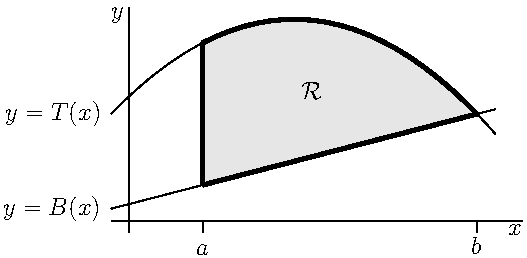
\includegraphics{vSliceA.pdf}
\end{center}
\end{efig}
We'll shortly express that mass 
as a two dimensional integral. As a warmup, recall the procedure that
we used  to set up a (one dimensional) integral representing the area 
of $\cR$ in Example \eref{CLP101}{eg areabetween riemann} of the CLP-2 text.
\begin{itemize}
\item 
Pick a natural number $n$ (that we will later send to infinity), and then 
\item 
subdivide $\cR$ into $n$ narrow vertical slices, each of width 
$\De x=\frac{b-a}{n}$. Denote by $x_i = a + i\,\De x$ the $x$-coordinate 
of the right hand edge of slice number $i$.
\begin{efig}
\begin{center}
   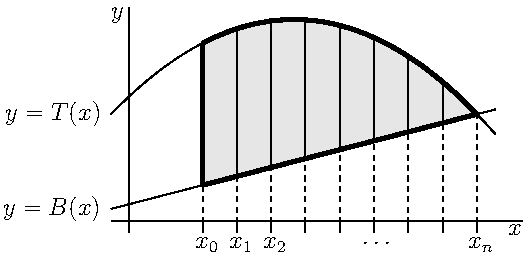
\includegraphics{vSliceB.pdf}
\end{center}
\end{efig}
\item 
For each $i=1,2,\dots,n$, slice number $i$ has $x$ running from $x_{i-1}$ 
to $x_i$. We approximate its area by the area of a rectangle. 
We pick a number $x_i^*$ between $x_{i-1}$ and $x_i$ and approximate the 
slice by a rectangle whose top is at $y=T(x_i^*)$ 
and whose bottom is at $y=B(x_i^*)$. The rectangle is outlined in blue in the 
figure below.
\begin{efig}
\begin{center}
   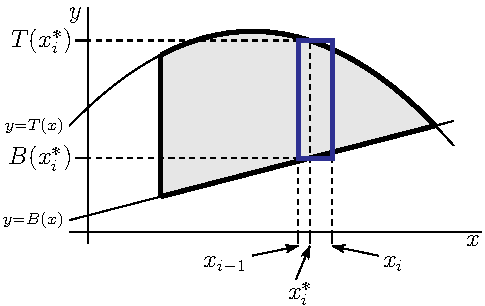
\includegraphics{vSliceC.pdf}
\end{center}
\end{efig}
\item 
Thus the area of slice $i$ is approximately $\big[T(x_i^*)-B(x_i^*)\big]\De x$.
\item 
So the Riemann sum approximation of the area of $\cR$ is
\begin{align*}
  \text{Area} &\approx \sum_{i=1}^n  \big[T(x_i^*)-B(x_i^*)\big]\De x
\end{align*}
\item 
By taking the limit as $n \to \infty$ (i.e. taking the limit as the width of the rectangles goes to zero), we convert the Riemann sum into a definite integral (see 
Definition~\eref{CLP101}{def:INTintegral} in the CLP-2 text) and at the 
same time our approximation of the area becomes the exact area:
\begin{align*}
\text{Area}
=\lim_{n\rightarrow\infty}\sum_{i=1}^n  \big[T(x_i^*)-B(x_i^*)\big]\De x
=\int_a^b \big[T(x)-B(x)\big]\dee{x} 
\end{align*}
\end{itemize}
Now we can expand that procedure to yield the mass of $\cR$ rather
than the area of $\cR$. We just have to replace our approximation
$\big[T(x_i^*)-B(x_i^*)\big]\De x$ of the area of slice $i$ by an
approximation to the mass of slice $i$. To do so, we
\begin{itemize}
\item 
Pick a natural number $m$ (that we will later send to infinity), and then 
\item 
subdivide slice number $i$ into $m$ tiny rectangles, each of width $\De x$ 
and of height $\De y=\frac{1}{m}\big[T(x_i^*)-B(x_i^*)\big]$. Denote by 
$y_j = B(x_i^*) + j\,\De y$ the $y$-coordinate 
of the top of rectangle number $j$.
\begin{efig}
\begin{center}
   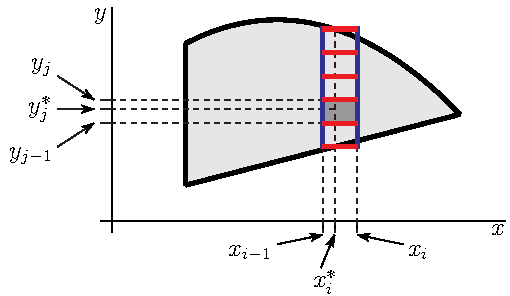
\includegraphics{vSliceD.pdf}
\end{center}
\end{efig}
\item 
At this point we approximate the density inside each rectangle by a constant.
For each $j=1,2,\dots,m$, rectangle number $j$ has $y$ running from $y_{j-1}$ 
to $y_j$.  We pick a number $y_j^*$ between $y_{j-1}$ and $y_j$ and 
approximate the density on rectangle number $j$ in slice number $i$
by the constant $f\big(x_i^*,y_j^*\big)$.
\item 
Thus the mass of rectangle number $j$ in slice number $i$ is approximately $f\big(x_i^*,y_j^*\big)\,\De x\,\De y$.
\item 
So the Riemann sum approximation of the mass of slice number $i$ is
\begin{align*}
  \text{Mass of slice $i$} 
          &\approx \sum_{j=1}^m  f\big(x_i^*,y_j^*\big)\,\De x\,\De y
\end{align*}
Note that the $y_j^*$'s depend on $i$ and $m$.
\item 
By taking the limit as $m \to \infty$ (i.e. taking the limit as the height 
of the rectangles goes to zero), we convert the Riemann sum into a definite integral:
\begin{align*}
  \text{Mass of slice $i$} 
          &\approx \De x \int_{B(x_i^*)}^{T(x_i^*)} f\big(x_i^*,y\big)\,\dee{y}
          = F(x_i^*)\,\De x
\end{align*}
where
\begin{equation*}
F(x) = \int_{B(x)}^{T(x)} f\big(x,y\big)\,\dee{y}
\end{equation*}
Notice that, while we started with the density $f(x,y)$ being a function of 
both $x$ and $y$, by taking the limit of this Riemann sum,
we have ``integrated out'' the dependence on $y$. 
As a result, $F(x)$ is a function of $x$ only, not of $x$ and $y$.

\item
Finally taking the limit as $n \to \infty$ (i.e. taking the limit as the slice 
width goes to zero), we get
\begin{align*}
\text{Mass}
&=\lim_{n\rightarrow\infty}\sum_{i=1}^n  
\De x \int_{B(x_i^*)}^{T(x_i^*)} f\big(x_i^*,y\big)\,\dee{y}
= \lim_{n\rightarrow\infty}\sum_{i=1}^n  F(x_i^*)\,\De x  
\end{align*}
Now we are back in familiar 1-variable territory. The sum 
$\sum\limits_{i=1}^n  F(x_i^*)\,\De x$ is a Riemann sum approximation
to the integral $ \int_a^b F(x)\,\dee{x}$. So
\begin{align*}
\text{Mass}
&= \int_a^b F(x)\,\dee{x}
=\int_a^b \left[\int_{B(x)}^{T(x)} f\big(x,y\big)\,\dee{y}\right]\dee{x} 
\end{align*}
\end{itemize}
This is our first double integral. There are a couple of different standard
notations for this integral.
\begin{notn}\label{notn dbl int}
\begin{align*}
\dblInt_\cR f\big(x,y\big)\,\dee{x}\,\dee{y}
&= \int_a^b \left[\int_{B(x)}^{T(x)} f\big(x,y\big)\,\dee{y}\right]\dee{x} \\
&=\int_a^b \int_{B(x)}^{T(x)} f\big(x,y\big)\,\dee{y}\,\dee{x}
=\int_a^b \dee{x} \int_{B(x)}^{T(x)} \dee{y}\, f\big(x,y\big)
\end{align*}
The last three integrals here are called iterated integrals, 
for obvious reasons.
\end{notn}
Note that
\begin{itemize}
\item 
to evaluate the integral 
$\displaystyle\int_a^b \int_{B(x)}^{T(x)} f\big(x,y\big)\,\dee{y}\,\dee{x}$,
\begin{itemize}
  \item
  first evaluate the inside integral 
  $\int_{B(x)}^{T(x)} f\big(x,y\big)\,\dee{y}$ using the inside
  limits of integration, and by treating $x$ as a constant and using 
  standard single variable integration techniques, such as those in the
  CLP-2 text. The result of the 
  inside integral is a function of $x$ only.  Call it $F(x)$.
  \item
   Then evaluate the outside integral $\int_a^b F(x)\,\dee{x}$,
   whose integrand is the answer to the inside integral. Again, this
   integral is evaluated using standard single variable integration 
   techniques.
\end{itemize}

\item
To evaluate the integral 
$\displaystyle\int_a^b \dee{x} \int_{B(x)}^{T(x)} \dee{y}\, f\big(x,y\big)$,
\begin{itemize}
  \item
  first evaluate the inside integral 
  $\int_{B(x)}^{T(x)} \dee{y}\, f\big(x,y\big)$ using the limits of 
  integration that are directly beside the $\dee{y}$. Indeed the $\dee{y}$
  is written directly beside $\int_{B(x)}^{T(x)}$ to make it clear that
  the limits of integration $B(x)$ and $T(x)$ are for the $y$-integral.
  In the past you probably wrote this integral as 
  $\int_{B(x)}^{T(x)} f\big(x,y\big)\ \dee{y}$. The result of 
  the inside integral is again a function of $x$ only.  Call it $F(x)$.
  \item
   Then evaluate the outside integral $\int_a^b \dee{x}\,F(x)$,
   whose integrand is the answer to the inside integral and whose limits
   of integration are directly beside the $\dee{x}$.
\end{itemize}
\end{itemize}

At this point you may be wondering ``Do we always have to use vertical 
slices?'' and ``Do we always have to integrate with respect to $y$ first?''
The answer is ``no''. This brings us to consider ``horizontal slices''.

\subsection{Horizontal Slices}
We found, when computing areas of regions in the $xy$-plane, that
it is often advantageous to use horizontal slices, rather than vertical
slices. See, for example,
Example \eref{CLP101}{eg:AREAb} in the CLP-2 text.
The same is true when setting up multidimensional integrals. So we now repeat
the setup procedure of the last section, but starting with horizontal slices, 
rather than vertical slices. This procedure will be useful when 
dealing with regions of the form
\begin{equation*}
\cR = \big\{\ (x,y)\ \big|\ c\le y\le d,\ L(y)\le x\le R(y)\ \big\}
\end{equation*}
\begin{efig}
\begin{center}
   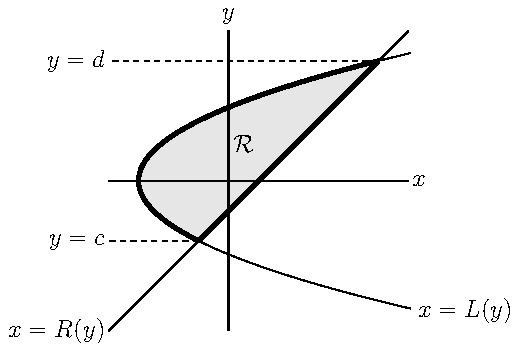
\includegraphics{hSliceA.pdf}
\end{center}
\end{efig}
Here $L(y)$ (``$L$'' stands for ``left'') is the smallest\footnote{
By the ``smallest '' $x$ we mean the $x$ farthest to the left along 
the number line, not the $x$ closest to $0$.} allowed 
value of $x$, when the $y$-coordinate is $y$, and 
$R(y)$ (``$R$'' stands for ``right'') is the largest allowed value 
of $x$, when the $y$-coordinate is $y$.
Suppose that we wish to evaluate the mass of a plate that
fills the region $\cR$, and that the density of the plate is $f(x,y)$. 
We follow essentially the same the procedure as we used 
with vertical slices, but with the roles of $x$ and $y$ swapped.
\begin{itemize}
 \item 
Pick a natural number $n$ (that we will later send to infinity). Then
 \item 
subdivide the interval $c\le y\le d$ into $n$ narrow subintervals, each 
of width $\De y=\frac{d-c}{n}$. Each subinterval cuts a thin horizontal 
slice from the region (see the figure below).
 \item We approximate slice number $i$ by a thin horizontal rectangle (indicated by the long darker gray rectangle in the figure below). On this 
slice, the $y$-coordinate runs over a very narrow range. 
We pick a number $y_i^*$, somewhere in that range. We approximate slice 
$i$ by a rectangle whose left side is at $x=L(y_i^*)$ and whose right side 
is at $x=R(y_i^*)$.
\item 
If we were computing the area of $\cR$, we would now
approximate the area of slice $i$ by $\big[R(x_i^*)-L(x_i^*)\big]\De y$,
which is the area of the rectangle with width $\big[R(x_i^*)-L(x_i^*)\big]$
and height $\De y$.
\item
To get the mass, just as we did above with vertical slices, we
\begin{itemize}
\item 
   pick another natural number $m$ (that we will later send to infinity), 
   and then 
\item 
   subdivide slice number $i$ into $m$ tiny rectangles, each of height $\De y$ 
and of width $\De x=\frac{1}{m}\big[R(y_i^*)-L(y_i^*)\big]$. 
%Denote by $x_j = L(y_i^*) + j\,\De x$ the $x$-coordinate 
%of the right hand edge of rectangle number $j$.
\item 
For each $j=1,2,\dots,m$, rectangle number $j$ has $x$ running over a very narrow range.  We pick a number $x_j^*$ somewhere in that range. 
See the small black rectangle in the figure below.
\begin{efig}
\begin{center}
   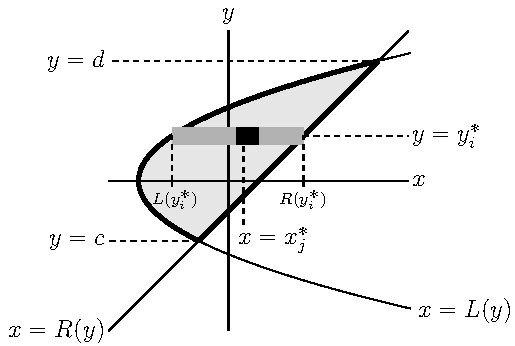
\includegraphics{hSliceB.pdf}
\end{center}
\end{efig}
Here is a magnified sketch of slice number $i$
\begin{efig}
\begin{center}
   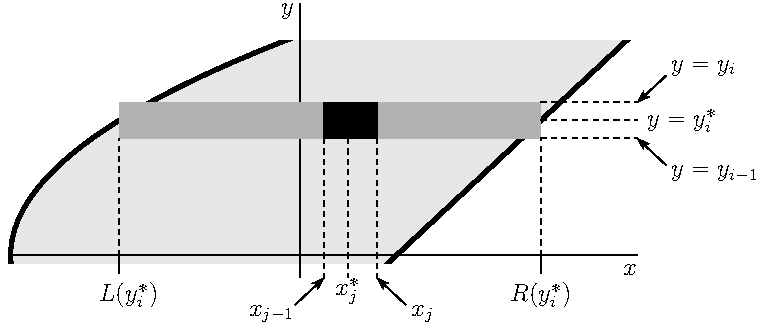
\includegraphics{hSliceBB.pdf}
\end{center}
\end{efig}

\item 
On rectangle number $j$ in slice number $i$, we approximate the density
by $f\big(x_j^*,y_i^*\big)$, giving us that
the mass of rectangle number $j$ in slice number $i$ is approximately $f\big(x_j^*,y_i^*\big)\,\De x\,\De y$.
\item 
So the Riemann sum approximation of the mass of (horizontal) slice number 
$i$ is
\begin{align*}
  \text{Mass of slice $i$} 
          &\approx \sum_{j=1}^m  f\big(x_j^*,y_i^*\big)\,\De x\,\De y
\end{align*}
\item 
By taking the limit as $m \to \infty$ (i.e. taking the limit as the width 
of the rectangles goes to zero), we convert the Riemann sum into a definite integral:
\begin{align*}
  \text{Mass of slice $i$} 
          &\approx \De y \int_{L(y_i^*)}^{R(y_i^*)} f\big(x,y_i^*\big)\,\dee{x}
          = F(y_i^*)\,\De y
\end{align*}
where
\begin{equation*}
F(y) = \int_{L(y)}^{R(y)} f\big(x,y\big)\,\dee{x}
\end{equation*}
Observe that, as $x$ has been integrated out, $F(y)$ is a function of $y$ 
only, not of $x$ and $y$.
\end{itemize}
\item
Finally taking the limit as $n \to \infty$ (i.e. taking the limit as the slice 
width goes to zero), we get
\begin{align*}
\text{Mass}
&=\lim_{n\rightarrow\infty}\sum_{i=1}^n  
\De y \int_{L(y_i^*)}^{R(y_i^*)} f\big(x,y_i^*\big)\,\dee{x}
= \lim_{n\rightarrow\infty}\sum_{i=1}^n  F(y_i^*)\,\De y  
\end{align*}
Now $\sum\limits_{i=1}^n  F(y_i^*)\,\De y$ is a Riemann sum approximation
to the integral $ \int_c^d F(y)\,\dee{y}$. So
\begin{align*}
\text{Mass}
&= \int_c^d F(y)\,\dee{y}
=\int_c^d \left[\int_{L(y)}^{R(y)} f\big(x,y\big)\,\dee{x}\right]\dee{y} 
\end{align*}
\end{itemize}
The standard notations of Notation \ref{notn dbl int} also
apply to this integral.
\begin{notn}\label{notn dbl int again}
\begin{align*}
\dblInt_\cR f\big(x,y\big)\,\dee{x}\,\dee{y}
&=\int_c^d \left[\int_{L(y)}^{R(y)} f\big(x,y\big)\,\dee{x}\right]\dee{y} \\
&=\int_c^d \int_{L(y)}^{R(y)} f\big(x,y\big)\,\dee{x}\,\dee{y}
=\int_c^d \dee{y} \int_{L(y)}^{R(y)} \dee{x}\, f\big(x,y\big)
\end{align*}
\end{notn}
Note that
\begin{itemize}
\item 
to evaluate the integral 
$\displaystyle\int_c^d \int_{L(y)}^{R(y)} f\big(x,y\big)\,\dee{x}\,\dee{y}$,
\begin{itemize}
  \item
  first evaluate the inside integral 
  $\int_{L(y)}^{R(y)} f\big(x,y\big)\,\dee{x}$ using the inside
  limits of integration. The result of the inside integral is a function
  of $y$ only.  Call it $F(y)$.
  \item
   Then evaluate the outside integral $\int_c^d F(y)\,\dee{y}$,
   whose integrand is the answer to the inside integral.
\end{itemize}

\item
To evaluate the integral 
$\displaystyle\int_c^d \dee{y} \int_{L(y)}^{R(y)} \dee{x}\, f\big(x,y\big)$,
\begin{itemize}
  \item
  first evaluate the inside integral 
  $\int_{L(y)}^{R(y)} \dee{x}\, f\big(x,y\big)$ using the limits of 
  integration that are directly beside the $\dee{x}$. 
  Again, the $\dee{x}$
  is written directly beside $\int_{L(y)}^{R(y)}$ to make it clear that
  the limits of integration $L(y)$ and $R(y)$ are for the $x$-integral.
  In the past you probably wrote this integral as 
  $\int_{L(y)}^{R(y)} f\big(x,y\big)\ \dee{x}$.
  The result of the inside integral is again a function of $y$ only.  
  Call it $F(y)$.
  \item
   Then evaluate the outside integral $\int_c^d \dee{y}\,F(y)$,
   whose integrand is the answer to the inside integral and whose limits
   of integration are directly beside the $\dee{y}$.
\end{itemize}
\end{itemize}

By way of summary, we now have two integral representations
for the mass of regions in the $xy$-plane.
\begin{theorem}\label{thm xy mass}
Let $\cR$ be a region in the $xy$-plane and let the function 
$f(x,y)$ be defined and continuous on $\cR$.
\begin{enumerate}[(a)]
\item If
\begin{align*}
\cR=\big\{\ (x,y)\ \big|\ a\le x\le b,\ B(x)\le y\le T(x)\ \big\}
\end{align*}
with $B(x)$ and $T(x)$ being continuous, and if the mass density in $\cR$ 
is $f(x,y)$, then the mass of $\cR$
is
\begin{equation*}
\int_a^b \left[\int_{B(x)}^{T(x)} f\big(x,y\big)\,\dee{y}\right]\dee{x}
=\int_a^b \int_{B(x)}^{T(x)} f\big(x,y\big)\,\dee{y}\,\dee{x}
=\int_a^b \dee{x} \int_{B(x)}^{T(x)} \dee{y}\, f\big(x,y\big)
\end{equation*}

\item If
\begin{equation*}
\cR = \big\{\ (x,y)\ \big|\ c\le y\le d,\ L(y)\le x\le R(y)\ \big\}
\end{equation*}
with $L(y)$ and $R(y)$ being continuous, 
and if the mass density in $\cR$ is $f(x,y)$, then the mass of $\cR$
is
\begin{equation*}
\int_c^d \left[\int_{L(y)}^{R(y)} f\big(x,y\big)\,\dee{x}\right]\dee{y}
=\int_c^d \int_{L(y)}^{R(y)} f\big(x,y\big)\,\dee{x}\,\dee{y}
=\int_c^d \dee{y} \int_{L(y)}^{R(y)} \dee{x}\, f\big(x,y\big)
\end{equation*}
\end{enumerate}
\end{theorem}
\noindent
Implicit in Theorem  \ref{thm xy mass} is the statement that, if
\begin{align*}
&\big\{\ (x,y)\ \big|\ a\le x\le b,\ B(x)\le y\le T(x)\ \big\} \\
   =& \big\{\ (x,y)\ \big|\ c\le y\le d,\ L(y)\le x\le R(y)\ \big\}
\end{align*}
and if $f(x,y)$ is continuous, then
\begin{equation*}
\int_a^b \int_{B(x)}^{T(x)} f\big(x,y\big)\,\dee{y}\,\dee{x}
=\int_c^d \int_{L(y)}^{R(y)} f\big(x,y\big)\,\dee{x}\,\dee{y}
\end{equation*}
This is called Fubini's theorem\footnote{This theorem is named after the Italian mathematician Guido Fubini (1879--1943).
% He proved that a double integral can be evaluated as an iterated integral
% when the integrand is absolutely integrable.
% Euler proved the special case of a continuous integrand on a product of
% closed bouded subsets in the 18th century.
}. It will be discussed more in the
optional \S\ref{sec def int more}. 

\begin{notn}\label{notn double integral yet again}
The integrals of Theorem \ref{thm xy mass} are often denoted 
\begin{equation*}
\dblInt_\cR f(x,y)\,\dee{x}\dee{y} \qquad\text{or}\qquad
\dblInt_\cR f(x,y)\,\dee{A} 
\end{equation*}
The symbol $\dee{A}$ represents the area of an ``infinitesimal'' piece
of $\cR$.
\end{notn}

Here is a simple example. We'll do some more complicated examples in
\S\ref{sec int examples}.

\begin{eg}\label{eg dblInt 0}
Let $\cR$ be the triangular region above the $x$-axis, to the right of
the $y$-axis and to the left of the line $x+y=1$. 
Find the mass of $\cR$ if it has density $f(x,y)=y$.

\soln We'll do this problem twice --- once using vertical strips and
once using horizontal strips. First, here is a sketch of $\cR$.
\begin{efig}
\begin{center}
   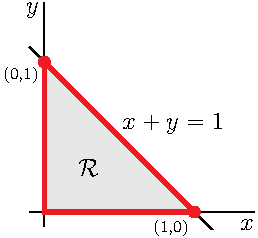
\includegraphics{dblInt0a.pdf}
\end{center}
\end{efig}


\medskip\noindent\emph{Solution using vertical strips.}\ \ \
We'll now set up a double integral for the mass using vertical strips.  
Note, from the figure 
\begin{efig}
\begin{center}
   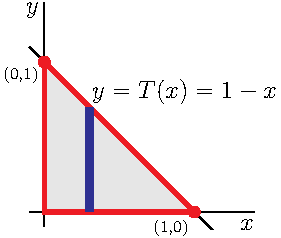
\includegraphics{dblInt0b.pdf}
\end{center}
\end{efig}
that
\begin{itemize}
\item
the leftmost points in $\cR$ have $x=0$ and the rightmost point
in $\cR$ has $x=1$ and
\item 
for each fixed $x$ between $0$ and $1$, the point $(x,y)$ in $\cR$
with the smallest $y$ has $y=0$ and the point $(x,y)$ in $\cR$
with the largest $y$ has $y=1-x$.
\end{itemize}
Thus
\begin{equation*}
\cR=\Set{(x,y)}{0=a\le x\le b=1,\ 
        0= B(x)\le y\le T(x) = 1-x}
\end{equation*}
and, by part (a) of Theorem  \ref{thm xy mass}
\begin{align*}
\text{Mass} &= \int_a^b \dee{x} \int_{B(x)}^{T(x)} \dee{y}\, f\big(x,y\big) 
        = \int_0^1 \dee{x} \int_0^{1-x} \dee{y}\, y 
\end{align*}
Now the inside integral is
\begin{align*}
\int_0^{1-x}  y \ \dee{y}
=\left[ \frac{y^2}{2} \right]_0^{1-x}
=\frac{1}{2}(1-x)^2
\end{align*}
so that the
\begin{align*}
\text{Mass} &= \int_0^1 \dee{x}\  \frac{(1-x)^2}{2}
        =\left[-\frac{(1-x)^3}{6}\right]_0^1 
        = \frac{1}{6}
\end{align*} 


\medskip\noindent\emph{Solution using horizontal strips.}\ \ \
This time we'll set up a double integral for the mass using horizontal strips.  
Note, from the figure 
\begin{efig}
\begin{center}
   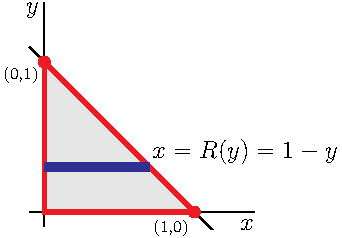
\includegraphics{dblInt0c.pdf}
\end{center}
\end{efig}
that
\begin{itemize}
\item
the lowest points in $\cR$ have $y=0$ and the topmost point
in $\cR$ has $y=1$ and
\item 
for each fixed $y$ between $0$ and $1$, the point $(x,y)$ in $\cR$
with the smallest $x$ has $x=0$ and the point $(x,y)$ in $\cR$
with the largest $x$ has $x=1-y$.
\end{itemize}
Thus
\begin{equation*}
\cR=\Set{(x,y)}{0=c\le y\le d=1,\ 
        0= L(y)\le x\le R(y) = 1-y}
\end{equation*}
and, by part (b) of Theorem  \ref{thm xy mass}
\begin{align*}
\text{Mass} &= \int_c^d \dee{y} \int_{L(y)}^{R(y)} \dee{x}\, f\big(x,y\big) 
        = \int_0^1 \dee{y} \int_0^{1-y} \dee{x}\, y 
\end{align*}
Now the inside integral is
\begin{align*}
\int_0^{1-y}  y \ \dee{x}
=\left[ xy \right]_0^{1-y}
=y-y^2
\end{align*}
since the $y$ integral treats $x$ as a constant.
So the
\begin{align*}
\text{Mass} &= \int_0^1 \dee{y}\  \big[y-y^2\big]
        =\left[\frac{y^2}{2}-\frac{y^3}{3}\right]_0^1 
        = \frac{1}{2}-\frac{1}{3}
        =\frac{1}{6}
\end{align*} 
\end{eg}


Double integrals share the usual basic properties that we are used to from 
integrals of functions of one variable. See, for example,
Theorem \eref{CLP101}{thm:Intarith} and Theorem \eref{CLP101}{thm:INTineq} 
in the CLP-2 text. Indeed the following theorems follow from them.
\begin{theorem}[Arithmetic of Integration]\label{thm:Int2darith}
Let $A,B,C$ be real numbers. Under the hypotheses of 
Theorem \ref{thm xy mass},
\begin{align*}
\text{(a)}&& \dblInt_\cR \left( f(x,y) + g(x,y) \right)\,\dee{x}\dee{y}
&= \dblInt_\cR f(x,y)\,\dee{x}\dee{y} + \dblInt_\cR g(x,y)\,\dee{x}\dee{y}\\
%
\text{(b)}&&
\dblInt_\cR\left(f(x,y)-g(x,y)\right)\,\dee{x}\dee{y} 
&= \dblInt_\cR f(x,y)\,\dee{x}\dee{y} - \dblInt_\cR g(x,y)\,\dee{x}\dee{y}\\
%
\text{(c)}&& \dblInt_\cR C f(x,y)\,\dee{x}\dee{y}
&= C\,\dblInt_\cR f(x,y)\,\dee{x}\dee{y} 
\end{align*}
\end{theorem}

\addtocounter{theorem}{-1}
\begin{theorem}[continued]
Combining these three rules we have
\begin{align*}
\text{(d)}&& \dblInt_\cR\left( Af(x,y) + Bg(x,y) \right)\,\dee{x}\dee{y}
&= A\dblInt_\cR f(x,y)\,\dee{x}\dee{y} 
            + B\dblInt_\cR g(x,y)\,\dee{x}\dee{y}
\intertext{That is, integrals depend linearly on the integrand.}
%
\text{(e)}&& \dblInt_\cR \,\dee{x}\dee{y} &= \text{Area}(\cR) \\
%
\intertext{If the region $\cR$ in the $xy$-plane is the union of regions $\cR_1$ and $\cR_2$ that do not overlap (except possibly on their boundaries),
then}
\text{(f)}&& \dblInt_\cR f(x,y)\,\dee{x}\dee{y} 
                  &= \dblInt_{\cR_1} f(x,y)\,\dee{x}\dee{y}
                    +\dblInt_{\cR_2} f(x,y)\,\dee{x}\dee{y} 
\end{align*}
\begin{center}
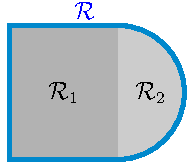
\includegraphics{union}\qquad\qquad\qquad\includegraphics{unionB}
\end{center}
\end{theorem}

In the very special (but not that uncommon) case that $\cR$ is the 
rectangle 
\begin{equation*}
\cR=\Set{(x,y)}{a\le x\le b,\ c\le y\le d}
\end{equation*} 
and the integrand is the product $f(x,y)=g(x)h(y)$,
\begin{align*}
\dblInt_\cR f(x,y)\,\dee{x}\dee{y}
&=\int_a^b\dee{x} \int_c^d\dee{y}\ g(x) h(y) \\
&=\int_a^b\dee{x}\ g(x) \int_c^d\dee{y}\  h(y) \\
&\hskip0.5in\text{since $g(x)$ is a constant as far as the $y$-integral is concerned} \\
&=\left[ \int_a^b\dee{x}\ g(x)\right]\ \left[\int_c^d\dee{y}\  h(y)\right] \\
&\hskip0.5in\text{since $\int_c^d\dee{y}\  h(y)$ is a constant as far 
as the $x$-integral is concerned}
\end{align*}
This is worth stating as a theorem

\begin{theorem}\label{thm factorize}
If the domain of integration
\begin{equation*}
\cR=\Set{(x,y)}{a\le x\le b,\ c\le y\le d}
\end{equation*} 
is a rectangle and the integrand is the product $f(x,y)=g(x)h(y)$, then
\begin{equation*}
\dblInt_\cR f(x,y)\,\dee{x}\dee{y}
=\left[ \int_a^b\dee{x}\ g(x)\right]\ \left[\int_c^d\dee{y}\  h(y)\right] 
\end{equation*}
\end{theorem}

Just as was the case for single variable integrals, sometimes we don't
actually need to know the value of a double integral exactly. We are
instead interested in bounds on its value. 
The following theorem provides some simple tools for generating such bounds.
They are the multivariable analogs of the single variable tools in
Theorem \eref{CLP101}{thm:INTineq} of the CLP-2 text.  


\begin{theorem}[Inequalities for Integrals]\label{thm:INT2dineq}
Under the hypotheses of Theorem \ref{thm xy mass},
\begin{enumerate}[(a)]
\item 
If $f(x,y)\ge 0$ for all $(x,y)$ in $\cR$, then
\begin{align*}
\dblInt_\cR f(x,y)\,\dee{x}\dee{y} \ge 0
\end{align*}
\item 
If there are constants $m$ and $M$ such that  $m\le f(x,y)\le M$ 
for all $(x,y)$ in $\cR$, then
\begin{align*}
m\,\text{Area}(\cR)\le \dblInt_\cR f(x,y)\,\dee{x}\dee{y} 
                                   \le M\,\text{Area}(\cR)
\end{align*}
\item If $f(x,y)\le g(x,y)$ for all $(x,y)$ in $\cR$, then
\begin{align*}
\dblInt_\cR f(x,y)\,\dee{x}\dee{y} \le \dblInt_\cR g(x,y)\,\dee{x}\dee{y}
\end{align*}
\item We have
\begin{align*}
\left|\dblInt_\cR f(x,y)\,\dee{x}\dee{y}\right|
          \le \dblInt_\cR |f(x,y)|\,\dee{x}\dee{y}
\end{align*}
\end{enumerate}
\end{theorem}




\subsection{Volumes}

Now that we have defined double integrals, we should start putting them to use.
One of the most immediate applications arises from interpreting $f(x,y)$,
not as a density, but rather as the height of the part of a solid above the 
point $(x,y)$ in the $xy$-plane. Then Theorem \ref{thm xy mass} gives 
the volume between the $xy$-plane and the surface $z=f(x,y)$. 

We'll now see how this goes in the case of part (b)
of Theorem \ref{thm xy mass}. The case of part (a) works in the same way.
So we assume that the solid $\cV$ lies above the base region
\begin{equation*}
\cR = \big\{\ (x,y)\ \big|\ c\le y\le d,\ L(y)\le x\le R(y)\ \big\}
\end{equation*}
and that
\begin{equation*}
\cV = \big\{\ (x,y,z)\ \big|\ (x,y)\in\cR,\  0\le z\le f(x,y)\ \big\}
\end{equation*}
The base region $\cR$ (which is also the top view of $\cV$)
is sketched in the figure on the left below and
the part of $\cV$ in the first octant is sketched in the figure on the right below.
\begin{efig}
\begin{center}
   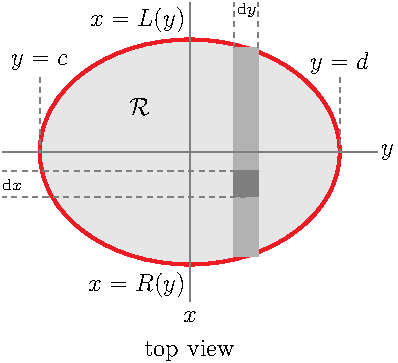
\includegraphics{volSliceB.pdf}\qquad
   \raisebox{0.2\height}{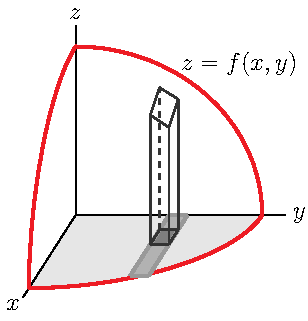
\includegraphics{volSliceA.pdf}}
\end{center}
\end{efig}
To find the volume of $\cV$ we shall
\begin{itemize}
\item
Pick a natural number $n$ and slice $\cR$ into strips of width
$\De y=\frac{d-c}{n}$.
\item
  Subdivide slice number $i$ into $m$ tiny rectangles, each of height $\De y$ 
and of width $\De x=\frac{1}{m}\cdots$. 
\item 
  Compute, approximately, the volume of the part of $\cV$ that is above 
  each rectangle.
\item
 Take the limit $m\rightarrow\infty$ and then the limit $n\rightarrow\infty$.
\end{itemize}
We have just been through this type of argument twice. So we'll
abbreviate the argument and just say
\begin{itemize}
\item
   slice the base region $\cR$ into long ``infinitesimally'' thin strips of width $\dee{y}$.
\item
   Subdivide each strip into ``infinitesimal'' rectangles each of 
height $\dee{y}$ and of width $\dee{x}$. See the figure on the left above.
\item
  The volume of the part of $\cV$ that is above the rectangle centred on $(x,y)$
        is essentially $f(x,y)\,\dee{x}\,\dee{y}$. See the figure on 
        the right above.
\item 
   So the volume of the part of $\cV$ that is above the strip centred on $y$
        is essentially\footnote{Think of the part of $\cV$ that is above the                 strip as being a thin slice of bread. 
        Then the factor $\dee{y}$ in $\dee{y}\int_{L(y)}^{R(y)}\dee{x}\ f(x,y)$
is the thickness of the slice of bread. The factor
             $\int_{L(y)}^{R(y)}\dee{x}\ f(x,y)$ is the surface area
             of the constant $y$ cross-section 
             $\Set{(x,z)}{L(y)\le x\le R(y),\ 0\le z\le f(x,y)}$, i.e. 
             the surface area of the slice of bread. }
 $\dee{y}\int_{L(y)}^{R(y)}\dee{x}\ f(x,y)$ and  
\item
   we arrive at the following conclusion.
\end{itemize}

\begin{impeqn}\label{eqn Volume y slice}
If 
\begin{equation*}
\cV = \big\{\ (x,y,z)\ \big|\ (x,y)\in\cR,\  0\le z\le f(x,y)\ \big\}
\end{equation*}
where
\begin{equation*}
\cR = \big\{\ (x,y)\ \big|\ c\le y\le d,\ L(y)\le x\le R(y)\ \big\}
\end{equation*}
then
\begin{equation*}
    \text{Volume}(\cV)
        =\int_c^d \dee{y}\int_{L(y)}^{R(y)} \dee{x}\ f(x,y)
\end{equation*}
\end{impeqn}
Similarly
 \begin{impeqn}\label{eqn Volume x slice}
If 
\begin{equation*}
\cV = \big\{\ (x,y,z)\ \big|\ (x,y)\in\cR,\  0\le z\le f(x,y)\ \big\}
\end{equation*}
where
\begin{equation*}
\cR = \big\{\ (x,y)\ \big|\ a\le x\le b,\ B(x)\le y\le T(x)\ \big\}
\end{equation*}
then
\begin{equation*}
    \text{Volume}(\cV)
        =\int_a^b \dee{x}\int_{B(x)}^{T(x)} \dee{y}\ f(x,y)
\end{equation*}
\end{impeqn}


\goodbreak
\subsection{Examples}
\label{sec int examples}

Oof --- we have had lots of equations and theory. It's time to put
all of this to work. Let's start with a mass example and then move on to 
a volume example. You will notice that the mathematics is really very
similar. Just the interpretation changes. 


\begin{eg}[Mass]\label{eg dblInt A}
Let $\nu>0$ be a constant and let $\cR$ be the region above the curve 
$x^2=4\nu y$ and to the right of the curve $y^2=\frac{1}{2}\nu x$. 
Find the mass of $\cR$ if it has density $f(x,y)=xy$.

\soln For practice, we'll do this problem twice --- once using vertical 
strips and once using horizontal strips. We'll start by sketching $\cR$.
First note that, since $y\ge\frac{x^2}{4\nu}$ and $x\ge \frac{2y^2}{\nu}$, 
both $x$ and $y$ are positive throughout $\cR$.
The two curves intersect at points $(x,y)$ that satisfy both
\begin{align*}
x = \frac{2y^2}{\nu}\text{ and }y=\frac{x^2}{4\nu}
\quad\implies\quad x  = \frac{2y^2}{\nu} = \frac{2}{\nu}\left(\frac{x^2}{4\nu}\right)^2
                 = \frac{x^4}{8\nu^3}
\quad\iff\quad \left(\frac{x^3}{8\nu^3}-1\right)x=0
\end{align*}
This equation has only two real\footnote{It also has two complex solutions that
play no role here.} solutions --- $x=0$ and $x=2\nu$.
So the upward opening parabola $y = \frac{x^2}{4\nu}$ and the 
rightward opening parabola $x=\frac{2y^2}{\nu}$  intersect at $(0,0)$ and $(2\nu,\nu)$.
\begin{efig}
\begin{center}
   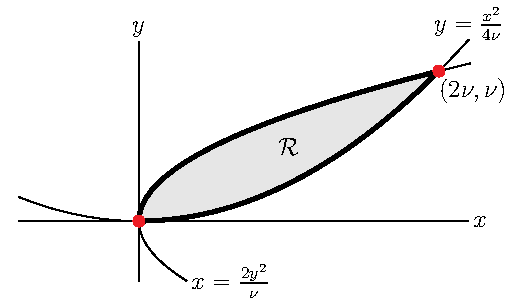
\includegraphics{dblIntAa.pdf}
\end{center}
\end{efig}


\medskip\noindent\emph{Solution using vertical strips.}\ \ \
We'll now set up a double integral for the mass using vertical strips
and using the abbreviated argument of the end of the last section 
(on volumes).  Note, from the figure above, that
\begin{equation*}
\cR=\bigg\{(x,y)\ \bigg|\ 0=a\le x\le b=2\nu,\ 
        \frac{x^2}{4\nu}= B(x)\le y\le T(x) = \sqrt{\frac{\nu x}{2}}\ \bigg\}
\end{equation*}
\begin{itemize}
\item
   Slice $\cR$ into long ``infinitesimally'' thin 
   vertical strips of width $\dee{x}$.
\item
   Subdivide each strip into ``infinitesimal'' rectangles each of 
   height $\dee{y}$ and of width $\dee{x}$. See the figure below.
\begin{efig}
\begin{center}
   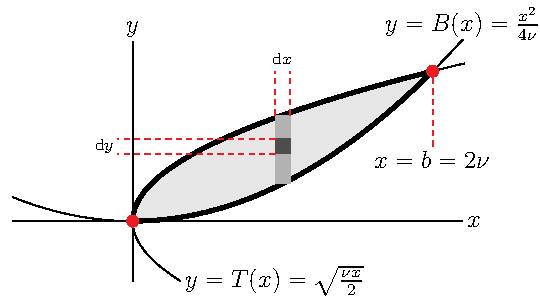
\includegraphics{dblIntAb.pdf}
\end{center}
\end{efig}

\item
  The mass of the rectangle centred on $(x,y)$
        is essentially $f(x,y)\,\dee{x}\,\dee{y}=xy\,\dee{x}\,\dee{y}$.
\item 
   So the mass of the strip centred on $x$ is 
         essentially $\ \dee{x}\, \int_{B(x)}^{T(x)}\dee{y}\ f(x,y) $ 
   (the integral over $y$ adds up the masses of all of the different rectangles     on the single vertical strip in question) and  
\item
   we conclude that the
\begin{align*}
    \text{Mass}(\cR)
        &=\int_a^b \dee{x}\int_{B(x)}^{T(x)} \dee{y}\ f(x,y) 
         =\int_0^{2\nu} \dee{x}\int_{x^2/(4\nu)}^{\sqrt{\nu x/2}} \dee{y}\ xy 
\end{align*}
Here the integral over $x$ adds up the masses of all of the different strips.

Recall that, when integrating $y$, $x$ is held constant, so we may factor the
constant $x$ out of the inner $y$ integral.
\begin{align*}
\int_{x^2/(4\nu)}^{\sqrt{\nu x/2}} \dee{y}\ xy
&= x\int_{x^2/(4\nu)}^{\sqrt{\nu x/2}} \dee{y}\ y \\
&= x\left[\frac{y^2}{2}\right]_{x^2/(4\nu)}^{\sqrt{\nu x/2}} \\
&=\frac{\nu x^2}{4}-\frac{x^5}{32\nu^2}
\end{align*}
and the 
\begin{align*}
\text{Mass}(\cR)
%        &=\int_0^{2\nu} \dee{x}\  x\left[
%                 \int_{x^2/(4\nu)}^{\sqrt{\nu x/2}} \dee{y}\ y\right] \\
%        &=\int_0^{2\nu} \dee{x}\  x\left[\frac{y^2}{2}\right]
%                                     _{x^2/(4\nu)}^{\sqrt{\nu x/2}} \\
        &=\int_0^{2\nu} \dee{x}\ 
             \left[\frac{\nu x^2}{4}-\frac{x^5}{32\nu^2}\right] \\
        &= \frac{\nu (2\nu)^3}{3\times 4}-\frac{(2\nu)^6}{6\times 32\nu^2}
         =\frac{\nu^4}{3}
\end{align*}
\end{itemize}


\medskip\noindent\emph{Solution using horizontal strips.}\ \ \
We'll now set up a double integral for the mass using horizontal strips,
again using the abbreviated argument of the end of the last section 
(on volumes).  Note, from the figure at the beginning of this example, that
\begin{equation*}
\cR=\bigg\{(x,y)\ \bigg|\ 0=c\le y\le d=\nu,\ 
       \frac{2 y^2}{\nu} = L(y)\le x\le R(y) = \sqrt{4\nu y} \ \bigg\}
\end{equation*}
\begin{itemize}
\item
   Slice $\cR$ into long ``infinitesimally'' thin 
   horizontal strips of width $\dee{y}$.
\item
   Subdivide each strip into ``infinitesimal'' rectangles each of 
   height $\dee{y}$ and of width $\dee{x}$. See the figure below.
\begin{efig}
\begin{center}
   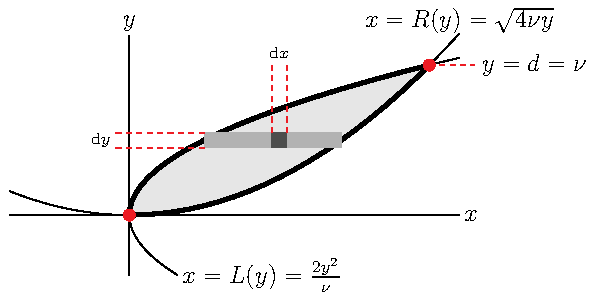
\includegraphics{dblIntAc.pdf}
\end{center}
\end{efig}

\item
  The mass of the rectangle centred on $(x,y)$
        is essentially $f(x,y)\,\dee{x}\,\dee{y}=xy\,\dee{x}\,\dee{y}$.
\item 
   So the mass of the strip centred on $y$ is 
         essentially $\ \dee{y}\, \int_{L(y)}^{R(y)}\dee{x}\ f(x,y) $ 
   (the integral over $x$ adds up the masses of all of the different rectangles     on the single horizontal strip in question) and  
\item
   we conclude that the
\begin{align*}
    \text{Mass}(\cR)
        &=\int_c^d \dee{y}\int_{L(y)}^{R(y)} \dee{x}\ f(x,y) 
         =\int_0^{\nu} \dee{y}\int_{2y^2/\nu}^{\sqrt{4\nu y}} \dee{x}\ xy 
\end{align*}
Here the integral over $y$ adds up the masses of all of the different strips.
Recalling that, when integrating $x$, $y$ is held constant
\begin{align*}
\text{Mass}(\cR)
        &=\int_0^{\nu} \dee{y}\  y\left[
                 \int_{2y^2/\nu}^{\sqrt{4\nu y}} \dee{x}\ x\right] \\
        &=\int_0^{\nu} \dee{y}\  y\left[\frac{x^2}{2}\right]
                                     _{2y^2/\nu}^{\sqrt{4\nu y}} \\
        &=\int_0^{\nu} \dee{y}\ 
             \left[2\nu y^2-\frac{2y^5}{\nu^2}\right] \\
        &= \frac{2\nu (\nu)^3}{3}-\frac{2\nu^6}{6\nu^2}
         =\frac{\nu^4}{3}
\end{align*}
\end{itemize}
\end{eg}

\begin{eg}[Volume]\label{eg dblInt V0}
Let $\cR$ be the part of the $xy$-plane above the $x$-axis and below 
the parabola $y=1-x^2$. Find the volume between $\cR$ and the surface
$z=x^2\sqrt{1-y}$.

\soln
Yet again, for practice, we'll do this problem twice --- once using 
vertical strips and once using horizontal strips. First, here is a 
sketch of $\cR$.
\begin{efig}
\begin{center}
   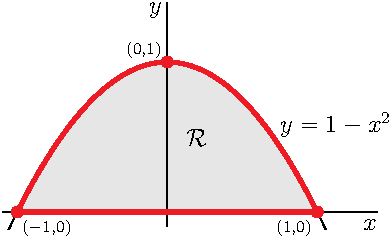
\includegraphics{dblIntV0a.pdf}
\end{center}
\end{efig}


\medskip\noindent\emph{Solution using vertical strips.}\ \ \
We'll now set up a double integral for the volume using vertical strips.  
Note, from the figure 
\begin{efig}
\begin{center}
   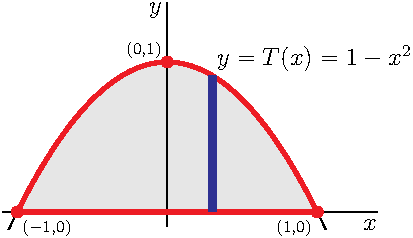
\includegraphics{dblIntV0b.pdf}
\end{center}
\end{efig}
that
\begin{itemize}
\item
the leftmost point in $\cR$ has $x=-1$ and the rightmost point
in $\cR$ has $x=1$ and
\item 
for each fixed $x$ between $-1$ and $1$, the point $(x,y)$ in $\cR$
with the smallest $y$ has $y=0$ and the point $(x,y)$ in $\cR$
with the largest $y$ has $y=1-x^2$.
\end{itemize}
Thus
\begin{equation*}
\cR=\Set{(x,y)}{-1=a\le x\le b=1,\ 
        0= B(x)\le y\le T(x) = 1-x^2}
\end{equation*}
and, by \eqref{eqn Volume x slice}
\begin{align*}
\text{Volume} &= \int_a^b \dee{x} \int_{B(x)}^{T(x)} \dee{y}\, f\big(x,y\big) 
        = \int_{-1}^1 \dee{x} \int_0^{1-x^2} \dee{y}\  x^2\sqrt{1-y}  \\
&=2\int_0^1 \dee{x} \int_0^{1-x^2} \dee{y}\  x^2\sqrt{1-y}
\end{align*}
since the inside integral $F(x) =  \int_0^{1-x^2} \dee{y}\  x^2\sqrt{1-y}$
is an even function of $x$.
Now, for $x\ge 0$, the inside integral is
\begin{align*}
\int_0^{1-x^2}  x^2\sqrt{1-y} \ \dee{y}
= x^2 \int_0^{1-x^2}  \sqrt{1-y} \ \dee{y}
=x^2 \left[ -\frac{2}{3}(1-y)^{3/2} \right]_0^{1-x^2}
=\frac{2}{3}x^2\big(1-x^3\big) 
\end{align*}
so that the
\begin{align*}
\text{Volume} &= 2\int_0^1 \dee{x}\ \frac{2}{3}x^2\big(1-x^3\big)
=\frac{4}{3}\left[\frac{x^3}{3}-\frac{x^6}{6}\right]_0^1
=\frac{2}{9}
\end{align*} 


\medskip\noindent\emph{Solution using horizontal strips.}\ \ \
This time we'll set up a double integral for the volume using horizontal strips.  
Note, from the figure 
\begin{efig}
\begin{center}
   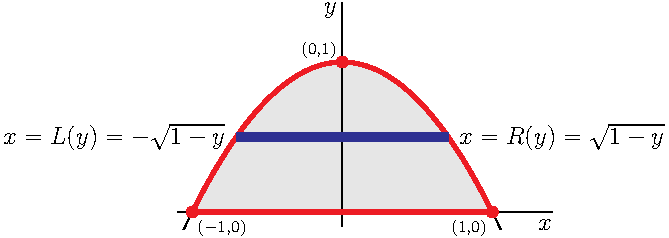
\includegraphics{dblIntV0c.pdf}
\end{center}
\end{efig}
that
\begin{itemize}
\item
the lowest points in $\cR$ have $y=0$ and the topmost point
in $\cR$ has $y=1$ and
\item 
for each fixed $y$ between $0$ and $1$, the point $(x,y)$ in $\cR$
with the leftmost $x$ has $x=-\sqrt{1-y}$ and the point $(x,y)$ in $\cR$
with the rightmost $x$ has $x=\sqrt{1-y}$.
\end{itemize}
Thus
\begin{equation*}
\cR=\Set{(x,y)}{0=c\le y\le d=1,\ 
        -\sqrt{1-y}= L(y)\le x\le R(y) = \sqrt{1-y}}
\end{equation*}
and, by \eqref{eqn Volume y slice}
\begin{align*}
\text{Volume} &= \int_c^d \dee{y} \int_{L(y)}^{R(y)} \dee{x}\, f\big(x,y\big) 
    = \int_0^1 \dee{y} \int_{-\sqrt{1-y}}^{\sqrt{1-y}} \dee{x}\, x^2\sqrt{1-y} 
\end{align*}
Now the inside integral has an even integrand (in $x$) and so is
\begin{align*}
\int_{-\sqrt{1-y}}^{\sqrt{1-y}} \dee{x}\, x^2\sqrt{1-y}
=2\sqrt{1-y}\int_0^{\sqrt{1-y}} x^2\ \dee{x}
=2\sqrt{1-y} \left[ \frac{x^3}{3} \right]_0^{\sqrt{1-y}}
=\frac{2}{3}(1-y)^2
\end{align*}
So the
\begin{align*}
\text{Volume} &= \frac{2}{3}\int_0^1 \dee{y}\  (1-y)^2
        =\frac{2}{3}\left[-\frac{(1-y)^3}{3}\right]_0^1 
        =\frac{2}{9}
\end{align*} 
\end{eg}


\begin{eg}[Volume]\label{eg dblInt B}
Find the volume common to the two cylinders $x^2+y^2=a^2$ and
$x^2+z^2=a^2$.

\soln
Our first job is figure out what the specified solid looks like. 
Note that
\begin{itemize}
\item
The variable $z$ does not appear in the equation $x^2+y^2=a^2$.
So, for every value of the constant $z_0$ the part of the cylinder
$x^2+y^2=a^2$ in the plane $z=z_0$, is the circle $x^2+y^2=a^2$, $z=z_0$.
So the cylinder $x^2+y^2=a^2$ consists of many circles stacked
vertically, one on top of the other. The part of the cylinder
$x^2+y^2=a^2$ that lies above the $xy$-plane is sketched in the
figure on the left below.

\item
The variable $y$ does not appear in the equation $x^2+z^2=a^2$.
So, for every value of the constant $y_0$ the part of the cylinder
$x^2+z^2=a^2$ in the plane $y=y_0$, is the circle $x^2+z^2=a^2$, $y=y_0$.
So the cylinder $x^2+z^2=a^2$ consists of many circles stacked
horizontally, one beside the other. The part of the cylinder
$x^2+z^2=a^2$ that lies to the right of the $xz$-plane is sketched in the
figure on the right below.

\begin{efig}
\begin{center}
   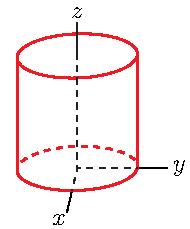
\includegraphics{cylinderA.pdf}\qquad
   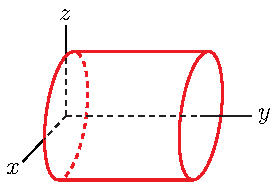
\includegraphics{cylinderB.pdf}
\end{center}
\end{efig}
\end{itemize}
\noindent
We have to compute the volume common to these two intersecting cylinders.

\begin{itemize}
\item
The equations $x^2+y^2=a^2$ and $x^2+z^2=a^2$ do not change at all 
if $x$ is replaced by $-x$. Consequently both cylinders, and hence our solid,
is symmetric about the $yz$-plane. In particular the volume of the
part of the solid in the octant $x\le 0$, $y\ge 0$, $z\ge 0$
is the same as the volume in the first octant $x\ge 0$, $y\ge 0$, $z\ge 0$.
Similarly, the equations do not change at all
if $y$ is replaced by $-y$ or if $z$ is replaced by $-z$. Our solid is
also symmetric about both the $xz$-plane and the $xy$-plane. 
Hence the volume of the part of our solid in each of the eight octants 
is the same.

\item So we will compute the volume of the part of 
the solid in the first octant, i.e. with $x\ge 0$, $y\ge 0$, $z\ge 0$.
The total volume of the solid is eight times that.

\end{itemize}
\noindent
The part of the solid in the first octant is sketched in the figure
on the left below. A point $(x,y,z)$ lies in the first cylinder
if and only if $x^2+y^2\le a^2$. 
\vadjust{
\begin{efig}
\begin{center}
   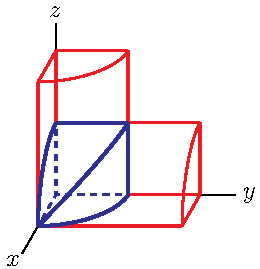
\includegraphics{cylinderC.pdf}\qquad\qquad
   \raisebox{0.1\height}{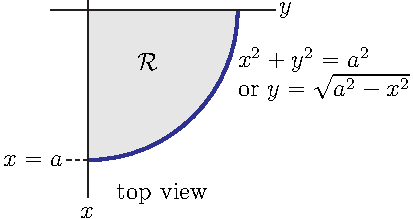
\includegraphics{cylinderD.pdf}}
\end{center}
\end{efig}
}
It lies in the second cylinder if and only if $x^2+z^2\le a^2$.
So the part of the solid in the first octant is
\begin{align*}
\cV_1&=\Set{(x,y,z)}{x\ge 0,\ y\ge 0,\ z\ge 0,\ x^2+y^2\le a^2,\ x^2+z^2\le a^2}
\end{align*}
Notice that, in $\cV_1$, $z^2\le a^2-x^2$ so that $z\le\sqrt{a^2-x^2}$ and
\begin{align*}
\cV_1
&=\Set{(x,y,z)}{x\ge 0,\ y\ge 0,\ x^2+y^2\le a^2,\ 0\le z\le \sqrt{a^2-x^2}}
\end{align*}
The top view of the part of the solid in the first octant is sketched 
in the figure on the right above. In that top view, $x$ runs from $0$
to $a$. For each fixed $x$, $y$ runs from $0$ to $\sqrt{a^2-x^2}$.
So we may rewrite
\begin{align*}
\cV_1=\Set{(x,y,z)}{(x,y)\in\cR,\ 0\le z\le f(x,y)}
\end{align*}
where
\begin{equation*}
\cR=\Big\{\ (x,y)\ \Big|\ 0\le x\le a,\ 0\le y\le \sqrt{a^2-x^2}\ \Big\}
\qquad\text{and}\qquad f(x,y) = \sqrt{a^2-x^2}
\end{equation*}
and ``$(x,y)\in\cR$'' is read ``$(x,y)$ is an element of $\cR$.''.
Note that $f(x,y)$ is actually independent of $y$. This will make things 
a bit easier below.

We can now compute the volume of $\cV_1$ using our usual abbreviated
protocol.
\begin{itemize}
\item
   Slice $\cR$ into long ``infinitesimally'' thin 
   horizontal strips of height $\dee{x}$.
\item
   Subdivide each strip into ``infinitesimal'' rectangles each of 
   width $\dee{y}$ and of height $\dee{x}$. See the figure below.
\begin{efig}
\begin{center}
   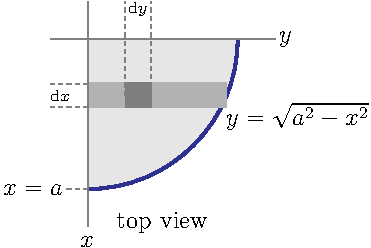
\includegraphics{cylinderE.pdf}
\end{center}
\end{efig}

\item
  The volume of the part of $\cV_1$ above rectangle centred on $(x,y)$
        is essentially 
   \begin{equation*}
       f(x,y)\,\dee{x}\,\dee{y}=\sqrt{a^2-x^2}\ \dee{x}\,\dee{y}
   \end{equation*}
\item 
   So the volume of the part of $\cV_1$ above the strip centred on $x$ is 
         essentially 
       \begin{equation*}
         \dee{x}\, \int_0^{\sqrt{a^2-x^2}} \sqrt{a^2-x^2}\ \dee{y}
       \end{equation*} 
   (the integral over $y$ adds up the volumes over all of the 
       different rectangles on the single horizontal strip in question) and  
\item
   we conclude that the
\begin{align*}
    \text{Volume}(\cV_1)
        &=\int_0^a \dee{x}\, \int_0^{\sqrt{a^2-x^2}}\dee{y}\ \sqrt{a^2-x^2}
\end{align*}
Here the integral over $x$ adds up the volumes over all 
of the different strips.
Recalling that, when integrating $y$, $x$ is held constant
\begin{align*}
\text{Volume}(\cV_1)
        &=\int_0^a \dee{x}\  \sqrt{a^2-x^2}\left[
                 \int_0^{\sqrt{a^2-x^2}} \dee{y} \right] \\
        &=\int_0^a \dee{x}\  \big(a^2-x^2\big) \\
        &=\left[a^2x-\frac{x^3}{3}\right]_0^a \\
        &=\frac{2a^3}{3}
\end{align*}
and the total volume of the solid in question is
\begin{equation*}
\text{Volume}(\cV)
=8\,\text{Volume}(\cV_1)
=\frac{16a^3}{3}
\end{equation*}
\end{itemize}

\end{eg}

\begin{eg}[Geometric Interpretation]\label{eg dblInt C}
Evaluate $\displaystyle\int_0^2\int_0^a \sqrt{a^2-x^2}\ \dee{x}\,\dee{y}$.

\soln This integral represents the volume of a simple geometric figure
and so can be evaluated without using any calculus at all.
The domain of integration is
\begin{equation*}
\cR=\Set{(x,y)}{0\le y\le 2,\  0\le x\le a}
\end{equation*}
and the integrand is $f(x,y) = \sqrt{a^2-x^2}$, so the integral 
represents the volume between the $xy$-plane and the surface 
$z=\sqrt{a^2-x^2}$, with $(x,y)$ running over $\cR$. We can rewrite 
the equation of the surface as $x^2+z^2=a^2$, which, as in 
Example \ref{eg dblInt B}, we recognize as the 
equation of a cylinder of radius $a$ centred on the $y$-axis.
We want the volume of the part of this cylinder that lies above
$\cR$. It is sketched in the figure below.
\begin{efig}
\begin{center}
   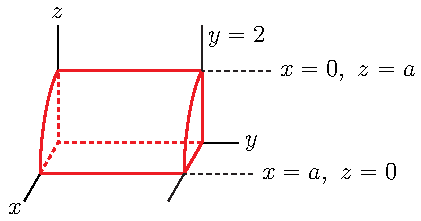
\includegraphics{qCylinder.pdf}\qquad\qquad
\end{center}
\end{efig}
The constant $y$ cross-sections of this volume are quarter
circles of radius $a$ and hence of area $\frac{1}{4}\pi a^2$. 
As $y$ runs from $0$ to $2$
\begin{equation*}
\int_0^2\int_0^a \sqrt{a^2-x^2}\ \dee{x}\,\dee{y}
=\frac{1}{4}\pi a^2\times 2
=\frac{\pi a^2}{2} 
\end{equation*}
\end{eg}

\begin{eg}[Example \ref{eg dblInt C}, the hard way]\label{eg dblInt CC}
It is possible, but very tedious, to evaluate the integral
$\int_0^2\int_0^a \sqrt{a^2-x^2}\ \dee{x}\,\dee{y}$
of Example \ref{eg dblInt C}, using single variable calculus
techniques. We do so now as a review of a couple of those
techniques.

The inside integral is $\int_0^a \sqrt{a^2-x^2}\ \dee{x}$.
The standard procedure for eliminating square roots like $\sqrt{a^2-x^2}$
from integrands is the method of trigonometric substitution, that was
covered in \S\eref{CLP101}{sec trigsub} of the CLP-2 text. In this
case, the appropriate substitution is
\begin{equation*}
x=a\sin\theta\qquad \dee{x}=a\cos\theta\ \dee{\theta}
\end{equation*} 
The lower limit of integration $x=0$, i.e. $a\sin\theta=0$, 
corresponds to $\theta=0$, and the upper limit  $x=a$, i.e. $a\sin\theta=a$, 
corresponds to $\theta=\frac{\pi}{2}$, so that
\begin{align*}
\int_0^a \sqrt{a^2-x^2}\ \dee{x}
&=\int_0^{\pi/2} \sqrt{\underbrace{a^2-a^2\sin^2\theta}_{a^2\cos^2\theta}}
        \ a\cos\theta\ \dee{\theta}
=a^2\int_0^{\pi2} \cos^2\theta\ \dee{\theta}
\end{align*}

The orthodox procedure for evaluating the resulting trigonometric integral
$\int_0^{\pi2} \cos^2\theta\ \dee{\theta}$, covered in 
\S\eref{CLP101}{sec trigint} of the CLP-2 text, uses the trigonometric
double angle formula
\begin{equation*}
\cos(2\theta) = 2\cos^2\theta -1\qquad\text{to write}\qquad
\cos^2\theta =\frac{1+\cos(2\theta)}{2}
\end{equation*}
and then
\begin{align*}
\int_0^a \sqrt{a^2-x^2}\ \dee{x}
&=a^2\int_0^{\pi2} \cos^2\theta\ \dee{\theta}
=\frac{a^2}{2} \int_0^{\pi/2} \big[1+\cos(2\theta)\big]\ \dee{\theta} \\
&=\frac{a^2}{2}\left[\theta+\frac{\sin(2\theta)}{2}\right]_0^{\pi/2} \\
&=\frac{\pi a^2}{4}
\end{align*}

However we remark that there is also an efficient, sneaky, way to evaluate
definite integrals like $\int_0^{\pi/2} \cos^2\theta\ \dee{\theta}$.
Looking at the figures 
\begin{mfig}
\begin{center}
    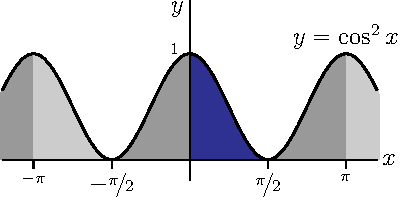
\includegraphics{cos2Agraph.pdf}\qquad
    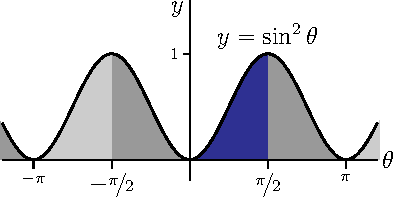
\includegraphics{sin2Agraph.pdf}
\end{center}
\end{mfig}
we see that 
\begin{equation*}
\int_0^{\pi/2} \cos^2\theta\ \dee{\theta}
=\int_0^{\pi/2} \sin^2\theta\ \dee{\theta}
\end{equation*}
Thus
\begin{align*}
\int_0^{\pi/2} \cos^2\theta\ \dee{\theta}
=\int_0^{\pi/2} \sin^2\theta\ \dee{\theta}
=\int_0^{\pi/2} \frac{1}{2}\big[\sin^2\theta+\cos^2\theta\big]\,\dee{\theta}
=\frac{1}{2}\int_0^{\pi/2} \dee{\theta}
=\frac{\pi}{4}
\end{align*}

In any event, the inside integral 
\begin{equation*}
\int_0^a \sqrt{a^2-x^2}\ \dee{x}
=\frac{\pi a^2}{4}
\end{equation*}
and the full integral
\begin{equation*}
\int_0^2\int_0^a \sqrt{a^2-x^2}\ \dee{x}\,\dee{y}
=\frac{\pi a^2}{4}\int_0^2\dee{y}
=\frac{\pi a^2}{2}
\end{equation*}
just as we saw in Example \ref{eg dblInt C}.
\end{eg}




\begin{eg}[ Order of Integration]\label{eg dblInt D}
The integral $\displaystyle\int_{-1}^2\int_{x^2}^{x+2}\dee{y}\,\dee{x}$
represents the area of a region in the $xy$-plane. Express the same area
as a double integral with the order on integration reversed.

\soln The critical step in reversing the order of integration is
to sketch the region in the $xy$-plane. Rewrite the given integral as
\begin{equation*}
\int_{-1}^2\int_{x^2}^{x+2}\dee{y}\,\dee{x}
=\int_{-1}^2\left[\int_{x^2}^{x+2}\dee{y}\right]\,\dee{x}
\end{equation*}
From this we see that, on the domain of integration,
\begin{itemize}
\item
$x$ runs from $-1$ to $2$ and
\item
for each fixed $x$, $y$ runs from the parabola $y=x^2$ to the straight line $y=x+2$.
\end{itemize}
The given iterated integral corresponds to the (vertical) slicing in the figure
on the left below.
\begin{wfig}
\begin{center}
   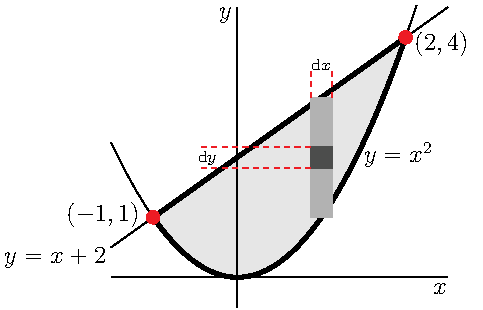
\includegraphics{reverseA.pdf}\ 
   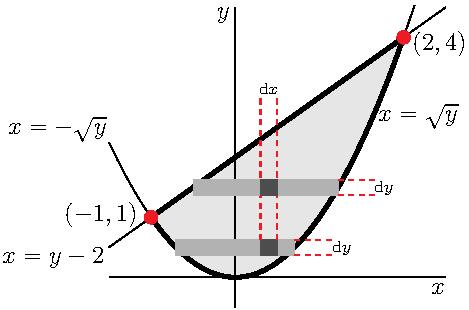
\includegraphics{reverseB.pdf}
\end{center}
\end{wfig}
To reverse the order of integration we have to switch to horizontal
slices as in the figure on the right above. 

There we see a new wrinkle:
the formula giving the value of $x$ at the left hand end of a slice
depends on whether the $y$ coordinate of the slice is bigger than, or smaller
than $y=1$. Looking at the figure on the right, we see that,
on the domain of integration,
\begin{itemize}
\item
$y$ runs from $0$ to $4$ and
\item
for each fixed $0\le y\le 1$, $x$ runs from $x=-\sqrt{y}$ to $x=+\sqrt{y}$.
\item
for each fixed $1\le y\le 4$, $x$ runs from $x=y-2$ to $x=+\sqrt{y}$.
\end{itemize} 
So
\begin{align*}
\int_{-1}^2\dee{x}\int_{x^2}^{x+2}\dee{y}
=\int_0^1\dee{y}\int_{-\sqrt{y}}^{\sqrt{y}}\dee{x}
  + \int_1^4\dee{y}\int_{y-2}^{\sqrt{y}}\dee{x}
\end{align*}
\end{eg}

There was a moral to the last example. Just because both orders of integration
have to give the same answer doesn't mean that they are equally easy to evaluate. Here is an extreme example illustrating that moral.

\begin{eg}\label{eg dblInt E}
Evaluate the integral of $\frac{\sin x}{x}$ over the region in the 
$xy$-plane that is above the $x$-axis, to the right of the line
$y=x$ and to the left of the line $x=1$. 

\soln Here is a sketch of the specified domain.
\begin{efig}
\begin{center}
   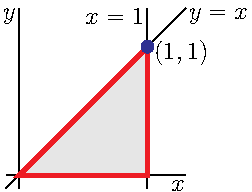
\includegraphics{reverse2A.pdf}
\end{center}
\end{efig}
We'll try to evaluate the specified integral twice --- once using
horizontal strips (the impossibly hard way) and once using 
vertical strips (the easy way).

\medskip\noindent\emph{Solution using horizontal strips.}\ \ \
To set up the integral using horizontal strips, as in the figure on
the left below, we observe that, on the domain of integration,
\begin{itemize}
\item
$y$ runs from $0$ to $1$ and
\item
for each fixed $y$, $x$ runs from $x=y$ to $1$.
\end{itemize}
So the iterated integral is
\begin{equation*}
\int_0^1\dee{y}\int_y^1\dee{x}\ \frac{\sin x}{x}
\end{equation*}
And we have a problem. The integrand $\frac{\sin x}{x}$ does not have
an antiderivative that can be expressed in terms of elementary 
functions\footnote{Perhaps the best known function whose antiderivative
cannot be expressed in terms of elementary functions is $e^{-x^2}$.
It is the integrand of the error function
$
\erf(x) =\frac{2}{\sqrt{\pi}}\int_0^x e^{-t^2}\ dt
$
that is used in computing ``bell curve'' probabilities. See Example
\eref{CLP101}{eg:erf} in the CLP-2 text.}.
It is impossible to evaluate $\int_y^1\dee{x}\ \frac{\sin x}{x}$ without
resorting to, for example, numerical methods or 
infinite series\footnote{See, for example,  
Example \eref{CLP101}{eg:erf} in the CLP-2 text.}.

\begin{efig}
\begin{center}
   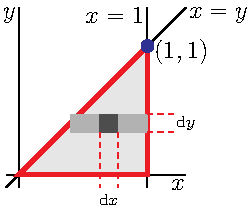
\includegraphics{reverse2B.pdf}\qquad
   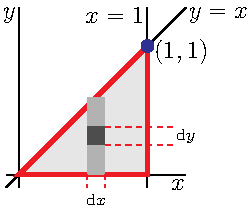
\includegraphics{reverse2C.pdf}
\end{center}
\end{efig}

\medskip\noindent\emph{Solution using vertical strips.}\ \ \
To set up the integral using vertical strips, as in the figure on
the right above, we observe that, on the domain of integration,
\begin{itemize}
\item
$x$ runs from $0$ to $1$ and
\item
for each fixed $x$, $y$ runs from $0$ to $y=x$.
\end{itemize}
So the iterated integral is
\begin{equation*}
\int_0^1\dee{x}\int_0^x\dee{y}\ \frac{\sin x}{x}
\end{equation*}
This time, because $x$ is treated as a constant in the inner integral,
it is trivial to evaluate the iterated integral.
\begin{align*}
\int_0^1\dee{x}\int_0^x\dee{y}\ \frac{\sin x}{x}
&=\int_0^1\dee{x}\ \frac{\sin x}{x}\int_0^x\dee{y}
=\int_0^1\dee{x}\ \sin x
=1-\cos 1
\end{align*}
\end{eg}

Here is an example which is included as an excuse to review
some integration technique from CLP-2. 
\begin{eg}\label{eg dblInt F}
Find the volume under the surface $z=1-3x^2-2y^2$ and above the $xy$-plane. 

\soln 
Before leaping into integration, we should try to understand what the surface
and volume look like.
For each constant $z_0$, the part of the surface $z=1-3x^2-2y^2$
that lies in the horizontal plane $z=z_0$ is the ellipse
$3x^2+2y^2=1-z_0$. The biggest of these ellipses is that in the
$xy$-plane, where $z_0=0$. It is the ellipse $3x^2+2y^2=1$.
As $z_0$ increases the ellipse shrinks, degenerating to a single
point, namely $(0,0,1)$, when $z_0=1$. So the surface consists 
of a stack of ellipses and our solid is
\begin{equation*}
\cV =\Set{(x,y,z)}{3x^2+2y^2\le 1,\ 0\le z\le 1-3x^2-2y^2}
\end{equation*}
This is sketched in the figure below
\begin{efig}
\begin{center}
   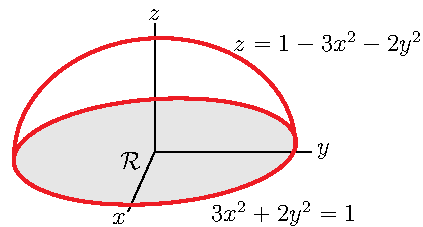
\includegraphics{egDblIntEa.pdf}
\end{center}
\end{efig}
The top view of the base region 
\begin{equation*}
\cR=\Set{(x,y)}{3x^2+2y^2\le 1}
\end{equation*}
is sketched in the figure below.
 \begin{efig}
\begin{center}
   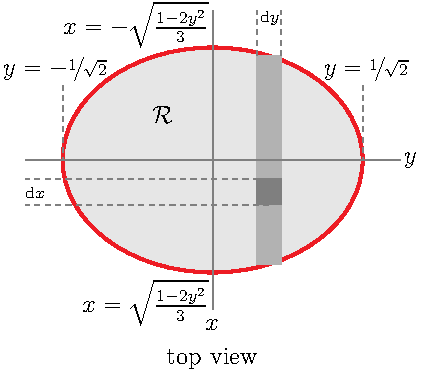
\includegraphics{egDblIntEb.pdf}
\end{center}
\end{efig}

Considering that the $x$-dependence in $z=1-3x^2-2y^2$
is almost identical to the $y$-dependence in $z=1-3x^2-2y^2$
(only the coefficients $2$ and $3$ are interchanged), using
vertical slices is likely to lead to exactly the same level of difficulty
as using horizontal slices. So we'll just pick one --- say vertical
slices.

The fattest part of $\cR$ is on the $y$-axis. The intersection
points of the ellipse with the $y$-axis have $x=0$ and $y$
obeying $3(0)^2+2y^2 =1 $ or $y=\pm\nicefrac{1}{\sqrt{2}}$. So
in $\cR$, $-\nicefrac{1}{\sqrt{2}}\le y\le \nicefrac{1}{\sqrt{2}}$
and, for each such $y$, $3x^2\le 1-2y^2$ or 
$-\sqrt{\frac{1-2y^2}{3}}\le x\le \sqrt{\frac{1-2y^2}{3}}$.
So using vertical strips as in the figure above
\begin{align*}
\text{Volume}(\cV) &=\dblInt_\cR \big(1-3x^2-2y^2\big)\,\dee{x}\,\dee{y} \\
   &=\int_{-\nicefrac{1}{\sqrt{2}}}^{\nicefrac{1}{\sqrt{2}}}\dee{y}
     \int_{-\sqrt{\frac{1-2y^2}{3}}}^{\sqrt{\frac{1-2y^2}{3}}}\dee{x}\ 
             \big(1-3x^2-2y^2\big) \\
   &=4\int_0^{\nicefrac{1}{\sqrt{2}}}\dee{y}
      \int_0^{\sqrt{\frac{1-2y^2}{3}}}\dee{x}\ 
             \big(1-3x^2-2y^2\big) \\
   &=4\int_0^{\nicefrac{1}{\sqrt{2}}}\dee{y}\ 
             \Big[(1-2y^2)x-x^3\Big]_0^{\sqrt{\frac{1-2y^2}{3}}} \\
   &=4\int_0^{\nicefrac{1}{\sqrt{2}}}\dee{y}\ 
             \sqrt{\frac{1-2y^2}{3}}\ \Big[(1-2y^2)-\frac{1-2y^2}{3}\Big] \\
   &=8\int_0^{\nicefrac{1}{\sqrt{2}}}\dee{y}\ 
             \left[\frac{1-2y^2}{3}\right]^{3/2} 
\end{align*}
To evaluate this integral, we use the trig 
substitution\footnote{See \S\eref{CLP101}{sec trigsub} in the CLP-2 text
for a general discussion of trigonometric substitution.}
$2y^2=\sin^2\theta$, or 
\begin{equation*}
y=\frac{\sin\theta}{\sqrt{2}}\qquad
\dee{y}=\frac{\cos\theta}{\sqrt{2}}\,\dee{\theta}
\end{equation*}
to give
\begin{align*} 
\text{Volume}(\cV) &= 8\int_0^{\nicefrac{\pi}{2}}
          \overbrace{\dee{\theta}\ \frac{\cos\theta}{\sqrt{2}} }^{\dee{y}}
           \left[\frac{\cos^2\theta}{3}\right]^{3/2} 
    =\frac{8}{\sqrt{54}}\int_0^{\nicefrac{\pi}{2}}\dee{\theta}\ 
                      \cos^4\theta
\end{align*}
Then to integrate $\cos^4\theta$, we use the double angle 
formula\footnote{We weren't joking about his being a good review of
single variable integration techniques. See Example \eref{CLP101}{eg:TRGINTc} 
in the CLP-2 text.}
\begin{align*}
\cos^2\theta &=\frac{\cos(2\theta)+1}{2} \\
\implies \cos^4\theta &= \frac{\big(\cos(2\theta)+1\big)^2}{4}
    =\frac{\cos^2(2\theta)+2\cos(2\theta)+1}{4}
    =\frac{\frac{\cos(4\theta)+1}{2}+2\cos(2\theta)+1}{4} \\
   &=\frac{3}{8} +\frac{1}{2}\cos(2\theta) +\frac{1}{8}\cos(4\theta)
\end{align*}
Finally, since $\int_0^{\nicefrac{\pi}{2}} \cos(4\theta)\,\dee{\theta}
               =\int_0^{\nicefrac{\pi}{2}} \cos(2\theta)\,\dee{\theta}
               =0$,
\begin{align*}
\text{Volume}(\cV) = \frac{8}{\sqrt{54}}\ \frac{3}{8}\ \frac{\pi}{2}
  =\frac{\pi}{2\sqrt{6}}
\end{align*}


\end{eg}

%%%%%%%%%%%%%%%%%%%%%%%%%%%%%%%%%%%%%%%%%%%%%%%%%%
\subsection{Optional --- More about the Definition of 
$\ \dblInt_\cR f(x,y)\ \dee{x}\dee{y}$}
\label{sec def int more}
%%%%%%%%%%%%%%%%%%%%%%%%%%%%%%%%%%%%%%%%%%%%%%%%

Technically, the integral $\dblInt_\cR f(x,y)\ \dee{x}\,\dee{y}$, where 
$\cR$ is a bounded region in $\bbbr^2$, is defined as follows. 

\begin{itemize}
\item
Subdivide $\cR$ by drawing lines parallel to the $x$ and $y$ axes.
\begin{efig}
\begin{center}
   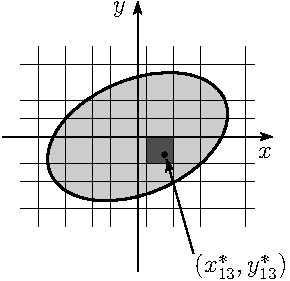
\includegraphics{intDecomp2.pdf}
\end{center}
\end{efig}

\item
Number the resulting rectangles contained in $\cR$, $1$ through $n$.
Notice that we are numbering all of the rectangles in $\cR$, not just those 
in one particular row or column.
\item
Denote by $\De A_i$ the area of rectangle $\# i$.
\item
Select an arbitrary point $(x_i^*,y_i^*)$ in rectangle $\# i$.
\item
Form the sum $\sum\limits_{i=1}^n f(x_i^*,y_i^*) \De A_i $.
Again note that the sum runs over all of the rectangles in $\cR$, 
not just those  in one particular row or column.
\end{itemize}
\noindent 
Now repeat this construction over and over again, using finer and 
finer grids. If, as the size\footnote{For example, let $p_i$ be the perimeter 
of rectangle number $i$ and require that $\max_{1\le i\le n} p_i$ tends
to zero. This way both the heights and widths of all rectangles 
also tend to zero.} of the rectangles approaches zero, 
this sum approaches a unique limit (independent of the choice
of parallel lines and of points $(x_i^*,y_i^*)$),  then we define
\begin{equation*}
\dblInt_\cR f(x,y)\ \dee{x}\,\dee{y}
   =\lim \sum_{i=1}^n f(x_i^*,y_i^*)\,\De A_i
\end{equation*}

\begin{theorem}
If $f(x,y)$ is continuous in a region $\cR$ described by
\begin{alignat*}{3}
a&\le x&&\le b \\
B(x)&\le y&&\le T(x)
\end{alignat*}
for continuous functions $B(x)$, $T(x)$, then
\begin{equation*}
\dblInt_\cR f(x,y)\ \dee{x}\,\dee{y}\qquad\text{and}\qquad
\int_a^b \dee{x} \bigg[\int_{B(x)}^{T(x)}\dee{y}\  f(x,y)\bigg]
\end{equation*}
both exist and are equal. 
Similarly, if $\cR$ is described by
\begin{alignat*}{3}
c&\le y&&\le d\\
L(y)&\le x&&\le R(y)
\end{alignat*}
for continuous functions $L(y)$, $R(y)$, then
\begin{equation*}
\dblInt_R f(x,y)\ \dee{x}\,\dee{y}\qquad\text{and}\qquad
\int_c^d \dee{y} \bigg[\int_{L(y)}^{R(y)}\dee{x}\  f(x,y)\bigg]
\end{equation*}
both exist and are equal.
\end{theorem}


The proof of this theorem is not particularly difficult, but is still 
beyond the scope of this text. The main ideas in the proof can already
be seen in section \eref{CLP101}{ssec careful defn} of the CLP-2 text.
An important consequence of this theorem is
\begin{theorem}[Fubini]
If $f(x,y)$ is continuous in a region $\cR$ described by both
%\begin{alignat*}{3}
%a&\le x&&\le b \\
%B(x)&\le y&&\le T(x)
%\end{alignat*}
%and
%\begin{alignat*}{3}
%c&\le y&&\le d\\
%L(y)&\le x&&\le R(y)
%\end{alignat*}
\begin{equation*}
\left\{\begin{aligned}
   a&\le x\le b \\
B(x)&\le y\le T(x)
\end{aligned}\right\}
\qquad\text{and}\qquad
\left\{
\begin{aligned}
c&\le y\le d\\
L(y)&\le x\le R(y)
\end{aligned}
\right\}
\end{equation*}
for continuous functions $B(x)$, $T(x)$, $L(y)$, $R(y)$, then
both
\begin{equation*}
\int_a^b \dee{x} \bigg[\int_{B(x)}^{T(x)}\dee{y}\  f(x,y)\bigg]
\qquad\text{and}\qquad
\int_c^d \dee{y} \bigg[\int_{L(y)}^{R(y)}\dee{x}\  f(x,y)\bigg]
\end{equation*}
exist and are equal.
\end{theorem}

The hypotheses of both of these theorems can be relaxed a bit, but not
too much. For example, if
\begin{equation*}
\cR=\Set{(x,y)}{0\le x\le 1,\ 0\le y\le 1}\qquad
f(x,y)=\begin{cases}
           1&\text{if $x$, $y$ are both rational numbers} \\
           0&\text{otherwise}
      \end{cases}
\end{equation*}
then the integral $\dblInt_\cR f(x,y)\ \dee{x}\,\dee{y}$ does not exist. This
is easy to see. If all of the $x_i^*$'s and $y_i^*$'s are chosen to be rational
numbers, then
\begin{equation*}
\sum_{i=1}^n f(x_i^*,y_i^*)\,\De A_i
=\sum_{i=1}^n \,\De A_i
=\text{Area}(\cR)
\end{equation*}
But if we choose all  the $x_i^*$'s and $y_i^*$'s to be irrational numbers, then
\begin{equation*}
\sum_{i=1}^n f(x_i^*,y_i^*)\,\De A_i
=\sum_{i=1}^n 0\,\De A_i
=0
\end{equation*}
So the limit of $\sum\limits_{i=1}^n f(x_i^*,y_i^*)\,\De A_i$, 
as the maximum diagonal of the rectangles approaches zero,
depends on the choice of points $(x_i^*,y_i^*)$. So the integral
$\dblInt_\cR f(x,y)\ \dee{x}\,\dee{y}$ does not exist.

Here is an even more pathological\footnote{For mathematicians, ``pathological'' is a synonym for ``cool''.} example. 
\begin{eg}\label{eg bad Fubini}
In this example, we relax 
exactly one of the hypotheses of Fubini's Theorem, namely the continuity 
of $f$, and construct an example in which both of the integrals in 
Fubini's Theorem exist, but are \textbf{not equal}. In fact,
we choose $\cR=\Set{(x,y)}{0\le x\le 1,\ 0\le y\le 1}$ and we use a function
$f(x,y)$ that is continuous on $\cR$, except at exactly one point --- 
the origin.


First, let $\de_1,\de_2,\de_3,\ \cdots$ be any sequence of real numbers
obeying 
$$
1=\de_1>\de_2>\de_3,\ \cdots,\ \de_n\rightarrow 0
$$ 
For example $\de_n=\frac{1}{n}$ or $\de_n=\frac{1}{2^{n-1}}$ are both
acceptable.
For each positive integer $n$, let 
$I_n=(\de_{n+1},\de_n]=\Set{t}{\de_{n+1}<t\le \de_n}$ and
let $g_n(t)$ be any nonnegative continuous function obeying 
\begin{itemize}
\item
$g_n(t)=0$ if $t$ is not in $I_n$ 
and 
\item
$\int_{I_n}g(t)\,dt=1$
\end{itemize}
There are many such functions. For example
\begin{equation*}
g_n(t)=\frac{2}{\de_n-\de_{n+1}}\begin{cases}
   \de_n-t& \text{if $\half(\de_{n+1}+\de_n)\le t\le \de_n$}\\[0.05in]
   t-\de_{n+1}& \text{if $\de_{n+1}\le t\le \half(\de_{n+1}+\de_n)$}\\[0.05in]
   0& \text{otherwise}
   \end{cases}\qquad\raisebox{-45pt}[42pt][52pt]{\includegraphics{g_n}}
\end{equation*}
Here is a summary of what we have done so far.
\begin{itemize}
\item
We subdivided the interval $0< x\le 1$ into infinitely many subintervals
$I_n$. As $n$ increases, the subinterval $I_n$ gets smaller and smaller and
also gets closer and closer to zero.
\item  
We defined, for each $n$, a nonnegative continuous function $g_n$ 
that is zero everywhere outside of $I_n$ and whose integral over $I_n$ is one.
\end{itemize}


Now we define the integrand $f(x,y)$ in terms of these subintervals $I_n$
and functions $g_n$.
\begin{equation*}
f(x,y)=\begin{cases}
   0& \text{if $x=0$}\\[0.05in]
   0& \text{if $y=0$}\\[0.05in]
   g_m(x)g_n(y)& \text{if $x\in I_m,\ y\in I_n$ with $m=n$}\\[0.05in]
   -g_m(x)g_n(y)& \text{if $x\in I_m,\ y\in I_n$ with $m=n+1$}\\[0.05in]
   0& \text{otherwise}
   \end{cases}
\end{equation*}
You should think of $(0,1]\times(0,1]$ as a union of a bunch of 
small rectangles $I_m\times I_n$, as in the figure below. On most 
of these rectangles, $f(x,y)$ is just zero. The exceptions are the 
darkly shaded rectangles $I_n\times I_n$ on the ``diagonal'' of the figure 
and the lightly shaded rectangles $I_{n+1}\times I_n$ just to the left 
of the ``diagonal''. 

On each darkly shaded rectangle, $f(x,y)\ge 0$ and the graph of $f(x,y)$ 
is the graph of $g_n(x)g_n(y)$ which looks like a pyramid. On each 
lightly shaded rectangle, $f(x,y)\le 0$ and the graph of $f(x,y)$ is 
the graph of $-g_{n+1}(x)g_n(y)$ which looks like a pyramidal hole 
in the ground. 
\begin{figure}[h]
\begin{efig}
\begin{center}
   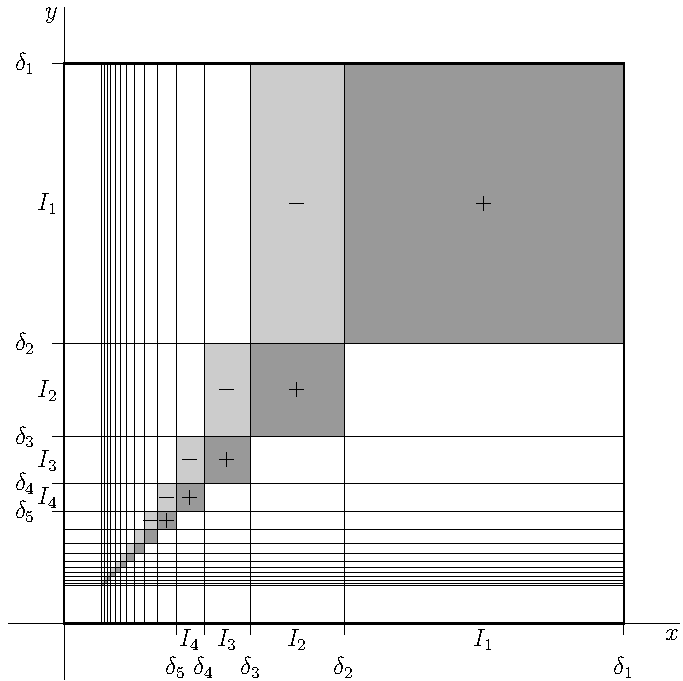
\includegraphics[scale=0.8]{fubini.pdf}
\end{center}
\end{efig}
\end{figure}

Now fix any $0\le y\le 1$ and let's compute $\int_0^1 f(x,y)\ \dee{x}$.
That is, we are integrating $f$ along a line that is parallel to the $x$-axis.
If $y=0$, then $f(x,y)=0$ for all $x$, so $\int_0^1 f(x,y)\,\dee{x}~=~0$.
If $0<y\le 1$, then there is exactly one positive integer $n$ with 
$y\in I_n$ and $f(x,y)$ is zero, except for $x$ in $I_n$ or $I_{n+1}$. 
So for $y\in I_n$
\begin{align*}
\int_0^1 f(x,y)\,\dee{x}&=\sum_{m=n,n+1}\int_{I_m} f(x,y)\,\dee{x}
=\int_{I_n} g_n(x)g_n(y)\,\dee{x}-\int_{I_{n+1}} g_{n+1}(x)g_n(y)\,\dee{x} \\
&=g_n(y)\int_{I_n} g_n(x)\,\dee{x}-g_n(y)\int_{I_{n+1}} g_{n+1}(x)\,\dee{x} \\
&=g_n(y)-g_n(y)=0
\end{align*}
Here we have twice used that $\int_{I_m}g(t)\,dt=1$ for all $m$. Thus
$\int_0^1 f(x,y)\,\dee{x}=0$ for all $y$ and hence $\int_0^1\dee{y}\Big[\int_0^1
\dee{x}\ f(x,y)\Big]=0$.

Finally, fix any $0\le x\le 1$ and let's compute $\int_0^1 f(x,y)\ \dee{y}$.
That is, we are integrating $f$ along a line that is parallel to the $y$-axis.
If $x=0$, then $f(x,y)=0$ for all $y$, so $\int_0^1 f(x,y)\,\dee{y}~=~0$.
If $0<x\le 1$, then there is exactly one positive integer $m$ with 
$x\in I_m$. If $m\ge 2$, then $f(x,y)$ is zero, except for $y$ in $I_m$ and 
$I_{m-1}$. But, if $m=1$, then $f(x,y)$ is zero, except for $y$ in $I_1$.
(Take another look at the figure above.) 
So for $x\in I_m$, with $m\ge 2$,
\begin{align*}
\int_0^1 f(x,y)\,\dee{y}&=\sum_{n=m,m-1}\int_{I_n} f(x,y)\,\dee{y}
=\int_{I_m} g_m(x)g_m(y)\,\dee{y}-\int_{I_{m-1}} g_{m}(x)g_{m-1}(y)\,\dee{y} \\
&=g_m(x)\int_{I_m} g_m(y)\,\dee{y}-g_m(x)\int_{I_{m-1}} g_{m-1}(y)\,\dee{y} \\
&=g_m(x)-g_m(x)=0
\end{align*}
But for $x\in I_1$,
\begin{align*}
\int_0^1 f(x,y)\,\dee{y}&=\int_{I_1} f(x,y)\,\dee{y}
=\int_{I_1} g_1(x)g_1(y)\,\dee{y}
=g_1(x)\int_{I_1} g_1(y)\,\dee{y}
=g_1(x)
\end{align*}
 Thus
\begin{equation*}
\int_0^1 f(x,y)\,\dee{y}=\begin{cases}
                          0&\text{if $x\le \de_2$} \\
                         g_1(x)&\text{if $x\in I_1$}
                          \end{cases}
\end{equation*}
and hence
\begin{equation*}
\int_0^1\dee{x}\bigg[\int_0^1 \dee{y}\ f(x,y)\bigg]
=\int_{I_1}g_1(x)\,\dee{x}=1
\end{equation*}
The conclusion is that for the $f(x,y)$ above, which is defined 
for all $0\le x\le 1$, $0\le y\le 1$ and is continuous except at $(0,0)$,
\begin{equation*}
\int_0^1\dee{y}\bigg[\int_0^1 \dee{x}\ f(x,y)\bigg]=0
\qquad
\int_0^1\dee{x}\bigg[\int_0^1 \dee{y}\ f(x,y)\bigg]=1
\end{equation*}
\end{eg}

%%%%%%%%%%%%%%%%%%%%%%%%%%%%%%%%%%%%%%%%%%%%%%%%%%
\section{Double Integrals in Polar Coordinates} \label{sec polars}
%%%%%%%%%%%%%%%%%%%%%%%%%%%%%%%%%%%%%%%%%%%%%%%%
So far, in setting up integrals, we have always cut up the
domain of integration into tiny rectangle by drawing in many lines
of constant $x$ and many lines of constant $y$.
\begin{efig}
\begin{center}
   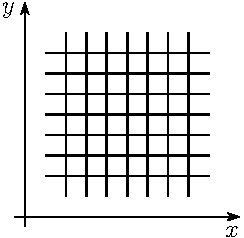
\includegraphics{intDecomp3.pdf}
\end{center}
\end{efig}
There is no law that says that we must cut up our domains of integration
into tiny pieces in that way. Indeed, when the objects of interest
are sort of round and centered on the origin, it is often 
advantageous\footnote{The ``golden hammer'' (also known as Maslow's hammer
and as the law of the instrument) refers to a tendency to always use 
the same tool, even when it isn't the best tool for the job.
It is just as bad in mathematics as it is in carpentry.} 
to use polar coordinates, rather than Cartesian coordinates. 


%%%%%%%%%%%%%%%%%%%%%%%%%%%%%%%%%%%%%%%%%%%%%%%%%%
\subsection{Polar Coordinates} \label{sec polar coords}
%%%%%%%%%%%%%%%%%%%%%%%%%%%%%%%%%%%%%%%%%%%%%%%%
It may have been a while since you did anything in polar coordinates.
So let's review before we resume integrating.
%First, here is a review of the definition of polar coordinates.
\begin{defn}\label{def polars}
The polar coordinates\footnote{In the mathematical literature,
the angular coordinate is usually denoted $\theta$, as we do here.
The symbol $\varphi$ is also often used for the angular coordinate.
In fact there is an ISO standard (\#31--11) which specifies 
that $\varphi$ should be used in the natural sciences and in technology.} 
of any point $(x,y)$ in the $xy$-plane are
\begin{align*}
r&=\text{ the distance from }(0,0)\text{ to }(x,y)\\
\theta&=\text{ the (counter-clockwise) angle between the $x$ axis 
               and the line joining $(x,y)$ to $(0,0)$}
\end{align*}
\begin{efig}
\begin{center}
    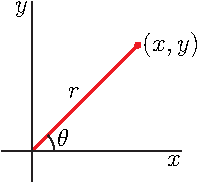
\includegraphics{polar.pdf}
\end{center}
\end{efig}
\end{defn}
Cartesian and polar coordinates are related, via a quick bit
of trigonometry, by
\begin{impeqn}\label{eqn polars}
\begin{align*}
x&=r\cos\theta &
y&=r\sin\theta  \\
    r&=\sqrt{x^2+y^2} &
    \theta&=\arctan\frac{y}{x}
\end{align*}
\end{impeqn}
The following two figures show a number of lines of constant $\theta$,
on the left, and curves of constant $r$, on the right.
\begin{efig}
\begin{center}
    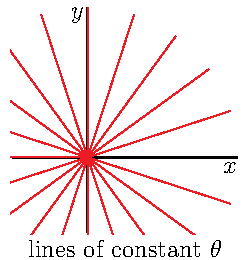
\includegraphics{polarTh.pdf}\qquad\qquad
    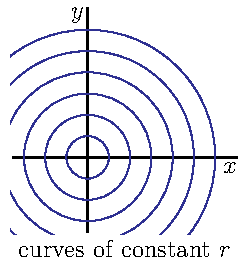
\includegraphics{polarR.pdf}
\end{center}
\end{efig}


Note that the polar angle $\theta$ is only defined up to integer multiples
of $2\pi$. For example, the point $(1,0)$ on the $x$-axis could have 
$\theta=0$, but could also have $\theta=2\pi$ or $\theta=4\pi$. It is sometimes
convenient to assign $\theta$ negative values. When $\theta<0$, the
counter-clockwise\footnote{or anti-clockwise or widdershins.
Yes, widdershins is a real word, though the Oxford English Dictionary
lists its frequency of usage as between 0.01 and 0.1 times
per million words. Of course both ``counter-clockwise''
and ``anti-clockwise'' assume that your clock is not a sundial in the
southern hemisphere.} 
angle $\theta$ refers to the clockwise angle $|\theta|$. For example,
the point $(0,-1)$ on the negative $y$-axis can have $\theta=-\frac{\pi}{2}$
and can also have $\theta=\frac{3\pi}{2}$.\begin{efig}
\begin{center}
    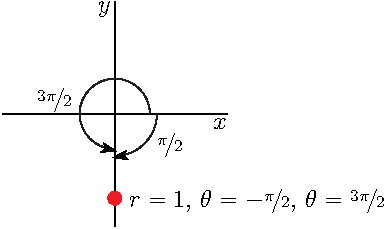
\includegraphics{polarNegTh.pdf}
\end{center}
\end{efig}



It is also sometimes convenient to extend the above definitions by saying that
$x=r\cos\theta$ and $y=r\sin\theta$ even when $r$ is negative. For example,
the following figure shows $(x,y)$ for $r=1$, $\theta=\nicefrac{\pi}{4}$
and for $r=-1$, $\theta=\nicefrac{\pi}{4}$.
\vadjust{
\begin{efig}
\begin{center}
    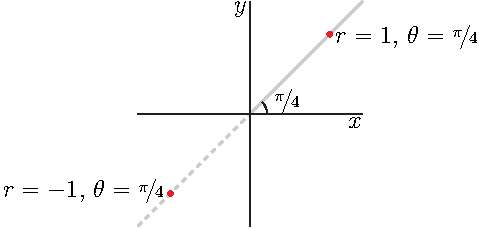
\includegraphics{polarNeg.pdf}
\end{center}
\end{efig}
}
Both points lie on the  line through the origin that makes an angle of
$45^\circ$ with the $x$-axis and both are a distance one from the origin.
But they are on opposite sides of the the origin.


%%%%%%%%%%%%%%%%%%%%%%%%%%%%%%%%%%%%%%%%%%%%%%%%%%
\subsection{Polar Curves} \label{sec polar curves}
%%%%%%%%%%%%%%%%%%%%%%%%%%%%%%%%%%%%%%%%%%%%%%%%

Here are a couple of examples in which we sketch curves specified 
by equations in terms of polar coordinates.

\begin{eg}[The Cardioid]\label{eg cardioid}
Let's sketch the curve 
\begin{equation*}
r= 1+\cos\theta
\end{equation*}
Our starting will be to understand how $1+\cos\theta$ varies with $\theta$.
So it will be helpful to 
remember what the graph of $\cos\theta$ looks like for $0\le\theta\le 2\pi$.
\begin{efig}
\begin{center}
    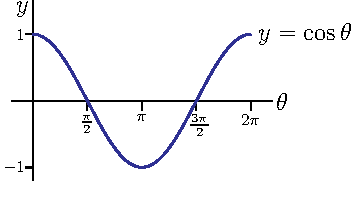
\includegraphics{cosGraph.pdf}
\end{center}
\end{efig}
From this we see that the graph of $y=1+\cos\theta$ is 
\begin{efig}
\begin{center}
    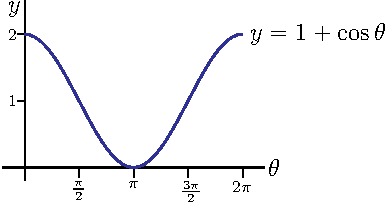
\includegraphics{cosGraphP1.pdf}
\end{center}
\end{efig}
Now let's pick some easy $\theta$ values, find the corresponding $r$'s
and sketch them.

\begin{itemize}
\item 
When $\theta=0$, we have $r=1+\cos 0 = 1+1=2$. To sketch the
point with $\theta=0$ and $r=2$, we first draw in the half-line consisting 
of all points with $\theta=0$, $r>0$. That's the positive $x$-axis, 
sketched in gray in the leftmost figure below. Then we put in a dot on that line
a distance $2$ from the origin. That's the red dot in the leftmost figure below.
\item
Now increase $\theta$ a bit (to another easy place to evaluate), 
say to $\theta=\frac{\pi}{6}$.
As we do so $r=1+\cos\theta$ decreases to 
$r=1+\cos\frac{\pi}{6} = 1+\frac{\sqrt{3}}{2}\approx 1.87$.
To sketch the point with $\theta=\frac{\pi}{6}$ and $r\approx 1.87$, 
we first draw in the half-line consisting of all points with $\theta=\frac{\pi}{6}$, $r>0$. 
That's the upper gray line in the second figure below.
Then we put in a dot on that line a distance $1.87$ from the origin. 
That's the upper red dot in the second figure below.
\begin{efig}
\begin{center}
    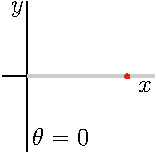
\includegraphics{cardioid1.pdf}\qquad\qquad
    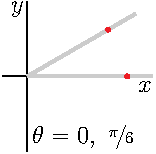
\includegraphics{cardioid2.pdf}\qquad\qquad
    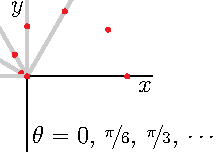
\includegraphics{cardioid3.pdf}
\end{center}
\end{efig}

\item
Now increase $\theta$ still more, say to 
    \begin{itemize}\itemsep1pt \parskip0pt \parsep0pt
        \item
          $\theta=\frac{2\pi}{6}=\frac{\pi}{3}$,
        \item
          followed by $\theta=\frac{3\pi}{6}=\frac{\pi}{2}$, 
        \item
          followed by $\theta=\frac{4\pi}{6}=\frac{2\pi}{3}$,
        \item
          followed by $\theta=\frac{5\pi}{6}$,
        \item
          followed by $\theta=\frac{6\pi}{6}=\pi$.
   \end{itemize}          
As $\theta$ increases, $r=1+\cos\theta$ decreases, hitting $r=1$ when 
$\theta=\frac{\pi}{2}$ and ending at $r=0$ when $\theta=\pi$.
For each of these $\theta$'s,  we first draw in the half-line consisting 
of all points with that $\theta$ and $r\ge 0$. 
Those are the five gray lines in the figure on the right above.
Then we put in a dot on each $\theta$-line a distance $r=1+\cos\theta$ 
from the origin. Those are the red dots on the gray lines in the 
figure on the right above.

\item 
We could continue the above procedure for $\pi\le\theta\le 2\pi$.
Or we can look at the graph of $\cos\theta$ above and notice that
the graph of $\cos\theta$ for $\pi\le\theta\le 2\pi$
is exactly the mirror image, about $\theta=\pi$, of the graph of $\cos\theta$
for $0\le\theta\le \pi$. 
\vadjust{
\begin{efig}
\begin{center}
    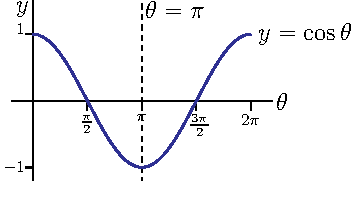
\includegraphics{cosGraphR.pdf}
\end{center}
\end{efig}
}
That is, $\cos(\pi+\theta) =\cos(\pi-\theta)$
so that $r(\pi+\theta) = r(\pi-\theta)$. So we get the figure.
\begin{efig}
\begin{center}
    \includegraphics{cardiod4.pdf}
\end{center}
\end{efig}

\item
Finally, we fill in a smooth curve through the dots and we get the
graph below. This curve is called a \emph{cardiod} because it looks
like a heart\footnote{Well, a mathematician's heart. The name ``cardioid''
comes from the Greek word $\kappa \alpha \rho \delta \iota \alpha$
(which anglicizes to kardia) for heart.}.
\begin{efig}
\begin{center}
    \includegraphics{cardiodF.pdf}
\end{center}
\end{efig}
\end{itemize}
\end{eg}


\begin{eg}[The Three Petal Rose]\label{eg rose}
Now we'll use the same procedure as in the last example to sketch
the graph of 
\begin{equation*}
r=\sin(3\theta)
\end{equation*}
Again it will be useful to remember 
what the graph of $\sin(3\theta)$ looks like for $0\le\theta\le 2\pi$.
\begin{efig}
\begin{center}
    \includegraphics{sin3Graph.pdf}
\end{center}
\end{efig}
\begin{itemize}
\item 
We'll first consider $0\le\theta\le\frac{\pi}{3}$, so that
$0\le 3\theta \le \pi$. On this interval $r(\theta)=\sin(3\theta)$
   \begin{itemize}\itemsep1pt \parskip0pt \parsep0pt
        \item
          starts with $r(0)=0$, and then
        \item
          increases as $\theta$ increases until
        \item
         $3\theta=\frac{\pi}{2}$, i.e. $\theta=\frac{\pi}{6}$,
          where $r\big(\nicefrac{\pi}{6}\big)=1$, and then
        \item
          decreases as $\theta$ increases until
        \item
         $3\theta=\pi$, i.e. $\theta=\frac{\pi}{3}$,
          where $r\big(\nicefrac{\pi}{3}\big)=0$, again.
   \end{itemize}  
Here is a table giving a few values of $r(\theta)$ for 
  $0\le \theta\le\frac{\pi}{3}$. Notice that we have chosen values of 
$\theta$ for which $\sin(3\theta)$ is easy to compute.

\begin{center}
     \renewcommand{\arraystretch}{1.3}
     \begin{tabular}{ | c | c | c |}
     \hline
     $\theta$ & $3\theta$ & $r(\theta)$ \\
      \hline
      0        &     0     &    0      \\
      \hline
      $\nicefrac{\pi}{12}$  & $\nicefrac{\pi}{4}$  & 
                  $\nicefrac{1}{\sqrt{2}}\approx  0.71$   \\
     \hline
      $\nicefrac{2 \pi}{12}$  & $\nicefrac{\pi}{2}$  &  $1$   \\
      \hline
      $\nicefrac{3 \pi}{12}$  & $\nicefrac{3\pi}{4}$  & 
                  $\nicefrac{1}{\sqrt{2}}\approx  0.71$   \\
     \hline
      $\nicefrac{4 \pi}{12}$  & $\pi$  &  $0$   \\
     \hline
     \end{tabular}
     \renewcommand{\arraystretch}{1.0}
\end{center}
and here is a sketch exhibiting those values and another sketch of the
part of the curve with $0\le \theta\le\frac{\pi}{3}$.
\begin{efig}
\begin{center}
    \includegraphics{rose1.pdf}\qquad\qquad
    \includegraphics{rose1b.pdf}
\end{center}
\end{efig}

\item 
Next consider $\frac{\pi}{3}\le\theta\le\frac{2\pi}{3}$, so that
$\pi\le 3\theta \le 2\pi$. On this interval $r(\theta)=\sin(3\theta)$
   \begin{itemize}\itemsep1pt \parskip0pt \parsep0pt
        \item
          starts with $r\big(\nicefrac{\pi}{3}\big)=0$, and then
        \item
          decreases as $\theta$ increases until
        \item
         $3\theta=\frac{3\pi}{2}$, i.e. $\theta=\frac{\pi}{2}$,
          where $r\big(\nicefrac{\pi}{2}\big)=-1$, and then
        \item
          increases as $\theta$ increases until
        \item
         $3\theta=2\pi$, i.e. $\theta=\frac{2\pi}{3}$,
          where $r\big(\nicefrac{2\pi}{3}\big)=0$, again.
   \end{itemize}  
We are now encountering, for the first time, $r(\theta)$'s that are negative.
The figure on the left below contains, for each of 
$\theta = \frac{4\pi}{12}=\frac{\pi}{3}$, $\frac{5\pi}{12}$, 
$\ \frac{6\pi}{12}=\frac{\pi}{2}$, $\ \frac{7\pi}{12}$ and 
$\ \frac{8\pi}{12}=\frac{2\pi}{3}$
   \begin{itemize}\itemsep1pt \parskip0pt \parsep0pt
        \item
          the (dashed) half-line consisting of all points with that 
           $\theta$ and $r<0$ and
        \item
           the dot with that $\theta$ and $r(\theta)=\sin(3\theta)$.      
   \end{itemize} 
The figure on the right below provides a sketch of the
part of the curve $r=\sin(3\theta)$ with 
$\frac{\pi}{3}\le \theta\le \frac{2\pi}{3}$. 
\begin{efig}
\begin{center}
    \includegraphics{rose2.pdf}\qquad\qquad
    \includegraphics{rose2b.pdf}
\end{center}
\end{efig}

\item 
Finally consider $\frac{2\pi}{3}\le\theta\le\pi$ (because
$r(\theta+\pi) = \sin (3\theta+3\pi) = -\sin(3\theta)=-r(\theta)$,
the part of the curve with $\pi\le\theta\le 2\pi$ just retraces
the part with $0\le\theta\le \pi$), so that
$2\pi\le 3\theta \le 3\pi$. On this interval $r(\theta)=\sin(3\theta)$
   \begin{itemize}\itemsep1pt \parskip0pt \parsep0pt
        \item
          starts with $r\big(\nicefrac{2\pi}{3}\big)=0$, and then
        \item
          increases as $\theta$ increases until
        \item
         $3\theta=\frac{5\pi}{2}$, i.e. $\theta=\frac{10\pi}{12}$,
          where $r\big(\nicefrac{5\pi}{2}\big)=1$, and then
        \item
          decreases as $\theta$ increases until
        \item
         $3\theta=3\pi$, i.e. $\theta=\frac{12\pi}{12}=\pi$,
          where $r\big(\pi\big)=0$, again.
   \end{itemize}  
The figure on the left below contains, for each of 
$\theta = \frac{8\pi}{12}=\frac{2\pi}{3}$, $\frac{9\pi}{12}$, 
$\ \frac{10\pi}{12}$, $\ \frac{11\pi}{12}$ and 
$\ \frac{12\pi}{12}=\pi$
   \begin{itemize}\itemsep1pt \parskip0pt \parsep0pt
        \item
          the (solid) half-line consisting of all points with that 
           $\theta$ and $r\ge 0$ and
        \item
           the dot with that $\theta$ and $r(\theta)=\sin(3\theta)$.      
   \end{itemize} 
The figure on the right below provides a sketch of the
part of the curve $r=\sin(3\theta)$ with 
$\frac{2\pi}{3}\le \theta\le \pi$. 
\begin{efig}
\begin{center}
    \includegraphics{rose3.pdf}\qquad\qquad
    \includegraphics{rose3b.pdf}
\end{center}
\end{efig}
\end{itemize}
Putting the three lobes together gives the full curve, which is called
the ``three petal rose''.
\begin{efig}
\begin{center}
    \includegraphics{rose3F.pdf}
\end{center}
\end{efig}
There is an infinite family of similar rose curves (also called
rhodonea\footnote{The name rhodenea first appeared in the 1728 publication
\emph{Flores geometrici} of the Italian monk, theologian, mathematician
and engineer, Guido Grandi (1671--1742).} curves).


\end{eg}

%%%%%%%%%%%%%%%%%%%%%%%%%%%%%%%%%%%%%%%%%%%%%%%%%%
\subsection{Integrals in Polar Coordinates} \label{sec polar integrals}
%%%%%%%%%%%%%%%%%%%%%%%%%%%%%%%%%%%%%%%%%%%%%%%%

We now return to the problem of using polar coordinates to set up 
double integrals. So far, we have used Cartesian coordinates, in the sense
that we have cut up our domains of integration into tiny rectangles
(on which the integrand is essentially constant) by drawing in many lines of
constant $x$ and many lines of constant $y$. To use polar coordinates,
we instead draw in both lines of constant $\theta$ and curves of constant $r$.
This cuts the $xy$-plane up into approximate rectangles.
\begin{efig}
\begin{center}
    \includegraphics{polarRTh.pdf}
\end{center}
\end{efig}
Here is an enlarged sketch of one such approximate rectangle.
\begin{efig}
\begin{center}
    \includegraphics{polarA.pdf}
\end{center}
\end{efig}
One side has length $\dee{r}$, the spacing between the curves of constant $r$.
The other side is a portion of a circle of radius $r$ that subtends,
at the origin, an angle $\dee{\theta}$, the angle between the lines 
of constant $\theta$. As the circumference of the full circle is $2\pi r$
and as $\dee{\theta}$ is the fraction $\frac{\dee{\theta}}{2\pi}$
of a full circle\footnote{Recall that $\theta$ has to be measured in radians for
this to be true.}, the other side of the approximate rectangle has length
$\frac{\dee{\theta}}{2\pi}2\pi r = r\dee{\theta}$. So the shaded
region has area approximately 
\begin{impeqn}\label{eq dA polar}
\begin{equation*}
\dee{A} = r\,\dee{r}\,\dee{\theta}
\end{equation*}
\end{impeqn}\noindent
By way of comparison, using Cartesian coordinates we had $\dee{A}
=\dee{x}\,\dee{y}$.

This intuitive computation has been somewhat handwavy\footnote{
``Handwaving'' is sometimes used as a pejorative to refer to
an argument that lacks substance. Here we are just using it to indicate
that we have left out a bunch of technical details.
In mathematics, ``nose-following'' is sometimes used as the polar opposite 
of handwaving. It refers to a very narrow, mechanical, line of reasoning.}. 
But using it in
the usual integral setup procedure, in which we choose $\dee{r}$ and
$\dee{\theta}$ to be constants times $\frac{1}{n}$ and then take the limit
$n\rightarrow 0$, gives, in the limit, error exactly zero. A sample argument,
in which we see the error going to zero in the limit $n\rightarrow\infty$,
is provided in the (optional) section \S\ref{sec integral error}. 

\begin{eg}[Mass]\label{eg polar mass}
Let $0\le a<b\le 2\pi$ be constants and let $\cR$ be the region
\begin{equation*}
\cR=\Set{(r\cos\theta,r\sin\theta)}{a\le\theta\le b, 
               B(\theta)\le r\le T(\theta)}
\end{equation*}
where the functions $T(\theta)$ and $B(\theta)$ are continuous and obey
$B(\theta)\le T(\theta)$ for all $a\le\theta\le b$.
Find the mass of $\cR$ if it has density $f(x,y)$.

\soln 
The figure on the left below is a sketch of $\cR$. Notice that $r=T(\theta)$
is the outer curve while $r=B(\theta)$ is the inner curve.
\vadjust{
\begin{wfig}
\begin{center}
    \includegraphics{polarMass.pdf}\qquad
    \includegraphics{polarMass2.pdf}
\end{center}
\end{wfig}
}
Divide $\cR$ into wedges (as in wedges of pie\footnote{There is a pie/pi/pye
pun in there somewhere.} or wedges of cheese)
by drawing in many lines of constant $\theta$, with the various
values of $\theta$ differing by a tiny amount $\dee{\theta}$.
The figure on the right above shows one such wedge, outlined in blue.

Concentrate on any one wedge. Subdivide the wedge further into
approximate rectangles by drawing in many circles of constant $r$, 
with the various values of $r$ differing by a tiny amount $\dee{r}$.
The figure below shows one such approximate rectangle, in black.
\vadjust{
\begin{efig}
\begin{center}
    \includegraphics{polarMass3.pdf}
\end{center}
\end{efig}
}

Now concentrate on one such rectangle. Let's say that it contains the point 
with polar coordinates $r$ and $\theta$. As we saw in \eqref{eq dA polar} above, 
\begin{itemize}
\item 
the area of that rectangle is essentially $\dee{A} =  r\,\dee{r}\,\dee{\theta}$.
\item
As the mass density on the rectangle is essentially 
           $f\big(r\cos\theta\,,\,r\sin\theta\big)$, 
the mass of the rectangle is essentially 
         $f\big(r\cos\theta\,,\,r\sin\theta\big)\,r\,\dee{r}\,\dee{\theta}$.
\item 
To get the mass of any one wedge,  say the wedge whose polar angle 
runs from $\theta$ to $\theta+\dee{\theta}$, we just add up the masses of the
approximate rectangles in that wedge, by integrating $r$ from its 
smallest value on the wedge, namely $B(\theta)$, to its largest value 
on the wedge, namely $T(\theta)$. The mass of the wedge is thus
\begin{equation*}
\dee{\theta} \int_{B(\theta)}^{T(\theta)}  \dee{r}\,r\,
       f\big(r\cos\theta\,,\,r\sin\theta\big)
\end{equation*}
\item 
Finally, to get the mass of $\cR$, we just add up the masses of all of the
different wedges, by integrating $\theta$ from its smallest value on $\cR$,
namely $a$, to its largest value on $\cR$, namely $b$.
\end{itemize}
In conclusion, 
\begin{equation*}
\text{Mass}(\cR) = \int_a^b  \dee{\theta} 
             \int_{B(\theta)}^{T(\theta)}  \dee{r}\,r\,
                   f\big(r\cos\theta\,,\,r\sin\theta\big)
\end{equation*}
We have repeatedly used the word ``essentially'' above to avoid getting
into the nitty-gritty details required to prove things rigorously.
The mathematically correct proof of \eqref{eq polar mass} follows
the same intuition, but requires some more careful error bounds,
as in the optional \S\ref{sec integral error} below.
\end{eg}

In the last example, we derived the important formula that the mass 
of the region
\begin{equation*}
\cR=\Set{(r\cos\theta,r\sin\theta)}{a\le\theta\le b, 
               B(\theta)\le r\le T(\theta)}
\end{equation*}
with mass density $f(x,y)$ is
\begin{impeqn}\label{eq polar mass}
\begin{equation*}
\text{Mass}(\cR) = \int_a^b  \dee{\theta} 
             \int_{B(\theta)}^{T(\theta)}  \dee{r}\,r\,
                   f\big(r\cos\theta\,,\,r\sin\theta\big)
\end{equation*}
\end{impeqn}
\noindent We can immediately adapt that example to calculate areas and derive the formula
that the area of the region
\begin{equation*}
\cR=\Set{(r\cos\theta,r\sin\theta)}{a\le\theta\le b, 
              0\le r\le R(\theta)}
\end{equation*}
is
\begin{impeqn}\label{eq polar area}
\begin{equation*}
\text{Area}(\cR) =\frac{1}{2} \int_a^b R(\theta)^2\  \dee{\theta} 
\end{equation*}
\end{impeqn}
\noindent We just have to set the density to $1$. We do so in the next example.

\begin{eg}[Polar Area]\label{eg polar area}
Let $0\le a<b\le 2\pi$ be constants. Find the area of the 
region
\begin{equation*}
\cR=\Set{(r\cos\theta,r\sin\theta)}{a\le\theta\le b, 
              0\le r\le R(\theta)}
\end{equation*}
where the function  $R(\theta)\ge 0$ is continuous.

\soln To get the area of $\cR$ we just need to assign it a density
one and find the resulting mass. So, by \eqref{eq polar mass},
with $f(x,y)=1$, $B(\theta)=0$ and $T(\theta)=R(\theta)$, 
\begin{align*}
\text{Area}(\cR) &= \int_a^b  \dee{\theta} 
             \int_0^{R(\theta)}  \dee{r}\,r
\end{align*}
In this case we can easily do the inner $r$ integral, giving
\begin{equation*}
\text{Area}(\cR) =\frac{1}{2} \int_a^b R(\theta)^2\  \dee{\theta} 
\end{equation*}
The expression $\frac{1}{2} R(\theta)^2\ \dee{\theta}$ in
\eqref{eq polar area} has a geometric interpretation. It is just 
the area of a wedge of a circular disk of radius $R(\theta)$ 
(with $R(\theta)$ treated as a constant) that subtends the 
angle $\dee{\theta}$. 
\vadjust{
\begin{efig}
\begin{center}
    \includegraphics{polarArea3.pdf}
\end{center}
\end{efig}
}
To see this, note that area of the wedge 
is the fraction $\frac{\dee{\theta}}{2\pi}$
of the area of the entire disk, which is $\pi R(\theta)^2$.
So \eqref{eq polar area} just says that the area of $\cR$ can be computed
by cutting $\cR$ up into tiny wedges and adding up the areas of all of the
tiny wedges. 


\end{eg}


\begin{eg}[Polar Area]\label{eg area rose}
Find the area of one petal of the three petal rose
$r=\sin(3\theta)$.

\soln Looking at the last figure in Example \ref{eg rose},
we see that we want the area of 
\begin{equation*}
\cR=\Set{(r\cos\theta,r\sin\theta)}{0\le\theta\le \nicefrac{\pi}{3},\  
              0\le r\le \sin(3\theta)}
\end{equation*}
So, by \eqref{eq polar area} with $a=0$, $b=\nicefrac{\pi}{3}$,
and $R(\theta) =\sin(3\theta)$,
\begin{align*}
\text{area}(\cR) 
  &=\frac{1}{2} \int_0^{\nicefrac{\pi}{3}} \sin^2(3\theta)\  \dee{\theta} \\
  &=\frac{1}{4} \int_0^{\nicefrac{\pi}{3}} \big(1-\cos(6\theta)\big)
                           \  \dee{\theta}\\
  &= \frac{1}{4}\left[\theta -\frac{1}{6}\sin(6\theta)\right]
                     _0^{\nicefrac{\pi}{3}}     \\
  &=\frac{\pi}{12}
\end{align*}
In the first step we used the double angle formula 
$\cos(2\phi) = 1-2\sin^2(\phi)$. Unsurprisingly, trig identities
show up a lot when polar coordinates are used.  
\end{eg}

\begin{eg}[Volumes Using Polar Coordinates]\label{eg polar volume}
A cylindrical hole of radius $b$ is drilled symmetrically (i.e. along
a diameter) through a metal sphere of radius $a\ge b$. Find 
the volume of metal removed.

\soln
Let's use a coordinate system with the sphere centred on $(0,0,0)$
and with the centre of the drill hole following the $z$-axis.
In particular, the sphere is $x^2+y^2+z^2\le a^2$.

Here is a sketch of the part of the sphere in the first octant.
The hole in the sphere made by the drill is outlined in red. By symmetry
the total amount of metal removed will be eight times the amount
from the first octant.
\vadjust{
\begin{efig}
\begin{center}
    \includegraphics{appleCore.pdf}
\end{center}
\end{efig}
}
That is, the volume of metal removed will be eight times the volume of
the solid
\begin{equation*}
\cV_1 = \Set{(x,y,z)}{(x,y)\in\cR_1,\ 0\le z\le\sqrt{a^2-x^2-y^2}}
\end{equation*}
where the base region 
\begin{equation*}
\cR_1 = \Set{(x,y)}{x^2+y^2\le b^2,\ x\ge 0,\ y\ge 0}
\end{equation*}
In polar coordinates
\begin{align*}
\cV_1 &= \Set{(r\cos\theta,r\sin\theta,z)}{(r\cos\theta,r\sin\theta)\in\cR_1,\ 
                   0\le z\le\sqrt{a^2-r^2}} \\
\cR_1 &= \Set{(r\cos\theta,r\sin\theta)}{0\le r\le b,\  
                    0\le\theta\le\nicefrac{\pi}{2}}
\end{align*}
We follow our standard divide and sum up strategy. We will cut the
base region $\cR_1$ into small pieces and sum up the volumes that 
lie above each small piece.
\begin{itemize}
\item
Divide $\cR_1$ into wedges by drawing in many lines of constant 
$\theta$, with the various values of $\theta$ differing by a tiny 
amount $\dee{\theta}$. The figure on the left below shows one such wedge, 
outlined in blue.
\begin{efig}
\begin{center}
    \includegraphics[scale=0.9]{appleCore1.pdf}\quad
    \includegraphics[scale=0.9]{appleCore2.pdf}
\end{center}
\end{efig}

\item
Concentrate on any one wedge. Subdivide the wedge further into
approximate rectangles by drawing in many circles of constant $r$, 
with the various values of $r$ differing by a tiny amount $\dee{r}$.
The figure on the right above shows one such approximate rectangle, in black.
\item
Concentrate on one such rectangle. Let's say that it contains the point 
with polar coordinates $r$ and $\theta$. As we saw in \eqref{eq dA polar} above, 
\begin{itemize}
\item 
the area of that rectangle is essentially $\dee{A} =  r\,\dee{r}\,\dee{\theta}$.
\item
The part of $\cV_1$ that is above that rectangle is like an office
tower whose height is essentially 
           $\sqrt{a^2-r^2}$, 
and whose base has area $\dee{A} =  r\,\dee{r}\,\dee{\theta}$. It is 
outlined in black in the figure below.
So the volume of the part of $\cV_1 $ that is above the rectangle
is essentially
         $\sqrt{a^2-r^2}\,r\,\dee{r}\,\dee{\theta}$.
\begin{efig}
\begin{center}
    \includegraphics{appleCore3.pdf}
\end{center}
\end{efig}
\end{itemize}

\item 
To get the volume of the part of $\cV_1$ above any one wedge (outlined
in blue in the figure below),  say the wedge whose polar angle runs 
from $\theta$ to $\theta+\dee{\theta}$, 
we just add up the volumes above the approximate rectangles in that wedge, 
by integrating $r$ from its smallest value on the wedge, namely $0$, 
to its largest value on the wedge, namely $b$. The volume above 
the wedge is thus
\begin{align*}
\dee{\theta} \int_0^b  \dee{r}\,r\, \sqrt{a^2-r^2}
&= \dee{\theta} \int_{a^2}^{a^2-b^2}  \frac{\dee{u}}{-2}\, \sqrt{u}\qquad
   \text{where } u= a^2-r^2,\ \dee{u} =-2r\,\dee{r} \\
&=  \dee{\theta}\left[\frac{u^{3/2}}{-3}\right]_{a^2}^{a^2-b^2} \\
&=  \frac{1}{3}\dee{\theta}\left[a^3-{\big(a^2-b^2\big)}^{3/2}\right]
\end{align*}
Notice that this quantity is independent of $\theta$. If you think about this
for a moment, you can see that this is a consequence of the fact that
our solid is invariant under rotations about the $z$-axis. 

\begin{efig}
\begin{center}
    \includegraphics{appleCore4.pdf}
\end{center}
\end{efig}

\item 
Finally, to get the volume of $\cV_1$, we just add up the volumes 
over all of the different wedges, by integrating $\theta$ from its 
smallest value on $\cR_1$, namely $0$, to its largest value on $\cR_1$, 
namely $\nicefrac{\pi}{2}$.
\begin{align*}
\text{Volume}(\cV_1)
&=\frac{1}{3}\int_0^{\pi/2}\dee{\theta}
   \left[a^3-{\big(a^2-b^2\big)}^{3/2}\right] \\
&=\frac{\pi}{6}\left[a^3-{\big(a^2-b^2\big)}^{3/2}\right]
\end{align*}

\item
In conclusion, the total volume of metal removed is
\begin{align*}
\text{Volume}(\cV)
&=8\,\text{Volume}(\cV_1) \\
&=\frac{4\pi}{3}\left[a^3-{\big(a^2-b^2\big)}^{3/2}\right]
\end{align*}
\end{itemize}

Note that we can easily apply a couple of sanity checks to our answer.
\begin{itemize}
\item 
If the radius of the drill bit $b=0$, no metal is removed at all.
So the total volume removed should be zero. Our answer does indeed give
$0$ in this case.
\item
If the radius of the drill bit $b=a$, the radius of the sphere,
then the entire sphere disappears. So the total volume removed should 
be the volume of a sphere of radius $a$. Our answer does indeed give
$\frac{4}{3}\pi a^3$ in this case.
\item  If the radius, $a$, of the sphere and the radius, $b$, of the drill bit
are measured in units of meters, then the remaining volume 
$\frac{4\pi}{3}\left[a^3-{\big(a^2-b^2\big)}^{3/2}\right]$,
has units $\text{meters}^3$, as it should.
\end{itemize}
\end{eg}

The previous two problems were given to us (or nearly given to us)
in polar coordinates. We'll now get a little practice converting
integrals into polar coordinates, and recognising when it is helpful
to do so.

\begin{eg}[Changing to Polar Coordinates]\label{eg change to polar}
Convert the integral $\int_0^1\int_0^x y\sqrt{x^2+y^2}\ \dee{y}\,\dee{x}$ 
to polar coordinates and evaluate the result.

\soln
First recall that in polar coordinates $x=r\cos\theta$, $y=r\sin\theta$
and $\dee{x}\,\dee{y}=\dee{A}=r\,\dee{r}\,\dee{\theta}$ so that the 
integrand (and $\dee{A}$)
\begin{align*}
y\sqrt{x^2+y^2}\ \dee{y}\,\dee{x}
=(r\sin\theta)\ r\ r\, \dee{r}\,\dee{\theta}
=r^3\sin\theta\,\dee{r}\,\dee{\theta}
\end{align*}
is very simple. So whether or not this integral will be easy to evaluate
using polar coordinates will be largely determined by the domain 
of integration.

So our main task is to sketch the domain of integration. 
To prepare for the sketch, note that in the integral
\begin{equation*}
\int_0^1\int_0^x y\sqrt{x^2+y^2}\ \dee{y}\,\dee{x}
=\int_0^1\dee{x}  \left[\int_0^x \dee{y}\ y\sqrt{x^2+y^2}\right]
\end{equation*}
\begin{itemize}
\item 
the variable $x$ runs from $0$ to $1$ and
\item
for each fixed $0\le x\le 1$, $y$ runs from $0$ to $x$.
\end{itemize}
So the domain of integration is 
\begin{equation*}
\cD=\Set{(x,y)}{0\le x\le 1,\ 0\le y\le x}
\end{equation*}
which is sketched in the figure on the left below.
It is a right angled triangle.
\begin{efig}
\begin{center}
    \includegraphics{convPolarA.pdf}\qquad
    \includegraphics{convPolarC.pdf}
\end{center}
\end{efig}
Next we express the domain of integration in terms of polar coordinates,
by expressing the equations of each of the boundary lines in terms of
polar coordinates.
\begin{itemize}
\item 
The $x$-axis, i.e. $y=r\sin\theta=0$, is $\theta=0$.
\item 
The line $x=1$ is $r\cos\theta=1$ or $r=\frac{1}{\cos\theta}$.
\item
Finally, (in the first quadrant)  the line
\begin{align*}
y=x
\iff
r\sin\theta = r\cos\theta
\iff
\tan\theta=\frac{\sin\theta}{\cos\theta}=1
\iff
\theta=\frac{\pi}{4}
\end{align*}
\end{itemize}
So, in polar coordinates, we can write the domain of integration as
\begin{equation*}
\cR=\Big\{(r,\theta)\ \Big|\ 0\le\theta\le\frac{\pi}{4},\ 
             0\le r\le \frac{1}{\cos\theta}\Big\}
\end{equation*}
We can now slice up $\cR$ using polar coordinates.
\begin{itemize}
\item
Divide $\cR$ into wedges by drawing in many lines of constant 
$\theta$, with the various values of $\theta$ differing by a tiny 
amount $\dee{\theta}$. The figure on the right above shows one such wedge.
\vspace{-\topsep}
\begin{itemize} \itemsep1pt \parskip0pt \parsep0pt
\item
The first wedge has $\theta=0$.
\item
The last wedge has $\theta=\frac{\pi}{4}$.
\end{itemize}
\vspace{-\topsep}
\item
Concentrate on any one wedge. Subdivide the wedge further into
approximate rectangles by drawing in many circles of constant $r$, 
with the various values of $r$ differing by a tiny amount $\dee{r}$.
The figure on the right above shows one such approximate rectangle, in black.
\vspace{-\topsep}
\begin{itemize} \itemsep1pt \parskip0pt \parsep0pt
\item
The rectangle that contains the point with polar coordinates $r$ and 
$\theta$ has area (essentially) $r\,\dee{r}\,\dee{\theta}$.
\item
The first rectangle has $r=0$.
\item
The last rectangle has $r=\frac{1}{\cos\theta}$.
\end{itemize}
\vspace{-\topsep}
\end{itemize}
So our integral is
\begin{align*}
\int_0^1\int_0^x y\sqrt{x^2+y^2}\ \dee{y}\,\dee{x}
&=\int_0^{\pi/4}\dee{\theta}\int_0^{\frac{1}{\cos\theta}}\dee{r}\ 
     r\overbrace{(r^2\sin\theta)}^{y\sqrt{x^2+y^2}}
\end{align*}
Because the $r$-integral treats $\theta$ as a constant, we can pull the
$\sin\theta$ out of the inner $r$-integral.
\begin{align*}
\int_0^1\int_0^x y\sqrt{x^2+y^2}\ \dee{y}\,\dee{x}
&=\int_0^{\pi/4}\dee{\theta}\ \sin\theta\int_0^{\frac{1}{\cos\theta}}\dee{r}\ 
     r^3 \\
&=\frac{1}{4}\int_0^{\pi/4}\dee{\theta}\ \sin\theta\frac{1}{\cos^4\theta} 
\end{align*}
Make the substitution
\begin{equation*}
u=\cos\theta,\ \dee{u}=-\sin\theta\ \dee{\theta}
\end{equation*}
When $\theta=0$, $u=\cos\theta=1$ and when $\theta=\frac{\pi}{4}$,
$u=\cos\theta=\frac{1}{\sqrt{2}}$. So
\begin{align*}
\int_0^1\int_0^x y\sqrt{x^2+y^2}\ \dee{y}\,\dee{x}
&=\frac{1}{4}\int_1^{1/\sqrt{2}} (-\dee{u})\frac{1}{u^4}  \\
&=-\frac{1}{4}\left[\frac{u^{-3}}{-3}\right]_1^{1/\sqrt{2}} 
=\frac{1}{12}\left[2\sqrt{2}-1\right]
\end{align*}
\end{eg}

\intremark{
\begin{eg}[Changing to Polar Coordinates]\label{eg change to polar}
Convert the integral $\int_0^1\int_0^x y\ \dee{y}\,\dee{x}$ to polar 
coordinates and evaluate the result.

\soln
Our first task is to sketch the domain of integration. 
To prepare for the sketch, note that in the integral
\begin{equation*}
\int_0^1\int_0^x y\ \dee{y}\,\dee{x}
=\int_0^1\dee{x}  \left[\int_0^x \dee{y}\ y\right]
\end{equation*}
\begin{itemize}
\item 
the variable $x$ runs from $0$ to $1$ and
\item
for each fixed $0\le x\le 1$, $y$ runs from $0$ to $x$.
\end{itemize}
So the domain of integration is 
\begin{equation*}
\cD=\Set{(x,y)}{0\le x\le 1,\ 0\le y\le x}
\end{equation*}
which is sketched in the figure on the left below.
\begin{efig}
\begin{center}
    \includegraphics{convPolarA.pdf}\qquad
    \includegraphics{convPolarB.pdf}
\end{center}
\end{efig}
Next we express the domain of integration in terms of polar coordinates,
by expressing the equations of each of the boundary lines in terms of
polar coordinates.
\begin{itemize}
\item 
The $x$-axis, i.e. $y=r\sin\theta=0$, is $\theta=0$.
\item 
The line $x=1$ is $r\cos\theta=1$ or $r=\frac{1}{\cos\theta}$.
\item
Finally, (in the first quadrant)  the line
\begin{align*}
y=x
\iff
r\sin\theta = r\cos\theta
\iff
\tan\theta=\frac{\sin\theta}{\cos\theta}=1
\iff
\theta=\frac{\pi}{4}
\end{align*}
\end{itemize}
So, in polar coordinates, we can write the domain of integration as
\begin{equation*}
\cR=\Big\{(r,\theta)\ \Big|\ 0\le\theta\le\frac{\pi}{4},\ 
             0\le r\le \frac{1}{\cos\theta}\Big\}
\end{equation*}
We can now slice up $\cR$ using polar coordinates.
\begin{itemize}
\item
Divide $\cR$ into wedges by drawing in many lines of constant 
$\theta$, with the various values of $\theta$ differing by a tiny 
amount $\dee{\theta}$. The figure on the right above shows one such wedge.
\vspace{-\topsep}
\begin{itemize} \itemsep1pt \parskip0pt \parsep0pt
\item
The first wedge has $\theta=0$.
\item
The last wedge has $\theta=\frac{\pi}{4}$.
\end{itemize}
\vspace{-\topsep}
\item
Concentrate on any one wedge. Subdivide the wedge further into
approximate rectangles by drawing in many circles of constant $r$, 
with the various values of $r$ differing by a tiny amount $\dee{r}$.
The figure on the right above shows one such approximate rectangle, in black.
\vspace{-\topsep}
\begin{itemize} \itemsep1pt \parskip0pt \parsep0pt
\item
The rectangle that contains the point with polar coordinates $r$ and 
$\theta$ has area (essentially) $r\,\dee{r}\,\dee{\theta}$.
\item
The first rectangle has $r=0$.
\item
The last rectangle has $r=\frac{1}{\cos\theta}$.
\end{itemize}
\vspace{-\topsep}
\end{itemize}
So our integral is
\begin{align*}
\int_0^1\int_0^x y\ \dee{y}\,\dee{x}
&=\int_0^{\pi/4}\dee{\theta}\int_0^{\frac{1}{\cos\theta}}\dee{r}\ 
     r\overbrace{(r\sin\theta)}^{y}
=\int_0^{\pi/4}\dee{\theta}\ \sin\theta\int_0^{\frac{1}{\cos\theta}}\dee{r}\ 
     r^2 \\
&=\frac{1}{3}\int_0^{\pi/4}\dee{\theta}\ \sin\theta\frac{1}{\cos^3\theta} 
\end{align*}
Make the substitution
\begin{equation*}
u=\cos\theta,\ \dee{u}=-\sin\theta\ \dee{\theta}
\end{equation*}
When $\theta=0$, $u=\cos\theta=1$ and when $\theta=\frac{\pi}{4}$,
$u=\cos\theta=\frac{1}{\sqrt{2}}$. So
\begin{align*}
\int_0^1\int_0^x y\ \dee{y}\,\dee{x}
&=\frac{1}{3}\int_1^{1/\sqrt{2}} (-\dee{u})\frac{1}{u^3} 
=-\frac{1}{3}\left[\frac{u^{-2}}{-2}\right]_1^{1/\sqrt{2}} 
=\frac{1}{6}\left[2-1\right]\\
&=\frac{1}{6}
\end{align*}


\end{eg}
}

\begin{eg}[Changing to Polar Coordinates]\label{eg change to polar B}
Evaluate $\displaystyle\int_0^\infty e^{-x^2}\ \dee{x}$.

\soln
This is actually a trick question. In fact it is a famous trick 
question\footnote{The solution is attributed to the French Mathematician
Sim\'eon Denis Poisson (1781--840) and was published in the textbook
\emph{Cours d'Analyse de l'\'ecole polytechnique} by 
Jacob Karl Franz Sturm (1803--1855).}.
%% See 
%%  https://en.wikipedia.org/wiki/Gaussian_integral
%%  https://www.york.ac.uk/depts/maths/histstat/normal_history.pdf
%% https://www.maa.org/sites/default/files/pdf/upload_library/22/Allendoerfer/stahl96.pdf
The integrand $e^{-x^2}$ does not have an antiderivative that can 
be expressed in terms of elementary functions\footnote{On the other hand it is the core of the function 
$\text{erf}(z)=\frac{2}{\sqrt{\pi}}\int_0^z e^{-t^2}\ \dee{t}$, which 
gives Gaussian (i.e. bell curve) probabilities.
``erf'' stands for ``error function''.}.
So we cannot evaluate this integral using the usual Calculus II methods. 
However we can evaluate it's square
\begin{align*}
\left[\int_0^\infty e^{-x^2}\ \dee{x}\right]^2
=\int_0^\infty e^{-x^2}\ \dee{x}\   \int_0^\infty e^{-y^2}\ \dee{y}
=\int_0^\infty \dee{x} \int_0^\infty \dee{y}\ e^{-x^2-y^2}
\end{align*}
precisely because this double integral can be easily 
evaluated just by changing to polar coordinates!
The domain of integration is the first quadrant
$\Set{(x,y)}{x\ge 0,\ y\ge 0}$. In polar coordinates, 
$\dee{x}\dee{y} = r\,\dee{r}\dee{\theta}$ and the first  quadrant is 
\begin{equation*}
\Set{(r\cos\theta\,,\,r\sin\theta)}{r\ge 0,\ 0\le\theta\le \nicefrac{\pi}{2}}
\end{equation*}
So
\begin{align*}
\left[\int_0^\infty e^{-x^2}\ \dee{x}\right]^2
=\int_0^\infty e^{-x^2}\ \dee{x}\   \int_0^\infty e^{-y^2}\ \dee{y}
=\int_0^{\pi/2}\dee{\theta}\int_0^\infty \dee{r}\ r\, e^{-r^2}
\end{align*}
As $r$ runs all the way to $+\infty$, this is an improper integral,
so we should be a little bit careful.
\begin{align*}
\left[\int_0^\infty e^{-x^2}\ \dee{x}\right]^2
&=\lim_{R\rightarrow\infty}
            \int_0^{\pi/2}\dee{\theta}\int_0^R \dee{r}\ r\, e^{-r^2} \\
&=\lim_{R\rightarrow\infty}
    \int_0^{\pi/2}\dee{\theta}\int_0^{R^2} \frac{\dee{u}}{2}\ e^{-u} \qquad
   \text{where } u= r^2,\ \dee{u} =2r\,\dee{r} \\
&=\lim_{R\rightarrow\infty}
    \int_0^{\pi/2}\dee{\theta}\ \left[-\frac{e^{-u}}{2}\right]_0^{R^2} \\
&=\lim_{R\rightarrow\infty} \frac{\pi}{2}                  
                 \left[\frac{1}{2}-\frac{e^{-R^2}}{2}\right] \\
&=\frac{\pi}{4}
\end{align*}
and so we get the famous result
\begin{align*}
\int_0^\infty e^{-x^2}\ \dee{x} =\frac{\sqrt{\pi}}{2}
\end{align*}

\end{eg}



\goodbreak
\begin{eg}\label{eg area polar}
Find the area of the region that is inside the circle
$r=4\cos\theta$ and to the left of the line $x=1$.

\soln
First, let's check that $r=4\cos\theta$ really is a circle and figure out
what circle it is. To do so, we'll convert the equation $r=4\cos\theta$
into Cartesian coordinates. Multiplying both sides by $r$ gives
\begin{align*}
r^2=4r\cos\theta
\iff x^2+y^2 =4x
\iff (x-2)^2 + y^2 = 4
\end{align*}
So $r=4\cos\theta$ is the circle of radius $2$ centred on $(2,0)$.
We'll also need the intersection point(s) of $x=r\cos\theta=1$ 
and $r=4\cos\theta$. At such an intersection point
\begin{align*}
r\cos\theta=1,\ r=4\cos\theta
&\implies \frac{1}{\cos\theta} = 4\cos\theta \\
&\implies \cos^2\theta = \frac{1}{4} \\
&\implies \cos\theta =\frac{1}{2}\qquad\text{since }r\cos\theta=1 > 0 \\
&\implies \theta = \pm \frac{\pi}{3}
\end{align*}
Here is a sketch of the region of interest, which we'll call $\cR$. 

\begin{efig}
\begin{center}
    \includegraphics{comPolarA.pdf}
\end{center}
\end{efig}

We could figure out the area of $\cR$ by using some high school geometry,
because $\cR$ is a circular wedge with a triangle removed. 
(See Example \ref{eg area polar HS}, below.)
\vadjust{
\begin{efig}
\begin{center}
    \includegraphics{comPolarAA.pdf}
\end{center}
\end{efig}
}
Instead, we'll treat its computation as an exercise in integration 
using polar coordinates. 

\intremark{
\begin{align*}
\text{angle subtended in wedge} &= \frac{2\pi}{3} \\
\text{Area of wedge} &= \frac{\frac{2\pi}{3}}{2\pi}\times 2^2 
                        = \frac{4\pi}{3} \\
\text{triangle hypotenuse} & = 2 \\
\text{triangle sides} &= 1,\ \sqrt{3} \\
\text{triangle area} &= 2\times\frac{1}{2}\times 1\times\sqrt{3} 
                      = \sqrt{3} \\
\text{Area}(\cR) & = \frac{4\pi}{3} -\sqrt{3}
\end{align*}

}

As $\cR$ is symmetric about the $x$-axis, the area of $\cR$ is
twice the area of the part that is above the $x$-axis.
We'll denote by $\cR_1$ the upper half of $\cR$. Note that
we can write the equation $x=1$ in polar coordinates as 
$r=\frac{1}{\cos\theta}$. Here is a sketch of $\cR_1$.
\begin{efig}
\begin{center}
    \includegraphics{comPolarB.pdf}
\end{center}
\end{efig}
Observe that, on $\cR_1$, for any fixed $\theta$ between 
$0$ and $\nicefrac{\pi}{2}$,
\begin{itemize}
\item 
if $\theta<\nicefrac{\pi}{3}$, then $r$ runs from $0$ to 
$\frac{1}{\cos\theta}$, while

\item
if $\theta>\nicefrac{\pi}{3}$, then $r$ runs from $0$ to 
$4\cos\theta$.
\end{itemize}
This naturally leads us to split the domain of integration at $\theta
=\frac{\pi}{3}$:
\begin{align*}
\text{Area}(\cR_1)& = 
     \int_0^{\pi/3}\dee{\theta}\int_0^{1/\cos\theta}\dee{r}\ r
     +\int_{\pi/3}^{\pi/2}\dee{\theta}\int_0^{4\cos\theta}\dee{r}\ r 
\end{align*}
As $\int r\ \dee{r}=\frac{r^2}{2}+C$, 
\begin{align*}
\text{Area}(\cR_1)
&=\int_0^{\pi/3}\dee{\theta}\ \frac{\sec^2\theta}{2}
   +\int_{\pi/3}^{\pi/2}\dee{\theta}\ 8\cos^2\theta \\
&=\frac{1}{2}\tan\theta\Big|_0^{\pi/3}
      +4\int_{\pi/3}^{\pi/2}\dee{\theta}\ \big[1+\cos(2\theta)\big] \\
&=\frac{\sqrt{3}}{2} +4\left[\theta+\frac{\sin(2\theta)}{2}\right]_{\pi/3}^{\pi/2} \\
&=\frac{\sqrt{3}}{2} +4\left[\frac{\pi}{6}-\frac{\sqrt{3}}{4}\right] \\
&=\frac{2\pi}{3}-\frac{\sqrt{3}}{2}
\end{align*}
and
\begin{align*}
\text{Area}(\cR)=2\text{Area}(\cR_1) = \frac{4\pi}{3}-\sqrt{3}
\end{align*}
\end{eg}

\begin{eg}[Optional --- Example \ref{eg area polar} by high school geometry]\label{eg area polar HS}
We'll now again compute the area of the region $\cR$ that is 
inside the circle $r=4\cos\theta$ and to the left of the line $x=1$.
That was the region of interest in Example \ref{eg area polar}.
This time we'll just use some geometry. Think of $\cR$ as being
the wedge $\cW$, of the figure on the left below, with the triangle
$\cT$, of the figure on the right below, removed.
\vadjust{
\begin{wfig}
\begin{center}
    \includegraphics[scale=0.8]{comPolarC.pdf}\quad
    \includegraphics[scale=0.8]{comPolarD.pdf}
\end{center}
\end{wfig}
}

\begin{itemize}
\item
First we'll get the area of $\cW$. The cosine of the angle between the
$x$ axis and the radius vector from $C$ to $A$ is $\frac{1}{2}$. So that
angle is $\frac{\pi}{3}$ and $\cW$ subtends an angle of $\frac{2\pi}{3}$.
The entire circle has area $\pi 2^2$, so that $\cW$, which is the fraction
$\frac{2\pi/3}{2\pi}=\frac{1}{3}$ of the full circle, has area
$\frac{4\pi}{3}$.

\item
Now we'll get the area of the triangle $\cT$. Think of $\cT$ as having
base $BD$. Then the length of the base of $\cT$ is $2\sqrt{3}$
and the height of $\cT$ is $1$. So $\cT$ has area $\frac{1}{2}(2\sqrt{3})(1)
=\sqrt{3}$.
\end{itemize}
All together
\begin{align*}
\text{Area}(\cR) 
&=\text{Area}(\cW)-\text{Area}(\cT)
=\frac{4\pi}{3}-\sqrt{3}
\end{align*}

\end{eg}

We used some hand waving in deriving the area formula \eqref{eq polar area}:
the word ``essentially'' appeared quite a few times. Here is
how do that derivation more rigorously.


%%%%%%%%%%%%%%%%%%%%%%%%%%%%%%%%%%%%%%%%%%%%%%%%%%
\subsection{Optional--- Error Control for the Polar Area Formula} \label{sec integral error}
%%%%%%%%%%%%%%%%%%%%%%%%%%%%%%%%%%%%%%%%%%%%%%%%

Let $0\le a<b\le 2\pi$. In Examples \ref{eg polar mass}
and \ref{eg polar area} we derived the formula
\begin{equation*}
A=\frac{1}{2}\int_a^b R(\theta)^2\,d\theta
\end{equation*}
for the area of the region
\begin{equation*}
\cR=\Set{\big(r\cos\theta,r\sin\theta\big)}
     {a\le\theta\le b,\ 0\le r\le R(\theta)}
\end{equation*}
In the course of that derivation we approximated the area of the
shaded region in 
\begin{efig}
\begin{center}
    \includegraphics{polarA.pdf}
\end{center}
\end{efig}
by $\dee{A} = r\,\dee{r}\,\dee{\theta}$.


We will now justify that approximation, under the assumption that
\begin{equation*}
0\le R(\theta)\le M \qquad |R'(\theta)|\le L
\end{equation*}
for all $a\le \theta\le b$. That is, $R(\theta)$ is bounded and
its derivative exists and is bounded too.


 Divide the interval $a\le \theta\le b$ into $n$ equal subintervals,
each of length $\De\theta=\frac{b-a}{n}$. Let $\theta_i^*$ be the midpoint of
the $i^{\rm th}$ interval. On the $i^{\rm th}$ interval, $\theta$ runs from
$\theta_i^*-\frac{1}{2}\De\theta$ to $\theta_i^*+\frac{1}{2}\De\theta$. 

By the mean value theorem 
\begin{align*}
R(\theta)-R(\theta_i^*)  = R'(c) (\theta-\theta_i^*)
\end{align*}
for some $c$ between $\theta$ and $\theta_i^*$. Because $|R'(\theta)|\le L$ 
\begin{equation*}
\big|R(\theta)-R(\theta_i^*)\big|  \le L \big|\theta-\theta_i^*\big|
\tag{$*$}
\end{equation*}
This tells us that the difference between $R(\theta)$ and $R(\theta_i^*)$
can't be too big compared to $\big|\theta-\theta_i^*\big|$.

On the $i^{\rm th}$ interval, the radius $r=R(\theta)$ runs over all
values of $R(\theta)$ with $\theta$ satisfying $\big|\theta-\theta_i^*\big|\le\frac{1}{2}\De\theta$.
By $(*)$, all of these values of $R(\theta)$ lie between
$r_i=R(\theta_i^*)-\frac{1}{2} L\De\theta$ and 
$R_i=R(\theta_i^*) +\frac{1}{2} L\De\theta$.
Consequently the part of $\cR$ having $\theta$ in the $i^{\rm th}$
subinterval, namely,
\begin{equation*}
\cR_i=\Set{\big(r\cos\theta,r\sin\theta\big)}
     {\theta_i^*-\half\De\theta\le\theta\le \theta_i^*+\half\De\theta,
           \ 0\le r\le R(\theta)}
\end{equation*}
must contain all of the circular sector
\begin{equation*}
\Set{\big(r\cos\theta,r\sin\theta\big)}
     {\theta_i^*-\half\De\theta\le\theta\le \theta_i^*+\half\De\theta,
           \ 0\le r\le r_i}
\end{equation*}
and must be completely contained inside the circular sector 
\begin{equation*}
\Set{\big(r\cos\theta,r\sin\theta\big)}
     {\theta_i^*-\half\De\theta\le\theta\le \theta_i^*+\half\De\theta,
           \ 0\le r\le R_i}
\end{equation*}
\begin{efig}
\begin{center}
    \includegraphics{polarArea.pdf}\qquad\qquad
    \includegraphics{polarArea2.pdf}
\end{center}
\end{efig}
That is, we have found one circular sector that is bigger than the one
we are approximating, and one circular sector that is smaller. 
The area of a circular disk of radius $\rho$ is $\pi\rho^2$.
A circular sector of radius $\rho$  that subtends an angle $\De \theta$
is the fraction $\frac{\De\theta}{2\pi}$ of the full disk and so has
the area $\frac{\De\theta}{2\pi}\pi\rho^2 = \frac{\De\theta}{2}\rho^2$.
\begin{efig}
\begin{center}
    \includegraphics{sectorArea.pdf}\qquad
\end{center}
\end{efig}
So the area of $\cR_i$ must lie between
\begin{equation*}
\frac{1}{2}\De\theta\, r_i^2
    =\frac{1}{2}\De\theta\left[R(\theta_i^*)-\frac{1}{2} L\De\theta\right]^2
\quad\text{and}\quad
\frac{1}{2}\De\theta\, R_i^2
    =\frac{1}{2}\De\theta\left[R(\theta_i^*)+\frac{1}{2} L\De\theta\right]^2
\end{equation*}
Observe that
\begin{equation*}
\left[R(\theta_i^*)\pm \frac{1}{2} L\De\theta\right]^2
=R(\theta_i^*)^2 \pm L R(\theta_i^*)\De\theta +\frac{1}{4} L^2\De\theta^2
\end{equation*}
implies that, since $0\le R(\theta)\le M$,
\begin{equation*}
R(\theta_i^*)^2 - L M\De\theta +\frac{1}{4} L^2\De\theta^2
\le \left[R(\theta_i^*)\pm \frac{1}{2} L\De\theta\right]^2
\le R(\theta_i^*)^2 + L M\De\theta +\frac{1}{4} L^2\De\theta^2
\end{equation*}
Hence (multiplying by $\frac{\De\theta}{2}$ to turn them into areas)
\begin{equation*}
\frac{1}{2} R(\theta_i^*)^2\De\theta - \frac{1}{2} L M\De\theta^2 
           +\frac{1}{8} L^2\De\theta^3
\le\text{Area}(\cR_i)
\le \frac{1}{2} R(\theta_i^*)^2\De\theta 
        + \frac{1}{2} L M\De\theta^2 +\frac{1}{8} L^2\De\theta^3
\end{equation*}
and the total area $A$ obeys the bounds
\begin{alignat*}{3}
\sum_{i=1}^n\left[ \frac{1}{2} R(\theta_i^*)^2\De\theta 
    - \frac{1}{2} L M\De\theta^2 +\frac{1}{8} L^2\De\theta^3\right]
&\le A
&\le \sum_{i=1}^n\left[\frac{1}{2} R(\theta_i^*)^2\De\theta 
       + \frac{1}{2} L M\De\theta^2 +\frac{1}{8} L^2\De\theta^3\right] \\
\frac{1}{2}\sum_{i=1}^n R(\theta_i^*)^2\De\theta 
  - \frac{1}{2}  n L M\De\theta^2 +\frac{1}{8} n L^2\De\theta^3
&\le A
&\le \sum_{i=1}^n\frac{1}{2} R(\theta_i^*)^2\De\theta + \frac{1}{2} n L M\De\theta^2 +\frac{1}{8} 
nL^2\De\theta^3
\end{alignat*}
Since $\De \theta=\frac{b-a}{n}$,
\begin{align*}
\frac{1}{2}\sum_{i=1}^n R(\theta_i^*)^2\De\theta 
\!-\! \frac{ L M}{2}\frac{(b\!-\!a)^2}{n} 
\!+\!\frac{L^2}{8} \frac{(b\!-\!a)^3}{n^2}
\le A
\le \frac{1}{2}\sum_{i=1}^n R(\theta_i^*)^2\De\theta 
   \!+\! \frac{ L M}{2}\frac{(b\!-\!a)^2}{n} 
   \!+\! \frac{L^2}{8} \frac{(b\!-\!a)^3}{n^2}
\end{align*}
Now take the limit as $n\rightarrow\infty$. Since
\begin{align*}
&\lim_{n\rightarrow\infty}\left[
   \frac{1}{2}\sum_{i=1}^n R(\theta_i^*)^2\De\theta 
   \pm \frac{ L M}{2}\frac{(b-a)^2}{n} 
   +\frac{L^2}{8} \frac{(b-a)^3}{n^2}\right]
\cr
&\hskip1in=\frac{1}{2}\int_a^b R(\theta)^2\,d\theta
\pm \lim_{n\rightarrow\infty}\frac{ L M}{2}\frac{(b-a)^2}{n}
+\lim_{n\rightarrow\infty}\frac{L^2}{8} \frac{(b-a)^3}{n^2}\\
&\hskip1in=\frac{1}{2}\int_a^b R(\theta)^2\,d\theta \qquad
\text{(since $L$, $M$, $a$ and $b$ are all constants)} 
\end{align*}
we have that
\begin{equation*}
A=\frac{1}{2}\int_a^b R(\theta)^2\,d\theta
\end{equation*}
exactly, as desired.

\goodbreak
\section{Applications of Double Integrals}
\label{sec int 2d applications}

Double integrals are useful for more than just computing
areas and volumes. Here are a few other applications that
lead to double integrals. 

\subsubsection{Averages}

In Section \eref{CLP101}{sec avg} of the CLP-2 text, we defined
the average value of a function of one variable. We'll now extend that
discussion to functions of two variables. First, we recall the
definition of the average of a finite set of numbers.

\begin{defn}\label{def avg}
 The average (mean) of a set of $n$ numbers $f_1$, $f_2$, $\cdots$, $f_n$ is
\begin{align*}
\bar f = \llt f\rgt =\frac{f_1+f_2+\cdots+f_n}{n}
\end{align*}
The notations $\bar f$ and $\llt f\rgt$ are both commonly used
to represent the average.
\end{defn}

Now suppose that we want to take the average of a function $f(x,y)$ with 
$(x,y)$ running continuously over some region $\cR$ in the $xy$-plane. 
A natural approach to defining what we mean by the average value of $f$
over $\cR$ is to
\begin{itemize}
\item
First fix any natural number $n$. 
\item 
Subdivide the region $\cR$ into tiny (approximate) squares
each of width $\De x=\frac{1}{n}$ and height $\De y =\frac{1}{n}$. 
This can be done by, for example, subdividing vertical strips into 
tiny squares, like in Example \ref{eg dblInt A}.
\item
Name the squares (in any fixed order) $R_1$, $R_2$, $\cdots$, $R_N$,
where $N$ is the total number of squares.  
\item
Select, for each $1\le i\le N$, one point in square number $i$ and 
call it $(x_i^*,y_i^*)$. So $(x_i^*,y_i^*)\in R_i$.
\item
The average value of $f$ at the selected points is
\begin{align*}
\frac{1}{N}\sum_{i=1}^N f(x_i^*,y_i^*)
=\frac{\sum_{i=1}^N f(x_i^*,y_i^*)}{{\sum_{i=1}^N 1 }}
=\frac{\sum_{i=1}^N f(x_i^*,y_i^*)\, \De x\,\De y}{{\sum_{i=1}^N  \De x\,\De y}}
\end{align*}
We have transformed the average into a ratio of Riemann sums.
\end{itemize}
Once we have the Riemann sums it is clear what to do next.
Taking the limit $n\rightarrow\infty$,
we get exactly $\frac{\dblInt_\cR f(x,y)\,\dee{x}\,\dee{y}}
                    {\dblInt_\cR \dee{x}\,\dee{y}}$. That's why we define
\begin{defn}\label{def AVaverage}
Let $f(x,y)$ be an integrable function defined on region $\cR$ in the
$xy$-plane. The average value of $f$ on $\cR$ is
\begin{align*}
\bar f=\llt f\rgt
=\frac{\displaystyle\dblInt_\cR f(x,y)\,\dee{x}\,\dee{y}}
                       {\displaystyle\dblInt_\cR \dee{x}\,\dee{y}}
\end{align*}
\end{defn}




\begin{eg}[Average]\label{eg dblInt G}
Let $a>0$. A mountain, call it Half Dome\footnote{There is a real Half-Dome
mountain in Yosemite National Park. It has $a=1445\,\text{m}$. }, has height 
$z(x,y)=\sqrt{a^2-x^2-y^2}$ above each point $(x,y)$
in the base region $\cR=\Set{(x,y)}{x^2+y^2\le a^2, x\le 0}$.
Find its average height.

\begin{efig}
\begin{center}
   \includegraphics{halfDomeA.pdf}
\end{center}
\end{efig}


\soln
By Definition \ref{def AVaverage} the average height is
\begin{equation*}
\bar z
=\frac{\dblInt_\cR z(x,y)\,\dee{x}\,\dee{y}}
                       {\dblInt_\cR \dee{x}\,\dee{y}}
=\frac{\dblInt_\cR \sqrt{a^2-x^2-y^2}\,\dee{x}\,\dee{y}}
                       {\dblInt_\cR \dee{x}\,\dee{y}}
\end{equation*}
The integrals in both the numerator and denominator
are easily evaluated by interpreting them geometrically.
\begin{itemize}
\item
The numerator $\dblInt_\cR z(x,y)\,\dee{x}\,\dee{y}
                =\dblInt_\cR \sqrt{a^2-x^2-y^2}\,\dee{x}\,\dee{y}$
can be interpreted as the volume of
\begin{align*}
&\Big\{\ (x,y,z)\ \Big|\ x^2+y^2\le a^2,\ x\le 0,\ 
             0\le z\le  \sqrt{a^2-x^2-y^2}\ \Big\} \\
&=\Set{(x,y,z)}{x^2+y^2+z^2\le a^2,\ x\le 0,\ z\ge 0}
\end{align*}
which is one quarter of the interior of a sphere of radius $a$.
So the numerator is $\frac{1}{3}\pi a^3$.

\item 
The denominator $\dblInt_\cR \dee{x}\,\dee{y}$ is the area of 
one half of a circular disk of radius $a$. So the denominator
is $\frac{1}{2} \pi a^2$.

\end{itemize}
All together, the average height is
\begin{equation*}
\bar z = \frac{\frac{1}{3}\pi a^3}{\frac{1}{2} \pi a^2}
=\frac{2}{3}\, a
\end{equation*}
Notice this this number is bigger than zero and less than the maximum height,
which is $a$. That makes sense.

\end{eg}


\begin{eg}[Example \ref{eg dblInt G}, the hard way]\label{eg dblInt H}
This last example was relatively easy because we could reinterpret the integrals
as geometric quantities. For practice, let's go back and 
evaluate the numerator
$\dblInt_\cR \sqrt{a^2-x^2-y^2}\,\dee{x}\,\dee{y}$ of
Example \ref{eg dblInt G} as an iterated integral.

Here is a sketch of the top view of the base region $\cR$.
\begin{efig}
\begin{center}
   \includegraphics{halfDomeB.pdf}
\end{center}
\end{efig}
Using the slicing in the figure
\begin{align*}
\dblInt_\cR \sqrt{a^2-x^2-y^2}\,\dee{x}\,\dee{y}
&= \int_{-a}^a \dee{y} \int_{-\sqrt{a^2-y^2}}^0\dee{x}\ 
             \sqrt{a^2-x^2-y^2}
\end{align*}
Note that, in the inside integral 
$\displaystyle \int_{-\sqrt{a^2-y^2}}^0\dee{x}\ 
             \sqrt{a^2-x^2-y^2}$,
the variable $y$ is treated as a constant, so that the integrand
$
\sqrt{a^2-y^2-x^2} = \sqrt{C^2-x^2}
$
with $C$ being the constant $\sqrt{a^2-y^2}$. The standard protocol
for evaluating this integral uses the trigonometric substitution
\begin{align*}
x &= C\sin\theta\qquad\text{with } -\frac{\pi}{2}\le\theta\le\frac{\pi}{2} \\
\dee{x} &= C\cos\theta\,\dee{\theta}
\end{align*}
Trigonometric substitution was discussed in detail in 
Section \eref{CLP101}{sec trigsub} in the CLP-2 text.
Since
\begin{align*}
x&=0 & \implies C\sin\theta&=0 &\implies \theta&=0 \\
x&=-\sqrt{a^2-y^2}=-C &\implies C\sin\theta&=-C 
                      &\implies \theta&=-\frac{\pi}{2} 
\end{align*}
and
\begin{align*}
\sqrt{a^2-x^2-y^2}&=\sqrt{C^2-C^2\sin^2\theta}=C\cos\theta
\end{align*}
the inner integral
\begin{align*}
\int_{-\sqrt{a^2-y^2}}^0\dee{x}\   \sqrt{a^2-x^2-y^2}
&=\int_{-\pi/2}^0 C^2\cos^2\theta\ \dee{\theta} \\
&=C^2\int_{-\pi/2}^0\frac{1+\cos(2\theta)}{2}\ \dee{\theta}
=C^2\left[\frac{\theta+\frac{\sin(2\theta)}{2}}{2}\right]_{-\pi/2}^0 \\
&=\frac{\pi C^2}{4} =\frac{\pi}{4}\big(a^2-y^2\big)
\end{align*}
and the full integral
\begin{align*}
\dblInt_\cR \sqrt{a^2-x^2-y^2}\,\dee{x}\,\dee{y}
&=\frac{\pi}{4} \int_{-a}^a \big(a^2-y^2\big)\  \dee{y}
=\frac{\pi}{2} \int_0^a \big(a^2-y^2\big)\  \dee{y}
=\frac{\pi}{2}\left[a^3-\frac{a^3}{3}\right] \\
&=\frac{1}{3}\pi a^3
\end{align*}
just as we saw in Example \ref{eg dblInt G}.

\end{eg}

\begin{remark}\label{rem sneaky}
We remark that there is an efficient, sneaky, way to evaluate
definite integrals like $\int_{-\pi/2}^0 \cos^2\theta\ \dee{\theta}$.
Looking at the figures 
\begin{mfig}
\begin{center}
    \includegraphics{cos2graph.pdf}\qquad
    \includegraphics{sin2graph.pdf}
\end{center}
\end{mfig}
we see that 
\begin{equation*}
\int_{-\pi/2}^0 \cos^2\theta\ \dee{\theta}
=\int_{-\pi/2}^0 \sin^2\theta\ \dee{\theta}
\end{equation*}
Thus
\begin{align*}
\int_{-\pi/2}^0 \cos^2\theta\ \dee{\theta}
=\int_{-\pi/2}^0 \sin^2\theta\ \dee{\theta}
=\int_{-\pi/2}^0 \frac{1}{2}\big[\sin^2\theta+\cos^2\theta\big]\,\dee{\theta}
=\frac{1}{2}\int_{-\pi/2}^0 \dee{\theta}
=\frac{\pi}{4}
\end{align*}

\end{remark}

It is not at all unusual to want to find the average value of
some function $f(x,y)$ with $(x,y)$ running over some region
$\cR$,  but to also want some $(x,y)$'s to play a greater role
in determining the average than other $(x,y)$'s. One common way to
do so is to create a ``weight function'' $w(x,y)>0$ with 
$\frac{w(x_1,y_1)}{w(x_2,y_2)}$ giving the relative importance of
$(x_1,y_1)$ and $(x_2,y_2)$. That is, $(x_1,y_1)$ is 
$\frac{w(x_1,y_1)}{w(x_2,y_2)}$ times as important as $(x_2,y_2)$.
This leads to the definition
\begin{defn}\label{def WTaverage}
\begin{align*}
\frac{\dblInt_\cR f(x,y)\,w(x,y)\,\dee{x}\,\dee{y}}
                       {\dblInt_\cR w(x,y)\,\dee{x}\,\dee{y}}
\end{align*}
is called the weighted average of $f$ over $\cR$ with weight
$w(x,y)$.
\end{defn}\noindent
Note that if $f(x,y)=F$, a constant, then the weighted average of $f$
is just $F$, just as you would want.

\subsubsection{Centre of Mass} 

One important example of a weighted average is the centre of mass.
If you support a body at its centre of mass (in a uniform gravitational
field) it balances perfectly. That's the definition of the centre of mass
of the body. In Section \eref{CLP101}{sec com} of the CLP-2 text, we found
that the centre of mass of a body that consists of mass distributed 
continuously along a straight line, with mass density $\rho(x)$kg/m and 
with $x$ running from $a$ to $b$, is at
\begin{equation*}
\bar x = \frac{\int_a^b x\ \rho(x)\,\dee{x}}{\int_a^b \rho(x)\,\dee{x}}
\end{equation*}
That is, the centre of mass is at the average of the $x$-coordinate
weighted by the mass density.

In two dimensions, the centre of mass of a plate that covers the 
region $\cR$ in the $xy$-plane and that has mass density $\rho(x,y)$ 
is the point  $(\bar x, \bar y)$ where
\begin{impeqn}[Centre of Mass]\label{eq cofm}
\begin{align*}
\bar x & = \text{the weighted average of $x$ over $\cR$} \\
       &=\frac{\dblInt_\cR x\ \rho(x,y)\, \dee{x}\,\dee{y}}
                      {\dblInt_\cR \ \rho(x,y)\, \dee{x}\,\dee{y}}
        =\frac{\dblInt_\cR x\ \rho(x,y)\, \dee{x}\,\dee{y}}
                            {\text{Mass}(\cR)} \\[0.1in]
\bar y & = \text{the weighted average of $y$ over $\cR$} \\
       &=\frac{\dblInt_\cR y\ \rho(x,y)\, \dee{x}\,\dee{y}}
                     {\dblInt_\cR \ \rho(x,y)\, \dee{x}\,\dee{y}}
        =\frac{\dblInt_\cR y\ \rho(x,y)\, \dee{x}\,\dee{y}}
                        {\text{Mass}(\cR)} 
\end{align*}
\end{impeqn}
If the mass density is a constant, the centre of mass is also
called the centroid, and is the geometric centre of $\cR$.
In this case
\begin{impeqn}[Centroid]\label{eq centroid}
\begin{align*}
\bar x &=\frac{\dblInt_\cR x\ \dee{x}\,\dee{y}}
                      {\dblInt_\cR  \dee{x}\,\dee{y}}
        =\frac{\dblInt_\cR x\ \dee{x}\,\dee{y}}
                            {\text{Area}(\cR)} \\[0.1in]
\bar y &=\frac{\dblInt_\cR y\ \dee{x}\,\dee{y}}
                     {\dblInt_\cR \  \dee{x}\,\dee{y}}
        =\frac{\dblInt_\cR y\  \dee{x}\,\dee{y}}
                        {\text{Area}(\cR)} 
\end{align*}
\end{impeqn}

\begin{eg}[Centre of Mass]\label{eg dblInt I}
In Section \eref{CLP101}{sec com} of the CLP-2 text, we did not
have access to multivariable integrals, so we used some physical intuition
to derive that the centroid of a body that fills the
region
\begin{equation*}
\cR=\big\{\ (x,y)\ \big|\ a\le x\le b,\ B(x)\le y\le T(x)\ \big\}
\end{equation*}
in the $xy$-plane is $(\bar x,\bar y)$ where
\begin{align*}
\bar x &= \frac{\int_a^b x [T(x)-B(x)]\,\dee{x}}{A} \\
\bar y &= \frac{\int_a^b\, [T(x)^2-B(x)^2]\,\dee{x}}{2A}
\end{align*}
and $A=\int_a^b [T(x)-B(x)]\,\dee{x}$ is the area of $\cR$. Now that we
do have access to multivariable integrals, we can derive these
formulae directly from \eqref{eq centroid}. Using vertical slices,
as in this figure,
\begin{efig}
\begin{center}
   \includegraphics{centroidXY.pdf}\qquad\qquad
\end{center}
\end{efig}
we see that the area of $\cR$ is
\begin{align*}
A= \dblInt_\cR\dee{x}\,\dee{y} 
 =\int_a^b\dee{x}\int_{B(x)}^{T(x)}\dee{y}
 =\int_a^b\dee{x}\ \big[T(x)-B(x)\big]
\end{align*}
and that \eqref{eq centroid} gives
\begin{align*}
\bar x&= \frac{1}{A} \dblInt_\cR x\ \dee{x}\,\dee{y}
      = \frac{1}{A} \int_a^b\dee{x}\int_{B(x)}^{T(x)}\dee{y}\ x
      =\frac{1}{A}\int_a^b\dee{x}\ x\big[T(x)-B(x)\big] \\
\bar y&= \frac{1}{A} \dblInt_\cR y\ \dee{x}\,\dee{y}
      = \frac{1}{A} \int_a^b\dee{x}\int_{B(x)}^{T(x)}\dee{y}\ y
      =\frac{1}{A}\int_a^b\dee{x}\ 
             \left[\frac{T(x)^2}{2}-\frac{B(x)^2}{2}\right] 
\end{align*}
just as desired.
\end{eg}

We'll start with a simple mechanical example.

\begin{eg}[Quarter Circle]\label{eg dblInt Iqc}
In Example \eref{CLP101}{eg:TRQcentroidBa} of the CLP-2 text, 
we found the centroid of the quarter circular disk 
\begin{equation*}
D=\Set{(x,y)}{x\ge 0,\ y\ge 0,\ x^2+y^2\le r^2} 
\end{equation*}
by using the formulae of the last example. We'll now find it again using 
\eqref{eq centroid}.

Since the area of $D$ is $\frac{1}{4}\pi r^2$, we have
\begin{align*}
\bar x =\frac{\dblInt_D x\ \dee{x}\,\dee{y}}
                      {\frac{1}{4}\pi r^2}
\qquad
\bar y &=\frac{\dblInt_D y\ \dee{x}\,\dee{y}}
                     {\frac{1}{4}\pi r^2}
\end{align*}
We'll evaluate $\dblInt_D x\ \dee{x}\,\dee{y}$ by using horizontal 
slices, as in the figure on the left below. 
\begin{efig}
\begin{center}
    \includegraphics{centroidQuarterCircleh}\qquad
    \includegraphics{centroidQuarterCirclev}
\end{center}
\end{efig}
Looking at that figure, we see that
\begin{itemize}
\item 
$y$ runs from $0$ to $r$ and
\item
for each $y$ in that range, $x$ runs from $0$ to $\sqrt{r^2-y^2}$.
\end{itemize}
So
\begin{align*}
\dblInt_D x\ \dee{x}\,\dee{y}
&= \int_0^r\dee{y}\int_0^{\sqrt{r^2-y^2}}\dee{x} \ x 
= \int_0^r\dee{y}\ \left[\frac{x^2}{2}\right]_0^{\sqrt{r^2-y^2}} 
=\frac{1}{2} \int_0^r\dee{y}\ \big[r^2-y^2\big] \\
&=\frac{1}{2}\left[r^3-\frac{r^3}{3}\right]
= \frac{r^3}{3}
\end{align*}
and
\begin{equation*}
\bar x 
= \frac{4}{\pi r^2}\left[\frac{r^3}{3}\right]
=\frac{4r}{3\pi}
\end{equation*}
This is the same answer as we got in Example \eref{CLP101}{eg:TRQcentroidBa} 
of the CLP-2 text. But because we were able to use horizontal slices,
the integral in this example was a little easier to evaluate than the
integral in CLP-2. Had we used vertical slices, we would have ended up 
with exactly the integral of CLP-2.


By symmetry, we should have $\bar y=\bar x$. We'll check that
by evaluating $\dblInt_D y\ \dee{x}\,\dee{y}$ by using vertical slices
slices, as in the figure on the right above. 
From that figure, we see that
\begin{itemize}
\item 
$x$ runs from $0$ to $r$ and
\item
for each $x$ in that range, $y$ runs from $0$ to $\sqrt{r^2-x^2}$.
\end{itemize}
So
\begin{align*}
\dblInt_D y\ \dee{x}\,\dee{y}
&= \int_0^r\dee{x}\int_0^{\sqrt{r^2-x^2}}\dee{y} \ y 
= \frac{1}{2}\int_0^r\dee{x}\  \big[r^2-x^2\big] 
\end{align*}
This is exactly the  integral $\frac{1}{2} \int_0^r\dee{y}\ \big[r^2-y^2\big]$
that we evaluated above,  with $y$ renamed to $x$. 
So $\dblInt_D y\ \dee{x}\,\dee{y}=\frac{r^3}{3}$
too and
\begin{equation*}
\bar y 
= \frac{4}{\pi r^2}\left[\frac{r^3}{3}\right]
=\frac{4r}{3\pi}
=\bar x
\end{equation*}
as expected.
\end{eg}



%\begin{eg}\label{eg cofm polarA}
%Find the centroid of the region inside the two circles $r=2$ and
%$r=4\cos\theta$.
%
%\soln
%First, let's check that $r=4\cos\theta$ really is a circle and figure out
%what circle it is. To do so, we'll convert the equation $r=4\cos\theta$
%to cartesian coordinates. Multiplying both sides by $r$ gives
%\begin{align*}
%r^2=4r\cos\theta
%\iff x^2+y^2 =4x
%\iff (x-2)^2 + y^2 = 4
%\end{align*}
%So $r=4\cos\theta$ is the circle of radius $2$ centred on $(2,0)$.
%Here is a sketch of the region of interest, which we'll call $\cR$. 
%
%\begin{efig}
%\begin{center}
%    \includegraphics{comPolar.pdf}
%\end{center}
%\end{efig}
%
%As $\cR$ is symmetric about the line $x=1$ and is also symmetric
%about the $x$-axis, it is obvious that the centroid is at $\bar x =1$,
%$\bar y=0$. 
%\end{eg}


\begin{eg}[Example \ref{eg area polar}, continued]\label{eg cofm polar}
Find the centroid of the region that is inside the circle
$r=4\cos\theta$ and to the left of the line $x=1$.

\soln
Recall that we saw in Example \ref{eg area polar}
that $r=4\cos\theta$ was indeed a circle, and in fact is the 
circle $(x-2)^2+y^2=4$.
Here is a sketch of that circle and of the region of interest, $\cR$.

\begin{efig}
\begin{center}
    \includegraphics{comPolarA.pdf}
\end{center}
\end{efig}\noindent
From the sketch, we see that $\cR$
is symmetric about  the $x$-axis. So we expect that its centroid, 
$(\bar x,\bar y)$, has $\bar y=0$. To see this from the integral definition,
note that the integral $\dblInt_\cR y\  \dee{x}\,\dee{y}$
\begin{itemize}\itemsep1pt \parskip0pt \parsep0pt
\item 
has domain of integration, namely $\cR$,  invariant 
under $y\rightarrow -y$ (i.e. under reflection in the $x$-axis), and
\item 
has integrand, namely $y$, that is odd under $y\rightarrow -y$.
\end{itemize}
So $\dblInt_\cR y\  \dee{x}\,\dee{y}=0$ and consequently $\bar y=0$.

We now just have to find $\bar x$:
\begin{align*}
\bar x =\frac{\dblInt_\cR x\  \dee{x}\,\dee{y}}
                      {\dblInt_\cR \dee{x}\,\dee{y}}
\end{align*}
We have already found, in Example \ref{eg area polar}, that
\begin{align*}
\dblInt_\cR \dee{x}\,\dee{y} = \frac{4\pi}{3}-\sqrt{3}
\end{align*}
So we just have to compute $\dblInt_\cR x\ \dee{x}\,\dee{y}$.
Using $\cR_1$ to denote the top half of $\cR$, and using polar coordinates,
like we did in Example \ref{eg area polar},
\begin{align*}
\dblInt_{\cR_1} x\ \dee{x}\,\dee{y}
&=\int_0^{\pi/3}\dee{\theta}\int_0^{1/\cos\theta}\dee{r}\ r
              \overbrace{(r\cos\theta)}^{x}
     +\int_{\pi/3}^{\pi/2}\dee{\theta}\int_0^{4\cos\theta}\dee{r}\ r
             \overbrace{(r\cos\theta)}^{x} \\
&=\int_0^{\pi/3}\dee{\theta}\ \cos\theta\int_0^{1/\cos\theta}\dee{r}\ r^2
  +\int_{\pi/3}^{\pi/2}\dee{\theta}\ \cos\theta
                         \int_0^{4\cos\theta}\dee{r}\ r^2 \\
&=\int_0^{\pi/3}\dee{\theta}\ \frac{\sec^2\theta}{3}
   +\int_{\pi/3}^{\pi/2}\dee{\theta}\ \frac{64}{3}\cos^4\theta 
\end{align*}
The first integral is easy, provided we remember that $\tan\theta$
is an antiderivative for $\sec^2\theta$. For the second integral,
we'll need the double angle formula $\cos^2\theta=\frac{1+\cos(2\theta)}{2}$:
\begin{align*}
\cos^4\theta =\big(\cos^2\theta\big)^2
  &=\left[\frac{1+\cos(2\theta)}{2}\right]^2
   =\frac{1}{4}\left[1+2\cos(2\theta)+\cos^2(2\theta)\right] \\
   &=\frac{1}{4}\left[1+2\cos(2\theta)+\frac{1+\cos(4\theta)}{2}\right] \\
   &=\frac{3}{8} +\frac{\cos(2\theta)}{2} + \frac{\cos(4\theta)}{8}
\end{align*}
so
\begin{align*}
\dblInt_{\cR_1} x\ \dee{x}\,\dee{y}
&=\frac{1}{3}\tan\theta\Big|_0^{\pi/3}
    +\frac{64}{3}\left[\frac{3\theta}{8}
    +\frac{\sin(2\theta)}{4}+\frac{\sin(4\theta)}{32}\right]_{\pi/3}^{\pi/2} \\
&=\frac{1}{3}\times\sqrt{3} 
   +\frac{64}{3}\left[\frac{3}{8}\times\frac{\pi}{6}
                      -\frac{\sqrt{3}}{4\times 2}
                      +\frac{\sqrt{3}}{32\times 2}\right] \\
&=\frac{4\pi}{3}-2\sqrt{3}
\end{align*}
The integral we want, namely $\dblInt_\cR x\  \dee{x}\,\dee{y}$,
\begin{itemize}\itemsep1pt \parskip0pt \parsep0pt
\item 
has domain of integration, namely $\cR$,  invariant 
under $y\rightarrow -y$ (i.e. under reflection in the $x$-axis), and
\item 
has integrand, namely $x$, that is even under $y\rightarrow -y$.
\end{itemize}
So $\dblInt_\cR x\  \dee{x}\,\dee{y}
  =2\dblInt_{\cR_1} x\  \dee{x}\,\dee{y}$ 
and, all together,
\begin{align*}
\bar x 
  &= \frac{2\left(\frac{4\pi}{3}-2\sqrt{3}\right)}{\frac{4\pi}{3}-\sqrt{3}}
  = \frac{\frac{8\pi}{3}-4\sqrt{3}}{\frac{4\pi}{3}-\sqrt{3}}
  \approx 0.59
%0.5899596762028676
\end{align*}
As a check, note that $0\le x\le 1$ on $\cR$ and more of $\cR$ is closer 
to $x=1$ than to $x=0$. So it makes sense that $\bar x$ is between
$\frac{1}{2}$ and $1$.
\end{eg}


\begin{eg}[Reverse Centre of Mass]\label{eg dblInt J}
Evaluate $\displaystyle\int_0^2\int_{-\sqrt{2x-x^2}}^{\sqrt{2x-x^2}}
                                 \big(2x+3y\big)\dee{y}\,\dee{x}$.

\soln
This is another integral that can be evaluated without using any 
calculus at all. This time by relating it to a centre of mass. 
By \eqref{eq centroid},
\begin{align*}
\dblInt_\cR x\ \dee{x}\,\dee{y}
  &=\bar x\ \text{Area}(\cR) \\
\dblInt_\cR y\ \dee{x}\,\dee{y}
  &=\bar y\ \text{Area}(\cR) 
\end{align*}
so that we can easily evaluate $\dblInt_\cR x\ \dee{x}\,\dee{y}$
and $\dblInt_\cR y\ \dee{x}\,\dee{y}$ provided $\cR$ is sufficiently
simple and symmetric that we can easily determine its area and its
centroid. 

That is the case for the integral in this example. Rewrite
\begin{equation*}
\int_0^2\int_{-\sqrt{2x-x^2}}^{\sqrt{2x-x^2}}
                                 \big(2x+3y\big)\dee{y}\,\dee{x}
=2\int_0^2\dee{x}\left[\int_{-\sqrt{2x-x^2}}^{\sqrt{2x-x^2}}\dee{y}\ x\right]
 +3\int_0^2\dee{x}\left[\int_{-\sqrt{2x-x^2}}^{\sqrt{2x-x^2}}\dee{y}\ y\right]
\end{equation*}
On the domain of integration
\begin{itemize}
\item
$x$ runs from $0$ to $2$ and
\item 
for each fixed $0\le x\le 2$, $y$ runs from $-\sqrt{2x-x^2}$ to 
$+\sqrt{2x-x^2}$
\end{itemize}
Observe that $y=\pm \sqrt{2x-x^2}$ is equivalent to
\begin{equation*}
y^2 = 2x-x^2 = 1-(x-1)^2 \iff
(x-1)^2 + y^2 =1
\end{equation*}
Our domain of integration is exactly the disk
\begin{equation*}
\cR = \Set{(x,y)}{(x-1)^2 + y^2 \le 1} 
\end{equation*}
of radius $1$ centred on $(1,0)$.
\vadjust{
\begin{efig}
\begin{center}
   \includegraphics{cofm.pdf}\qquad\qquad
\end{center}
\end{efig}
}
So $\cR$ has area $\pi$ and centre of mass $(\bar x,\bar y)=(1,0)$ and
\begin{align*}
\int_0^2\int_{-\sqrt{2x-x^2}}^{\sqrt{2x-x^2}}
                                 \big(2x+3y\big)\dee{y}\,\dee{x}
&=2\dblInt_\cR x\ \dee{x}\,\dee{y}
 +3\dblInt_\cR y\ \dee{x}\,\dee{y} \\
&=2\,\bar x\, \text{Area}(\cR) +3\,\bar y\, \text{Area}(\cR)
=2\pi
\end{align*}
\end{eg}


\subsubsection{Moment of Inertia}
Consider a plate that fills the region $\cR$ in the $xy$-plane,
that has mass density $\rho(x,y)\,\text{kg}/\text{m}^2$, and that is
rotating at $\om\,\text{rad}/\text{s}$  about some axis.
Let's call the axis of rotation $\cA$.
We are now going to determine the kinetic energy of that plate. 
Recall\footnote{If you don't recall, don't worry. We wouldn't lie to you.
Or check it on Wikipedia. They wouldn't lie to you either.
} 
that, by definition, the kinetic energy of a point particle of
mass $m$ that is moving with speed $v$ is $\frac{1}{2}mv^2$.

To get the kinetic energy of the entire plate, cut it up into tiny
rectangles\footnote{The relatively small number of ``rectangles''
around the boundary of $\cR$ won't actually be rectangles. But, as we have seen
in the optional \S\ref{sec integral error}, one can still make things 
rigorous despite the rectangles being a bit squishy around the edges.}, 
say of size $\dee{x}\times\dee{y}$. Think of
each rectangle as being (essentially) a point particle. If the  point
$(x,y)$ on the plate is a distance $D(x,y)$ from the axis of rotation
$\cA$, then as the plate rotates, the point $(x,y)$ sweeps out a circle of
radius $D(x,y)$. The figure on the right below shows that circle as seen
from high up on the axis of rotation.
\vadjust{
\begin{efig}
\begin{center}
    \includegraphics{momInertia.pdf}\qquad\qquad
    \raisebox{0.15\height}{\includegraphics{momInertiaB.pdf}}
\end{center}
\end{efig}
}
The circular arc that the point $(x,y)$ sweeps out in one second
subtends the angle $\om$ radians, which is the fraction $\frac{\om}{2\pi}$
of a full circle and so has length 
$\frac{\om}{2\pi}\big(2\pi D(x,y)\big)=\om\,D(x,y)$. 
Consequently the rectangle that contains the point $(x,y)$
\begin{itemize}\itemsep1pt \parskip0pt \parsep0pt
\item 
has speed $\om\,D(x,y)$, and
\item 
has area $\dee{x}\,\dee{y}$, and so
\item
has mass $\rho(x,y)\ \dee{x}\,\dee{y}$, and
\item
has kinetic energy 
\begin{equation*}
\frac{1}{2}\overbrace{\big(\rho(x,y)\,\dee{x}\,\dee{y}\big)}^{m}
                \overbrace{(\om\,D(x,y))^2}^{v^2}
 =\frac{1}{2}\om^2\ D(x,y)\,^2\rho(x,y)\ \dee{x}\,\dee{y}
\end{equation*}
\end{itemize}
So (via our usual Riemann sum limit procedure) 
the kinetic energy of $\cR$ is
\begin{equation*}
\dblInt_\cR \frac{1}{2}\om^2\ D(x,y)^2\,\rho(x,y)\,\dee{x}\,\dee{y}
=\frac{1}{2}\om^2 \dblInt_\cR \ D(x,y)^2\,\rho(x,y)\,\dee{x}\,\dee{y}
=\frac{1}{2} I_\cA\,\om^2
\end{equation*}
where
\begin{defn}[Moment of Inertia]\label{def moment of inertia}
\begin{equation*}
I_\cA=\dblInt_\cR D(x,y)^2\rho(x,y)\ \dee{x}\,\dee{y}
\end{equation*}
is called the \emph{moment of inertial} of $\cR$ about the axis $\cA$.
In particular the moment of inertia of $\cR$ about the $y$-axis is
\begin{equation*}
I_y=\dblInt_\cR x^2\,\rho(x,y)\ \dee{x}\,\dee{y}
\end{equation*}
and the moment of inertia of $\cR$ about the $x$-axis is
\begin{equation*}
I_x=\dblInt_\cR y^2\,\rho(x,y)\ \dee{x}\,\dee{y}
\end{equation*}

\end{defn}
\noindent
Notice that the expression $\frac{1}{2} I_\cA\,\om^2$ for the kinetic 
energy has  a very similar form 
to $\frac{1}{2} m v^2$, just with the velocity $v$ replaced by the angular
velocity $\om$, and with the mass $m$ replaced by $I_\cA$, which can be thought
of as being a bit like a mass.

So far, we have been assuming that the rotation was taking place in the
$xy$-plane --- a two dimensional world. Our analysis extends naturally
to three dimensions, though the resulting integral formulae for the
moment of inertia will then be triple integrals, which we have not yet
dealt with. We shall soon do so, but let's first do an example in two
dimensions.

\begin{eg}[Disk]\label{eg moment disk}
Find the moment of inertia of the interior, $\cR$,
of the circle $x^2+y^2=a^2$ about the $x$-axis. 
Assume that it has density one.

\soln 
The distance from any point $(x,y)$ inside the disk to the axis of
\vadjust{
\begin{efig}
\begin{center}
    \includegraphics{diskI.pdf}
\end{center}
\end{efig}
}
rotation (i.e. the $x$-axis) is $|y|$. 
So the moment of inertia of
the interior of the disk about the $x$-axis is
\begin{equation*}
I_x = \dblInt_\cR y^2\ \dee{x}\dee{y}
\end{equation*}
Switching to polar coordinates\footnote{See how handy they are!},
\begin{align*}
I_x &= \int_0^{2\pi}\dee{\theta}\int_0^{a}\dee{r}\ r
       \overbrace{(r\sin\theta)^2}^{y^2} 
= \int_0^{2\pi}\dee{\theta}\ \sin^2\theta\int_0^a\dee{r}\ r^3 \\
&=\frac{a^4}{4}\int_0^{2\pi}\dee{\theta}\ \sin^2\theta
=\frac{a^4}{4} \int_0^{2\pi}\dee{\theta}\ \frac{1-\cos(2\theta)}{2}\\
&=\frac{a^4}{8} \left[\theta-\frac{\sin(2\theta)}{2}\right]_0^{2\pi}\\
&=\frac{1}{4}\pi a^4
\end{align*}
For an efficient, sneaky, way to evaluate
$ \int_0^{2\pi} \sin^2\theta\ \dee{\theta}$, see
Remark \ref{rem sneaky}.
\end{eg}

\begin{eg}[Cardioid]\label{eg moment cardiod}
Find the moment of inertia of the interior, $\cR$,
of the cardiod $r=a(1+\cos\theta)$ about the $z$-axis. 
Assume that the cardiod lies in the $xy$-plane and  has density one.

\soln We sketched the cardiod (with $a=1$) in Example \ref{eg cardioid}.
\vadjust{
\begin{efig}
\begin{center}
    \includegraphics{cardioidIZ.pdf}
\end{center}
\end{efig}
}
As we said above, the formula for $I_\cA$ in Definition 
\ref{def moment of inertia} is valid even when the axis of 
rotation is not contained in the $xy$-plane. We just have to
be sure that our $D(x,y)$ really is the distance from $(x,y)$ to
the axis of rotation. In this example the axis of rotation is the
$z$-axis so that $D(x,y)=\sqrt{x^2+y^2}$ and that the moment of
inertia is 
\begin{equation*}
I_\cA = \dblInt_\cR (x^2+y^2)\ \dee{x}\dee{y}
\end{equation*}
Switching to polar coordinates,
\begin{align*}
I_\cA &= \int_0^{2\pi}\dee{\theta}\int_0^{a(1+\cos\theta)}\dee{r}\ r\times r^2
      = \int_0^{2\pi}\dee{\theta}\ \int_0^{a(1+\cos\theta)}\dee{r}\ r^3 \\
&=\frac{a^4}{4}\int_0^{2\pi}\dee{\theta}\
          \big(1+\cos\theta\big)^4  \\
&=\frac{a^4}{4}\int_0^{2\pi}\dee{\theta}\ 
          \big(1+4\cos\theta+6\cos^2\theta+4\cos^3\theta+\cos^4\theta\big) 
\end{align*}
Now
\begin{align*}
\int_0^{2\pi}\dee{\theta}\ \cos\theta
     &= \sin\theta\Big|_0^{2\pi}
     =0 \\
\int_0^{2\pi}\dee{\theta}\ \cos^2\theta
     &= \int_0^{2\pi}\dee{\theta}\ \frac{1+\cos(2\theta)}{2}
     = \frac{1}{2}\left[\theta+\frac{\sin(2\theta)}{2}\right]_0^{2\pi}
     =\pi \\
\int_0^{2\pi}\dee{\theta}\ \cos^3\theta
     &= \int_0^{2\pi}\dee{\theta}\ \cos\theta\big[1-\sin^2\theta\big]
      \eqover{u=\sin\theta} \int_0^0\dee{u}\ (1-u^2)
     =0  
\end{align*}
To integrate $\cos^4\theta$, we use the double angle formula
\begin{align*}
\cos^2\theta &=\frac{\cos(2\theta)+1}{2} \\
\implies \cos^4\theta &= \frac{\big(\cos(2\theta)+1\big)^2}{4}
    =\frac{\cos^2(2\theta)+2\cos(2\theta)+1}{4}
    =\frac{\frac{\cos(4\theta)+1}{2}+2\cos(2\theta)+1}{4} \\
   &=\frac{3}{8} +\frac{1}{2}\cos(2\theta) +\frac{1}{8}\cos(4\theta)
\end{align*}
to give
\begin{align*}
\int_0^{2\pi}\dee{\theta}\ \cos^4\theta
=\int_0^{2\pi}\dee{\theta}\ \left[\frac{3}{8} 
         +\frac{1}{2}\cos(2\theta) +\frac{1}{8}\cos(4\theta)\right]
=\frac{3}{8} \times 2\pi +\frac{1}{2}\times 0 +\frac{1}{8}\times 0
=\frac{3}{4}\pi
\end{align*}
All together
\begin{align*}
I_\cA&= \frac{a^4}{4}\left[2\pi + 4\times 0 +6\pi+4\times 0
                        +\frac{3}{4}\pi\right] \\
   &=\frac{35}{16}\pi a^4
\end{align*}

\end{eg}

\intremark{
\begin{eg}[Cardoid]\label{eg moment cardiod B}
Find the moment of inertia of the interior, $\cR$,
of the cardiod $r=a(1+\cos\theta)$
about the $x$-axis. Assume that it has density one.

\soln We sketched the cardiod (with $a=1$) in Example \ref{eg cardioid}.
\vadjust{
\begin{efig}
\begin{center}
    \includegraphics{cardioidI.pdf}
\end{center}
\end{efig}
}
The distance from any point $(x,y)$ inside the cardioid to the axis of
rotation (i.e. the $x$-axis) is $|y|$. So the moment of inertia of
the interior of the cardioid about the $x$-axis is
\begin{equation*}
I_x = \dblInt_\cR y^2\ \dee{x}\dee{y}
\end{equation*}
Switching to polar coordinates,
\begin{align*}
I_x &= \int_0^{2\pi}\dee{\theta}\int_0^{a(1+\cos\theta)}\dee{r}\ r
       \overbrace{(r\sin\theta)^2}^{y^2} 
= \int_0^{2\pi}\dee{\theta}\ \sin^2\theta\int_0^{a(1+\cos\theta)}\dee{r}\ r^3 \\
&=\frac{a^4}{4}\int_0^{2\pi}\dee{\theta}\ \sin^2\theta
          \big(1+\cos\theta\big)^4  \\
&=\frac{a^4}{4}\int_0^{2\pi}\dee{\theta}\ \sin^2\theta
          \big(1+4\cos\theta+6\cos^2\theta+4\cos^3\theta+\cos^4\theta\big)  \\
\end{align*}
Now
\begin{align*}
\int_0^{2\pi}\dee{\theta}\ \sin^2\theta
     &= \int_0^{2\pi}\dee{\theta}\ \frac{1-\cos(2\theta)}{2}
     = \frac{1}{2}\left[\theta-\frac{\sin(2\theta)}{2}\right]_0^{2\pi}
     =\pi \\
\int_0^{2\pi}\dee{\theta}\ \sin^2\theta\,\cos^2\theta
     &= \frac{1}{4}\int_0^{2\pi}\dee{\theta}\ \sin^2(2\theta)
     = \frac{1}{4}\int_0^{2\pi}\dee{\theta}\ \frac{1-\cos(4\theta)}{2}
     = \frac{1}{8}\left[\theta-\frac{\sin(4\theta)}{4}\right]_0^{2\pi}
     =\frac{\pi}{4} \\
\int_0^{2\pi}\dee{\theta}\ \sin^2\theta\,\cos^4\theta
     &= \frac{1}{4}\int_0^{2\pi}\dee{\theta}\ \sin^2(2\theta)\cos^2\theta
      = \frac{1}{4}\int_0^{2\pi}\dee{\theta}\ \sin^2(2\theta)
                        \frac{1+\cos(2\theta)}{2} \\
     &=\frac{1}{2}\times\frac{\pi}{4} 
      \\
%\int_0^{2\pi}\dee{\theta}\ \cos\theta\ \sin^2\theta
%     &=\left[\frac{\sin^3\theta}{3}\right]_0^{2\pi}
%     =0 \\
\int_0^{2\pi}\dee{\theta}\ \cos\theta\ \sin^2\theta
     &\eqover{u=\sin\theta} \int_0^0\dee{u}\ u^2
     =0 \\
\int_0^{2\pi}\dee{\theta}\ \sin^2\theta\ \cos^3\theta
     &\eqover{u=\sin\theta} \int_0^0\dee{u}\ u^2(1-u^2)
     =0 \\
\end{align*}
so that
\begin{align*}
I_x&= \frac{a^4}{4}\left[\pi + 4\times 0 +6\times \frac{\pi}{4}+4\times 0
                        +\frac{\pi}{8}\right] \\
   &=\frac{21}{32}\pi a^4
\end{align*}


\end{eg}
}



%\subsubsection{Probability}
%
%
%\begin{eg}[Probability]\label{eg dblInt K}
%
%
%\end{eg}

\section{Surface Area}\label{sec surface area}
Suppose that we wish to find the area of part, $S$, of the surface $z=f(x,y)$. We start by cutting $S$ up into tiny pieces. To do so, 
\begin{itemize}
\item
we draw a bunch of curves of constant $x$ (the blue curves in the
figure below). Each such curve is the intersection of $S$ with 
the plane $x=x_0$ for some constant $x_0$.  And we also 
\item
draw a bunch of curves of constant $y$ (the red curves in the
figure below). Each such curve is the intersection of $S$ with 
the plane $y=y_0$ for some constant $y_0$.
\end{itemize}
\begin{nfig}
\begin{center}
    \includegraphics{sphericaldSxy.pdf}
\end{center}
\end{nfig}
Concentrate on any one the tiny pieces. Here is a greatly magnified
sketch of it, looking at it from above.
\begin{nfig}
\begin{center}
    \includegraphics{dSfxy.pdf}
\end{center}
\end{nfig}
We wish to compute its area, which we'll call $\dee{S}$.
Now this little piece of surface need not be parallel to the $xy$-plane,
and indeed need not even be flat. But if the piece is really tiny, it's
almost flat. We'll now approximate it by something that is flat,
and whose area we know. To start, we'll determine the corners of the piece.
To do so, we first determine the bounding curves of the piece. 
Look at the figure above, and recall that, on the surface $z=f(x,y)$.
\begin{itemize}
\item 
The  upper blue curve was constructed by holding $x$ fixed 
at the value $x_0$, and sketching the curve swept out by 
$x_0\,\hi+y\,\hj + f(x_0,y)\,\hk$ as $y$ varied, and 

\item
the  lower blue curve was constructed by holding $x$ fixed 
at the slightly larger value $x_0+\dee{x}$, and sketching the 
curve swept out by  $(x_0+\dee{x})\,\hi+y\,\hj + f(x_0+\dee{x},y)\,\hk$ as 
$y$ varied. 

\item 
The red curves were constructed similarly, by holding $y$ fixed
and varying $x$.
\end{itemize}
So the four intersection points in the figure are
\begin{alignat*}{3}
P_0&=x_0\,\hi+y_0\,\hj + f(x_0,y_0)\,\hk \\
   P_1&=x_0\,\hi+(y_0+\dee{y})\,\hj + f(x_0,y_0+\dee{y})\,\hk \\
P_2&=(x_0+\dee{x})\,\hi+y_0\,\hj + f(x_0+\dee{x},y_0)\,\hk \\
   P_3&=(x_0+\dee{x})\,\hi+(y_0+\dee{y})\,\hj + f(x_0+\dee{x},y_0+\dee{y})\,\hk 
\end{alignat*}
Now, for any small constants $\dee{X}$ and $\dee{Y}$, we have the linear
approximation\footnote{Recall \eqref{eqn lin approx 2d}.}
\begin{align*}
f(x_0+\dee{X},y_0+\dee{Y})
&\approx f(x_0\,,\,y_0)
   +\pdiff{f}{x}(x_0\,,\,y_0)\,\dee{X}
   +\pdiff{f}{y}(x_0\,,\,y_0)\,\dee{Y}
\end{align*}
Applying this three times, 
once with $\dee{X}=0$, $\dee{Y}=\dee{y}$ (to approximate $P_1$),
once with $\dee{X}=\dee{x}$, $\dee{Y}=0$ (to approximate $P_2$), 
and once with  $\dee{X}=\dee{x}$, $\dee{Y}=\dee{y}$ (to approximate $P_3$),
\begin{alignat*}{3}
%P_0&=x_0\,\hi+y_0\,\hj + f(x_0,y_0)\,\hk \\
P_1&\approx P_0 \phantom{\ +\ \dee{x}\,\hi}
   \ +\ \dee{y}\,\hj\ \ +\   \pdiff{f}{y}(x_0\,,\,y_0)\,\dee{y}\,\hk\\
P_2&\approx P_0
   \ +\ \dee{x}\,\hi  \phantom{\ +\  \dee{y}\,\hj} 
   \ \ +\  \pdiff{f}{x}(x_0\,,\,y_0)\,\dee{x}\,\hk\\
P_3&\approx P_0
   \ +\ \dee{x}\,\hi\ +\ \dee{y}\,\hj \ +\  
           \Big[ \pdiff{f}{x}(x_0\,,\,y_0)\,\dee{x}
                               +  \pdiff{f}{y}(x_0\,,\,y_0)\,\dee{y}\Big]\,\hk
\end{alignat*}
Of course we have only approximated the positions of the corners and
so have introduced errors. However, with more work, one can bound 
those errors (like we in the optional \S\ref{sec integral error})
and show that in the limit $\dee{x},\dee{y}\rightarrow 0$, all of the 
error terms that we dropped contribute exactly $0$ to the integral.
%You can see in \S\eref{CLP317}{sec:hoterms} of the CLP-4 text, 
%why this is the case.  

The small piece of our
surface with corners $P_0$, $P_1$, $P_2$, $P_3$  is approximately a parallelogram with sides
\begin{align*}
\overrightarrow{P_0P_1}
\approx \overrightarrow{P_2P_3}
&\approx \dee{y}\,\hj\ +\   \pdiff{f}{y}(x_0\,,\,y_0)\,\dee{y}\,\hk  \\
\overrightarrow{P_0P_2}
\approx \overrightarrow{P_1P_3}
&\approx \dee{x}\,\hi\ +\  \pdiff{f}{x}(x_0\,,\,y_0)\,\dee{x}\,\hk  
\qquad\qquad
\raisebox{-15pt}[20pt][10pt]{\smash{\includegraphics{dS2fxy.pdf}}}
\end{align*}
Denote by $\theta$ the angle between the vectors 
$\overrightarrow{P_0P_1}$ and $\overrightarrow{P_0P_2}$.
The base of the parallelogram, $\overrightarrow{P_0P_1}$,
has length $\big|\overrightarrow{P_0P_1}\big|$, and the height of the
parallelogram is $\big|\overrightarrow{P_0P_2}\big|\,\sin\theta$.
So the area of the parallelogram is\footnote{As we mentioned above,
the approximation below becomes exact when the limit $\dee{x},\dee{y}\rightarrow 0$ is taken in the definition of the integral.
See \S\eref{CLP317}{sec:hoterms} in the CLP-4 text.}, by 
Theorem \ref{thm:crossPppties},
\begin{align*}
\dee{S}
=|\overrightarrow{P_0P_1}|\ |\overrightarrow{P_0P_2}| \ \sin\theta
&= \big|\overrightarrow{P_0P_1}\times\overrightarrow{P_0P_2}\big| \\
&\approx \bigg|\left(\hj\ +\   \pdiff{f}{y}(x_0\,,\,y_0)\,\hk\right)\times
              \left(\hi\ +\   \pdiff{f}{x}(x_0\,,\,y_0)\,\hk\right)\bigg|
          \dee{x}\dee{y}
\end{align*}
The cross product is easily evaluated:
\begin{align*}
\left(\hj\ +\   \pdiff{f}{y}(x_0\,,\,y_0)\,\hk\right)\times
              \left(\hi\ +\   \pdiff{f}{x}(x_0\,,\,y_0)\,\hk\right)
&=\det\left[\begin{matrix}
           \hi & \hj & \hk \\
           0 & 1 & \frac{\partial f}{\partial y}(x_0,y_0) \\[0.05in]
           1 & 0 & \frac{\partial f}{\partial x}(x_0,y_0) 
           \end{matrix}\right] \\[0.05in]
&= f_x(x_0,y_0)\,\hi + f_y(x_0,y_0)\,\hj - \hk
\end{align*}
as is its length:
\begin{align*}
\left|\left(\hj\ +\   \pdiff{f}{y}(x_0\,,\,y_0)\,\hk\right)\times
              \left(\hi\ +\   \pdiff{f}{x}(x_0\,,\,y_0)\,\hk\right)\right|
&= \sqrt{1 + f_x(x_0,y_0)^2 + f_y(x_0,y_0)^2}
\end{align*}
Throughout this computation, $x_0$ and $y_0$ were arbitrary.
So we have found the area of each tiny piece of the surface $S$.
\begin{impeqn}\label{eq dSgraph}
For the surface $z=f(x,y)$,
\begin{align*}
\dee{S}&= \sqrt{1 + f_x(x,y)^2 + f_y(x,y)^2}\ 
          \dee{x}\dee{y}
\end{align*}
Similarly, for the surface $x=g(y,z)$, 
\begin{align*}
\dee{S}&= \sqrt{1 + g_y(y,z)^2 + g_z(y,z)^2}\ 
          \dee{y}\dee{z}
\end{align*}
and for the surface $y=h(x,z)$,
\begin{align*}
\dee{S}&= \sqrt{1 + h_x(x,z)^2 + h_z(x,z)^2}\ 
          \dee{x}\dee{z}
\end{align*}
\end{impeqn}
Consequently, we have
\begin{theorem}\label{thm surface area}
\begin{enumerate}[(a)]
\item
The area of the part of the surface $z=f(x,y)$ with $(x,y)$ running over the
region $\cD$ in the $xy$-plane is
\begin{equation*}
\dblInt_\cD \sqrt{1 + f_x(x,y)^2 + f_y(x,y)^2}\ 
          \dee{x}\dee{y}
\end{equation*}
\item
The area of the part of the surface $x=g(y,z)$ with $(y,z)$ running over the
region $\cD$ in the $yz$-plane is
\begin{equation*}
\dblInt_\cD \sqrt{1 + g_y(y,z)^2 + g_z(y,z)^2}\ 
          \dee{y}\dee{z}
\end{equation*}

\item
The area of the part of the surface $y=h(x,z)$ with $(x,z)$ running over the
region $\cD$ in the $xz$-plane is
\begin{equation*}
\dblInt_\cD \sqrt{1 + h_x(x,z)^2 + h_z(x,z)^2}\ 
          \dee{x}\dee{z}
\end{equation*}
\end{enumerate}
\end{theorem}
\intremark{
The formulae like 
$\dee{S}= \sqrt{1 + f_x(x,y)^2 + f_y(x,y)^2}\ \dee{x}\dee{y}$
in \eqref{eq dSgraph} have geometric interpretations. The red
parallelogram in the sketch
\begin{nfig}
\begin{center}
    \includegraphics{surfaceProj.pdf}
\end{center}
\end{nfig}
represents a little piece of our surface. It has area
$\dee{S}= \sqrt{1 + f_x(x,y)^2 + f_y(x,y)^2}\ \dee{x}\dee{y}$.
The blue parallelogram in the same sketch represents the projection
of the red parallelogram onto the $xy$-plane. It has area $\dee{x}\dee{y}$.
The vector $\hn$ in the sketch is a unit normal for the red parallelogram.
We have seen that it is parallel to 
\begin{equation*}
\frac{\partial\vr}{\partial x}\times
              \frac{\partial\vr}{\partial y}
= -f_x(x,y)\,\hi - f_y(x,y)\,\hj + \hk
\end{equation*}
so that the angle $\theta$ between $\hn$ and $\hk$ obeys
\begin{align*}
\cos\theta &= \frac{(-f_x(x,y)\,\hi - f_y(x,y)\,\hj + \hk)\cdot\hk}
                 {\big|-f_x(x,y)\,\hi - f_y(x,y)\,\hj + \hk\big|\,|\hk|} \\
&=\frac{1}{\sqrt{1 + f_x(x,y)^2 + f_y(x,y)^2}}
\end{align*}
The geometric interpretation of 
$\dee{S}= \sqrt{1 + f_x(x,y)^2 + f_y(x,y)^2}\ \dee{x}\dee{y}$
is that the area $\dee{S}$ of a little piece of surface is the
area of its projection on the $xy$-plane times the factor
$\frac{1}{\cos\theta}$ where $\theta$ is the angle between $\hn$
(which is perpendicular to the surface) and $\hk$ (which is
perpendicular to the $xy$-plane). Notice that
\begin{itemize}\itemsep1pt \parskip0pt \parsep0pt %\itemindent-15pt
\item[$\circ$]
when $\theta$ is close to zero, which corresponds the $f$ being almost constant
and our surface being almost parallel to the $xy$-plane, $\dee{S}$ 
reduces to almost $\dee{x}\dee{y}$.

\item[$\circ$]
On the other hand, in the limit $\theta\rightarrow\frac{\pi}{2}$, which 
corresponds to $f_x$ and/or $f_y$ becoming infinite
and our surface becoming perpendicular to the $xy$-plane, 
$\dee{S}$ becomes ``infinity times'' $\dee{x}\dee{y}$. In this case,
we should represent our surface either in the form $x=g(y,z)$ 
or in the form $y=h(x,z)$, rather than in the form $z=f(x,y)$.

\end{itemize}
}

\begin{eg}[Area of a cone]
       \label{eg area cone}
As a first example, we compute the area of the part of the
cone
\begin{equation*}
z=\sqrt{x^2+y^2}
\end{equation*}
with $0\le z\le a$ or, equivalently, with $x^2+y^2\le a^2$.
\begin{efig}
\begin{center}
    \includegraphics{cone}
\end{center}
\end{efig}
Note that $z=\sqrt{x^2+y^2}$ is the side of the cone. It does not include the top.


To find its area, we will apply \eqref{eq dSgraph} to
\begin{equation*}
z=f(x,y) = \sqrt{x^2+y^2} 
\qquad\text{with $(x,y)$ running over $x^2+y^2\le a^2$}
\end{equation*}
That forces us to compute the first order partial derivatives
\begin{align*}
f_x(x,y) & = \frac{x}{\sqrt{x^2+y^2}} \\
f_y(x,y) & = \frac{y}{\sqrt{x^2+y^2}} \\
\end{align*}
Substituting them into the first formula in \eqref{eq dSgraph} yields
\begin{align*}
\dee{S}&= \sqrt{1 + f_x(x,y)^2 + f_y(x,y)^2}\  \dee{x}\,\dee{y} \\
   &=\sqrt{1+\Big(\frac{x}{\sqrt{x^2+y^2}}\Big)^2
            +\Big(\frac{y}{\sqrt{x^2+y^2}}\Big)^2} \ \dee{x}\,\dee{y} \\
   &=\sqrt{1+\frac{x^2+y^2}{x^2+y^2}} \ \dee{x}\,\dee{y} \\
   &=\sqrt{2} \ \dee{x}\,\dee{y} 
\end{align*}
So 
\begin{align*}
\text{Area} 
&= \dblInt_{x^2+y^2\le a^2} \sqrt{2}\ \dee{x}\,\dee{y} 
= \sqrt{2} \dblInt_{x^2+y^2\le a^2} \dee{x}\,\dee{y} 
= \sqrt{2} \pi a^2
\end{align*}
because $\dblInt_{x^2+y^2\le a^2} \dee{x}\,\dee{y}$ is exactly
the area of a circular disk of radius $a$.
\end{eg}

\begin{eg}[Area of a cylinder]
       \label{eg area cylinder}
Let $a,b>0$. Find the surface area of 
\begin{equation*}
\cS = \Set{(x,y,z)}{x^2+z^2=a^2,\ 0\le y\le b}
\end{equation*}

\soln
The intersection of $x^2+z^2=a^2$ with any plane of constant $y$
is the circle of radius $a$ centred on $x=z=0$. So $\cS$ is a
bunch of circles stacked sideways. It is a cylinder on its side (with both
ends open). 
By symmetry, the area of $\cS$ is four times the area of the part of $\cS$ 
that is in the first octanct, which is
\begin{equation*}
\cS_1 = \Big\{(x,y,z)\ \Big|\ z=f(x,y)=\sqrt{a^2-x^2},\ 0\le x\le a,\ 
                               0\le y\le b\Big\}
\end{equation*}
\begin{efig}
\begin{center}
   \includegraphics{cylinderF.pdf}\qquad
   \includegraphics{cylinderG.pdf}
\end{center}
\end{efig}
Since
\begin{equation*}
f_x(x,y)=-\frac{x}{\sqrt{a^2-x^2}}\qquad
f_y(x,y)=0
\end{equation*}
the first formula in \eqref{eq dSgraph} yields
\begin{align*}
\dee{S}&= \sqrt{1 + f_x(x,y)^2 + f_y(x,y)^2}\  \dee{x}\,\dee{y} \\
   &=\sqrt{1+\Big(-\frac{x}{\sqrt{a^2-x^2}}\Big)^2} \ \dee{x}\,\dee{y} \\
   &=\sqrt{1+\frac{x^2}{a^2-x^2}} \ \dee{x}\dee{y} \\
   &=\frac{a}{\sqrt{a^2-x^2}} \ \dee{x}\dee{y} 
\end{align*}
So 
\begin{align*}
\text{Area}(\cS_1) 
&= \int_0^a\dee{x}\int_0^b\dee{y}\ \frac{a}{\sqrt{a^2-x^2}} 
=ab \int_0^a\dee{x} \frac{1}{\sqrt{a^2-x^2}}
\end{align*}
The indefinite integral of $\frac{1}{\sqrt{a^2-x^2}}$
is $\arcsin\frac{x}{a}+C$. (See the table of integrals in Appendix 
\ref{app integral}. Alternatively, use the trig substitution $x=a\sin\theta$.)
So
\begin{align*}
\text{Area}(\cS_1) 
= ab\left[\arcsin\frac{x}{a}\right]_0^a
= ab\big[\arcsin 1 -\arcsin 0\big]
=\frac{\pi}{2} ab
\end{align*}
and
\begin{align*}
\text{Area}(\cS) 
=4\text{Area}(\cS_1) 
=2\pi ab
\end{align*}

We could have also come to this conclusion by using a little geometry,
rather than using calculus. Cut open the cylinder by cutting 
along a line parallel to the $y$-axis, and then flatten out the 
cylinder. This gives a rectangle. One side of the rectangle is just
a circle of radius $a$, straightened out. So the rectangle has sides 
of lengths $2\pi a$ and $b$ and has area $2\pi ab$.


\end{eg}


\begin{eg}[Area of a hemisphere]
       \label{eg area hemisphere}
This time we compute the surface area of the hemisphere
\begin{equation*}
x^2+y^2+z^2=a^2\qquad z\ge 0
\end{equation*}
(with $a>0$).
You probably know, from high school, that the answer is 
$\frac{1}{2}\times 4\pi a^2=2\pi a^2$. But you have probably 
not seen a derivation\footnote{There is a pun hidden here, because 
you can (with a little thought) also get the surface area by differentiating
the volume with respect to the radius.} of this answer.
Note that, since $x^2+y^2 = a^2-z^2$ on the hemisphere, the set
of $(x,y)$'s for which there is a $z$ with $(x,y,z)$ on the  hemisphere
is exactly $\Set{(x,y)\in\bbbr^2}{x^2+y^2\le a^2}$.
So the hemisphere is
\begin{align*}
S &= \Big\{(x,y,z)\ \Big|\ z=\sqrt{a^2-x^2-y^2},\ x^2+y^2\le a^2\Big\} 
\end{align*}
We will compute the area of $S$ by applying \eqref{eq dSgraph} to
\begin{equation*}
z=f(x,y) = \sqrt{a^2-x^2-y^2} 
\qquad\text{with $(x,y)$ running over $x^2+y^2\le a^2$}
\end{equation*}
The first formula in \eqref{eq dSgraph} yields
\begin{align*}
\dee{S}&= \sqrt{1 + f_x(x,y)^2 + f_y(x,y)^2}\  \dee{x}\dee{y} \\
   &=\sqrt{1+\Big(\frac{-x}{\sqrt{a^2-x^2-y^2}}\Big)^2
            +\Big(\frac{-y}{\sqrt{a^2-x^2-y^2}}\Big)^2} \ \dee{x}\dee{y} \\
   &=\sqrt{1+\frac{x^2+y^2}{a^2-x^2-y^2}} \ \dee{x}\dee{y} \\
   &=\sqrt{\frac{a^2}{a^2-x^2-y^2}} \ \dee{x}\dee{y} 
\end{align*}
So the area is
$
\dblInt_{x^2+y^2\le a^2}\frac{a}{\sqrt{a^2-x^2-y^2}}
            \ \dee{x}\dee{y} 
$. 
To evaluate this integral, we switch to polar coordinates, substituting
$x=r\cos\theta$, $y=r\sin\theta$. This gives
\begin{align*}
\text{area}
&=\dblInt_{x^2+y^2\le a^2}\frac{a}{\sqrt{a^2-x^2-y^2}}
            \ \dee{x}\dee{y} 
=\int_0^a\dee{r}\ r\int_0^{2\pi}\dee{\theta}\  \frac{a}{\sqrt{a^2-r^2}} \\
&=2\pi a \int_0^a\dee{r}\ \frac{r}{\sqrt{a^2-r^2}}
\\
&=2\pi a\int_{a^2}^0 \frac{-\dee{u}/2}{\sqrt{u}}
\qquad\text{with $u=a^2-r^2,\ \dee{u} = -2r\,\dee{r}$} \\
&=2\pi a\Big[-\sqrt{u}\Big]_{a^2}^0 \\
&=2\pi a^2
\end{align*}
as it should be.

\end{eg}

\begin{eg}\label{eg area paraboloid}
Find the surface area of the part of the paraboloid $z=2-x^2-y^2$
lying above the $xy$-plane. 

\soln
The equation of the surface is of the form $x=f(x,y)$ with $f(x,y)=2-x^2-y^2$.
So 
\begin{align*}
f_x(x,y) =-2x\qquad
f_y(x,y) =-2y
\end{align*}
and, by the first part of \eqref{eq dSgraph},
\begin{align*}
\dee{S} &= \sqrt{1 + f_x(x,y)^2 + f_y(x,y)^2}\  \dee{x}\dee{y} \\
   &=\sqrt{1+4x^2+4y^2} \ \dee{x}\dee{y} 
\end{align*}
The point $(x,y,z)$, with $z=2-x^2-y^2$, lies above the $xy$-plane if and only 
if $z\ge 0$, or, equivalently, $2-x^2-y^2\ge 0$. So the domain of 
integration is $\Set{(x,y)}{x^2+y^2\le 2}$ and
\begin{equation*}
\text{Surface Area} = \dblInt_{x^2+y^2\le 2}\ \sqrt{1+4x^2+4y^2} \ \dee{x}\dee{y}
\end{equation*}
Switching to polar coordinates,
\begin{align*}
\text{Surface Area} 
&=\int_0^{2\pi}\int_0^{\sqrt{2}}\sqrt{1+4r^2}\  r\,\dee{r}\, \dee{\theta}\\
&=2\pi\left[\frac{1}{12}{\big(1+4r^2\big)}^{3/2}\right]_0^{\sqrt{2}}
=\frac{\pi}{6}[27-1] \\
&=\frac{13}{3}\pi
\end{align*}
\end{eg}


%%%%%%%%%%%%%%%%%%%%%%%%%%%%%%%%%%%%%%%%%%%%%%%%%%%
\section{Triple Integrals}\label{sec 3d integrals}
%%%%%%%%%%%%%%%%%%%%%%%%%%%%%%%%%%%%%%%%%%%%%%%%%%%
Triple integrals, that is integrals over three dimensional regions,
are just like double integrals, only more so. We decompose the
domain of integration into tiny cubes, for example,
compute the contribution from each cube and then use integrals
to add up all of the different pieces. We'll go through the
details now by means of a number of examples.

\begin{eg}\label{eg sphere mass A}
Find the mass inside the sphere $x^2+y^2+z^2=1$ if the density
is $\rho(x,y,z) = |xyz|$.

\soln
The absolute values can complicate the computations. We can avoid
those complications by exploiting the fact that,
by symmetry, the total mass of the sphere will be eight times the mass
in the first octant.
We shall cut the first octant part of the sphere into tiny pieces using 
Cartesian coordinates. That is, we shall cut it up using planes of 
constant $z$, planes of constant $y$, and planes of constant $x$, 
which we recall look like
\begin{wfig}
\begin{center}
    \includegraphics{../figs_coord/cart2.pdf}\qquad
    \includegraphics{../figs_coord/cart4.pdf}\qquad
    \includegraphics{../figs_coord/cart3.pdf}
\end{center}
\end{wfig}
\begin{itemize}
\item
First slice the (the first octant part of the) sphere into horizontal 
plates by inserting many planes of
constant $z$, with the various values of $z$ differing by $\dee{z}$.
The figure on the left below shows the part of one plate in the first octant
outlined in red. Each plate
\vspace{-\topsep}
\begin{itemize} \itemsep1pt \parskip0pt \parsep0pt
\item
has thickness $\dee{z}$, 
\item
has $z$ almost constant throughout the plate (it only varies by $\dee{z}$), and 
\item
has $(x,y)$ running over $x\ge 0$, $y\ge 0$, $x^2+y^2\le 1-z^2$.
\item 
The bottom plate starts at $z=0$ and the top plate ends at 
$z=1$. See the figure on the right below.
\end{itemize}
\begin{efig}
\begin{center}
    \includegraphics{sphereMass1.pdf}\qquad
    \includegraphics{sphereMass1a.pdf}
\end{center}
\end{efig}
\vspace{-\topsep}

\item 
Concentrate on any one plate. Subdivide it into long thin ``square'' beams
by inserting many planes of constant $y$, with the various values of $y$ differing by $\dee{y}$. The figure on the left below shows the part 
of one beam in the first octant outlined in blue. Each beam
\vspace{-\topsep}
\begin{itemize} \itemsep1pt \parskip0pt \parsep0pt
\item 
has cross-sectional area  $\dee{y}\,\dee{z}$, 
\item
has $z$  and $y$ essentially constant throughout the beam, and 
\item
has $x$ running over $0\le x\le \sqrt{1-y^2-z^2}$.
\item The leftmost beam has, essentially, $y=0$ and the rightmost beam has,
essentially, $y=\sqrt{1-z^2}$.  See the figure on the right below.
\end{itemize}
\vspace{-\topsep}
\begin{efig}
\begin{center}
    \includegraphics{sphereMass2.pdf}\quad
    \includegraphics{sphereMass2a.pdf}
\end{center}
\end{efig}

\item 
Concentrate on any one beam. Subdivide it into tiny approximate cubes
by inserting many planes of constant $x$, with the various values of $x$ differing by $\dee{x}$. The figure on the left below shows the top of one 
approximate cube in black. Each cube 
\vspace{-\topsep}
\begin{itemize} \itemsep1pt \parskip0pt \parsep0pt
\item
has volume $\dee{x}\,\dee{y}\,\dee{z}$, and 
\item
has $x$, $y$ and $z$ all essentially constant throughout the cube.
\item The first cube has, essentially, $x=0$ and the last cube has,
essentially, $x=\sqrt{1-y^2-z^2}$.  See the figure on the right below.
\end{itemize}
\vspace{-\topsep}
\begin{efig}
\begin{center}
    \includegraphics{sphereMass3.pdf}\qquad
    \includegraphics{sphereMass3a.pdf}
\end{center}
\end{efig}
\end{itemize}

Now we can build up the mass.
\begin{itemize}
\item
Concentrate on one approximate cube. Let's say that it contains the point 
$(x,y,z)$.
\begin{itemize}
\item 
The cube has volume essentially $\dee{V} =  \dee{x}\,\dee{y}\,\dee{z}$
and
\item
essentially has density $\rho(x,y,z) = xyz$ and so
\item 
essentially has mass $xyz\,\dee{x}\,\dee{y}\,\dee{z}$.
\end{itemize}

\item
To get the mass of any one beam, say the beam whose $y$ coordinate runs 
from $y$ to $y+\dee{y}$, we just add up the masses of the approximate 
cubes in that beam, by integrating $x$ from its smallest value on 
the beam, namely $0$, to its largest value on the beam, namely 
$\sqrt{1-y^2-z^2}$. The mass of the beam is thus
\begin{align*}
\dee{y}\,\dee{z} \int_0^{\sqrt{1-y^2-z^2}}  \dee{x}\,xyz
%&= yz\big(1-y^2-z^2\big)\,\dee{y}\,\dee{z}
\end{align*}

\item
To get the mass of any one plate, say the plate whose $z$ coordinate runs 
from $z$ to $z+\dee{z}$, we just add up the masses of the beams 
in that plate, by integrating $y$ from its smallest value on 
the plate, namely $0$, to its largest value on the plate, namely 
$\sqrt{1-z^2}$. The mass of the plate is thus
\begin{align*}
\dee{z}\int_0^{\sqrt{1-z^2}}\dee{y}\int_0^{\sqrt{1-y^2-z^2}}  \dee{x}\,xyz
\end{align*}

\item
To get the mass of the part of the sphere in the first octant, we just 
add up the masses of the plates that it contains, by integrating $z$ from its smallest value in the octant, namely $0$, to its largest value on the sphere, 
namely  $1$. The mass in the first octant is thus
\begin{align*}
\int_0^1\dee{z}\int_0^{\sqrt{1-z^2}}\dee{y}\int_0^{\sqrt{1-y^2-z^2}}  \dee{x}\,xyz
&= \int_0^1\dee{z}\int_0^{\sqrt{1-z^2}}\dee{y}\ yz
          \left[\int_0^{\sqrt{1-y^2-z^2}}  \dee{x}\,x\right] \\
&= \int_0^1\dee{z}\int_0^{\sqrt{1-z^2}}\dee{y}\ 
              \frac{1}{2}yz \big(1-y^2-z^2\big) \\
&=\int_0^1\dee{z}\int_0^{\sqrt{1-z^2}}\dee{y}\ 
                      \left[\frac{z(1-z^2)}{2}y-\frac{z}{2}y^3\right] \\
&=\int_0^1\dee{z}\ \left[\frac{z{(1-z^2)}^2}{4}-\frac{z{(1-z^2)}^2}{8}\right] \\
&=-\int_1^0\dee{u}\ \frac{u^2}{16}
           \qquad\text{with }u=1-z^2,\ \dee{u}=-2z\,\dee{z} \\
&=\frac{1}{48}
\end{align*}
\item
So the mass of the total (eight octant) sphere is $8\times\frac{1}{48}=\frac{1}{6}$.
\end{itemize}

\end{eg}

Consider, for example, the limits of integration for the integral
\begin{align*}
\int_0^1\dee{z}\int_0^{\sqrt{1-z^2}}\dee{y}\int_0^{\sqrt{1-y^2-z^2}}  \dee{x}\,xyz
=\int_0^1\left(\int_0^{\sqrt{1-z^2}}\left(\int_0^{\sqrt{1-y^2-z^2}}  xyz\ \dee{x}\right)\dee{y} \right)\dee{z}
\end{align*}
that we have just evaluated.
\begin{itemize}
\item
When we are integrating over the innermost integral, with respect to $x$,
the quantities $y$ and $z$ are treated as constants. In particular,
$y$ and $z$ may appear in the limits of integration for the $x$-integral,
but $x$ may not appear in those limits.
\item
When we are integrating over $y$, we have already integrated out $x$;
$x$ no longer exists. The quantity $z$ is treated as a constant. In particular,
$z$, but neither $x$ nor $y$, may appear in the limits of integration for the $y$-integral.
\item
Finally, when we are integrating over $z$, we have already integrated out 
$x$ and $y$; they no longer exist. None of $x$, $y$ or $z$, may appear in the limits of integration for the $z$-integral.

\end{itemize}

\begin{eg}\label{eg 3d limits of integration}
In practice, often the hardest part of dealing with
a triple integral is setting up the limits of integration.
In this example, we'll concentrate on exactly that.

Let $\cV$ be the solid region in $\bbbr^3$ bounded by the planes 
$x = 0$, $y = 0$, $z=0$, $y = 4 - x$, and the surface $z = 4 - x^2$. We
are now going to write
$\tripInt_\cV f(x, y, z)\ \dee{V}$ as an iterated integral 
(i.e. find the limits of integration) in two different ways.
Here $f$ is just some general, unspecified, function.

First, we'll figure out what $\cV$ looks like.
The following three figures show
\begin{itemize}
\item
the part of the first octant with $y \le 4 - x$  (except that 
it continues vertically upward)
\item
the part of the first octant with $z \le 4 - x^2$ (except that it
continues to the right)
\item 
the part of the first octant with both $y\le 4-x$ and  $z \le 4 - x^2$.
That's 
\begin{equation*}
\cV=\Set{(x,y,z)}{x\ge 0, y\ge 0,\  z\ge 0,\ x+y\le 4,\ z\le 4-x^2}
\end{equation*}
\end{itemize}

\begin{wfig}
\begin{center}
    \includegraphics{limits3dA.pdf}\qquad
    \includegraphics{limits3dB.pdf}\qquad
    \includegraphics{limits3dC.pdf}
\end{center}
\end{wfig}


\noindent
\emph{The iterated integral 
   $\tripInt_\cV f(x, y, z)\ \dee{z}\,\dee{y} \,\dee{x}
     =\int\left(\int\left(\int f(x, y, z)\ \dee{z}\right)\dee{y}\right)\dee{x} $:}\ \ \ 
For this iterated integral, the outside integral is with respect to
$x$, so we first slice up $\cV$ using planes of constant $x$,
as in the figure below.
\begin{nfig}
\begin{center}
    \includegraphics{limits3dD.pdf}
\end{center}
\end{nfig}
Observe from that figure that, on $\cV$,
\begin{itemize}
\item
$x$ runs from $0$ to $2$, and
\item
for each $x$ in that range, $y$ runs from $0$ to $4-x$ and
\item
for each $(x,y)$ as above,
$z$ runs from $0$ to $4-x^2$.
\end{itemize}
So
\begin{align*}
\tripInt_\cV f(x, y, z)\ \dee{z}\,\dee{y} \,\dee{x}
&=\int_0^2 \dee{x} \int_0^{4-x} \dee{y}\int_0^{4-x^2}\dee{z}\  f(x, y, z) \\
&=\int_0^2  \int_0^{4-x} \int_0^{4-x^2}f(x, y, z)\ \dee{z}\,\dee{y}\,\dee{x}
\end{align*}

\goodbreak\noindent
\emph{The iterated integral 
   $\tripInt_\cV f(x, y, z)\ \dee{y}\,\dee{x} \,\dee{z}
   =\int\left(\int\left(\int f(x, y, z)\ \dee{y}\right)\dee{x} \right)\dee{z}$:}
    \ \ \ 
For this iterated integral, the outside integral is with respect to
$z$, so we first slice up $\cV$ using planes of constant $z$,
as in the figure below.
\begin{nfig}
\begin{center}
    \includegraphics{limits3dE.pdf}
\end{center}
\end{nfig}
Observe from that figure that, on $\cV$,
\begin{itemize} \itemsep1pt \parskip0pt \parsep0pt
\item
$z$ runs from $0$ to $4$, and
\item
for each $z$ in that range, $x$ runs from $0$ to $\sqrt{4-z}$ and
\item
for each $(x,z)$ as above,
$y$ runs from $0$ to $4-x$.
\end{itemize}
So
\begin{align*}
\tripInt_\cV f(x, y, z)\ \dee{y}\,\dee{x} \,\dee{z}
&=\int_0^4 \dee{z} \int_0^{\sqrt{4-z}} \dee{x}\int_0^{4-x}\dee{y}\  f(x, y, z)\\
&=\int_0^4  \int_0^{\sqrt{4-z}} \int_0^{4-x}f(x, y, z)
            \ \dee{y}\,\dee{x}\,\dee{z}
\end{align*}

\end{eg}

\begin{eg}\label{eg 3d integrals exchange of order}
As was said in the last example, in practice, often the hardest parts of 
dealing with a triple integral concern the limits of integration.
In this example, we'll again concentrate on exactly that. This time, we will consider the integral
\begin{equation*}
I=\int_0^2\dee{y}\int_0^{2-y}\dee{z}\int_0^{\frac{2-y}{2}}\dee{x}\ f(x,y,z)
\end{equation*}
and we will reexpress $I$ with the outside integral being over $z$. We will 
figure out the limits of integration for both the order 
$\int\dee{z}\int\dee{x}\int\dee{y}\ f(x,y,z)$ and for the order
$\int\dee{z}\int\dee{y}\int\dee{x}\ f(x,y,z)$.

Our first task is to get a good idea as to what the domain of integration looks like. We start by reading off of the given integral that
\begin{itemize} \itemsep1pt \parskip0pt \parsep0pt
\item
the outside integral says that $y$ runs from $0$ to $2$, and
\item
the middle integral says that, for each $y$ in that range, $z$ runs from $0$ to $2-y$ and
\item
the inside integral says that, for each $(y,z)$ as above,
$x$ runs from $0$ to $\frac{2-y}{2}$.
\end{itemize}
So the domain of integration is
\begin{equation*}
V=\Set{(x,y,z)}{ 0\le y\le 2,\ 
                 0\le z\le 2-y,\ 
                 0\le x\le \tfrac{2-y}{2}}
\tag{$*$}\end{equation*}
We'll sketch $V$ shortly. Because it is generally easier to make 2d sketches than it is to make 3d sketches, we'll first make a 2d sketch of the part of $V$ that lies in the vertical plane $y=Y$. Here $Y$ is any constant between 
$0$ and $2$. Looking at the definition of $V$, we see that the point $(x,Y,z)$ 
lies in $V$ if and only if
\begin{align*}
0\le z\le 2-Y\qquad   0\le x\le \frac{2-Y}{2}
\end{align*}
Here, on the left, is a (2d) sketch of all $(x,z)$'s that obey those
inequalities, and, on the right, is a (3d) sketch of all $(x,Y,z)$'s that obey those inequalities.
\begin{efig}
\begin{center}
    \includegraphics{figs_integration/xchange2.pdf}\qquad\qquad
    \includegraphics{figs_integration/xchange5.pdf}
\end{center}
\end{efig}
So our solid $V$ consists of a bunch of vertical rectangles stacked sideways along the $y$-axis. The rectangle in the plane $y=Y$ has side lengths
$\frac{2-Y}{2}$ and $2-Y$. As we move from the plane $y=Y=0$, i.e. the $xz$-plane, to the plane $y=Y=2$, the rectangle decreases in size linearly 
from a one by two rectangle, when $Y=0$, to a zero by zero rectangle, 
i.e. a point, when $Y=2$.
Here is a sketch of $V$ together with a typical $y=Y$ rectangle.
\begin{efig}
\begin{center}
    \includegraphics{figs_integration/xchange4.pdf}
\end{center}
\end{efig}
To reepress the given integral with the outside integral being with respect to $z$, we have to slice up $V$ into horizontal plates by inserting planes 
of constant $z$. So we have to figure out what the part of $V$ that lies in 
the horizontal plane $z=Z$ looks like. From the figure above, we see that, in $V$, the smallest value of $z$ is $0$ and the biggest value of $z$ is $2$. 
So $Z$ is any constant between $0$ and $2$. Again looking at the definition of $V$ in $(*)$ above, we see that the point $(x,y,Z)$ lies in $V$ if and only if
\begin{align*}
y\ge 0\qquad y\le 2\qquad
y\le 2-Z\qquad
x\ge 0\qquad   
2x+y\le 2
\end{align*}
Here, on the left, is a (2d) sketch showing the top view of all $(x,y)$'s 
that obey those inequalities, and, on the right, is a (3d) sketch of all $(x,y,Z)$'s that obey those inequalities.
\begin{wfig}
\begin{center}
    \includegraphics{figs_integration/xchange3.pdf}\qquad
    \includegraphics{figs_integration/xchange6.pdf}
\end{center}
\end{wfig}
To express $I$ as an integral with the order of integration 
$\int\dee{z}\int\dee{y}\int\dee{x}\ f(x,y,z)$, we subdivide the plate at height $z$ into vertical strips as in the figure
\begin{efig}
\begin{center}
    \includegraphics{figs_integration/xchange3v.pdf}
\end{center}
\end{efig}
Since
\begin{itemize} \itemsep1pt \parskip0pt \parsep0pt
\item
$y$ is essentially constant on each strip with the leftmost strip having $y=0$ 
and the rightmost strip having $y=2-z$ and
\item
for each $y$ in that range, $x$ runs from $0$ to $\tfrac{2-y}{2}$
\end{itemize}
we have
\begin{equation*}
I=\int_0^2\dee{z}\int_0^{2-z}\dee{y}\int_0^{\frac{2-y}{2}}\dee{x}\ f(x,y,z)
\end{equation*}
Alternatively, to express $I$ as an integral with the order of integration 
$\int\dee{z}\int\dee{x}\int\dee{y}\ f(x,y,z)$, we subdivide the plate at height $z$ into horizontal strips as in the figure
\begin{efig}
\begin{center}
    \includegraphics{figs_integration/xchange3h.pdf}
\end{center}
\end{efig}
Since
\begin{itemize} \itemsep1pt \parskip0pt \parsep0pt
\item
$x$ is essentially constant on each strip with the first strip having $x=0$ 
and the last strip having $x=1$ and
\item
for each $x$ between $0$ and $z/2$, $y$ runs from $0$ to $2-z$ and
\item
for each $x$ between $z/2$ and $1$, $y$ runs from $0$ to $2-2x$
\end{itemize}
we have
\begin{equation*}
I=\int_0^2\dee{z}\int_0^{z/2}\dee{x}\int_0^{2-z}\dee{y}\ f(x,y,z)
+\int_0^2\dee{z}\int_{z/2}^{1}\dee{x}\int_0^{2-2x}\dee{y}\ f(x,y,z)
\end{equation*}
\end{eg}

%%%%%%%%%%%%%%%%%%%%%%%%%%%%%%%%%%%%%%%%%%%%%%%%%%
\section{Triple Integrals in Cylindrical Coordinates} \label{sec cylindrical}
%%%%%%%%%%%%%%%%%%%%%%%%%%%%%%%%%%%%%%%%%%%%%%%%

Many problems possess natural symmetries. We can make our work easier 
by using coordinate systems, like  polar coordinates, that are 
tailored to those symmetries. In this section we will look at two 
more such coordinate systems --- cylindrical and spherical coordinates.

%%%%%%%%%%%%%%%%%%%%%%%%%%%%%%%%%%%%%%%%%%%%%%%%
\subsection{Cylindrical Coordinates} \label{sec cylindrical coords}
%%%%%%%%%%%%%%%%%%%%%%%%%%%%%%%%%%%%%%%%%%%%%%%%%


In the event that we wish to compute, for example, the mass
of an object that is invariant under rotations about the 
$z$-axis\footnote{like a pipe or a can of tuna fish},
it is advantageous to use a natural generalization of polar coordinates
to three dimensions. The coordinate system is called \emph{cylindrical
coordinates}. 
\begin{defn}\label{def cylindrical}
Cylindrical coordinates are denoted\footnote{We are using the 
standard mathematics conventions for the cylindrical coordinates.
Under the ISO conventions they are $(\rho,\varphi,z)$.} 
$r$, $\theta$ and $z$ and are defined by
\begin{align*}
r&=\text{ the distance from }(x,y,0)\text{ to }(0,0,0)\\
 &=\text{ the distance from }(x,y,z)\text{ to the $z$-axis}\\
\theta&=\text{ the angle between the positive $x$ axis and the 
            line joining $(x,y,0)$ to $(0,0,0)$}\\
z&=\text{ the signed distance from }(x,y,z)
\text{ to the $xy$-plane}
\end{align*}
\begin{efig}
\begin{center}
    \includegraphics{../figs_coord/cyl1.pdf}
\end{center}
\end{efig}
That is, $r$ and $\theta$ are the usual polar coordinates and $z$ is the
usual $z$.
\end{defn}
 The Cartesian and cylindrical coordinates
are related by\footnote{As was the case for polar coordinates, it is 
sometimes convenient to extend these definitions by saying that 
$x = r\cos\theta$ and $y = r\sin\theta$ even when r is negative. See the end of Section \ref{sec polar coords}.}
\begin{impeqn}\label{eqn cylindrical}
\begin{align*}
x&=r\cos\theta &
y&=r\sin\theta &
z&=z \\
    r&=\sqrt{x^2+y^2} &
    \theta&=\arctan\frac{y}{x} &
    z&=z
\end{align*}
\end{impeqn}
Here are sketches of surfaces of constant $r$, constant $\theta$, and constant $z$.
\begin{wfig}
\begin{center}
    \includegraphics{../figs_coord/cyl3.pdf}\qquad
    \includegraphics{../figs_coord/cyl4.pdf}\qquad
    \includegraphics{../figs_coord/cyl2.pdf}
\end{center}
\end{wfig}

%%%%%%%%%%%%%%%%%%%%%%%%%%%%%%%%%%%%%%%%%%%%%%%%
\subsection{The Volume Element in Cylindrical Coordinates} \label{sec cylindrical vol}
%%%%%%%%%%%%%%%%%%%%%%%%%%%%%%%%%%%%%%%%%%%%%%%%%
 Before we can start integrating using these coordinates 
we need to determine the volume element. Recall that before integrating
in polar coordinates, we had to establish that 
$\dee{A}=r\,\dee{r}\,\dee{\theta}$. In the arguments that follow we establish 
that $\dee{V} =r\,\dee{r}\,\dee{\theta}\,\dee{z}$.

If we cut up a solid by
\begin{itemize}
\item
first slicing it into horizontal plates of thickness $\dee{z}$
by using planes of constant $z$,
\begin{efig}
\begin{center}
    \includegraphics{sphereCyl1.pdf}
\end{center}
\end{efig}

\item
and then subdividing the plates into wedges using surfaces of  constant $\theta$,
say with the difference between successive $\theta$'s being $\dee{\theta}$,
\begin{efig}
\begin{center}
    \includegraphics{sphereCyl2.pdf}
\end{center}
\end{efig}
\item
and then subdividing the wedges into approximate cubes using surfaces 
of  constant $r$, say with the difference between successive $r$'s 
being $\dee{r}$,
\begin{efig}
\begin{center}
    \includegraphics{sphereCyl3.pdf}
\end{center}
\end{efig}
\end{itemize}
we end up with approximate cubes that look like
\begin{efig}
\begin{center}
    \includegraphics{cylCube.pdf}
\end{center}
\end{efig}
\begin{itemize}
\item 
When we introduced slices using surfaces of constant $r$, 
the difference between the successive $r$'s was $\dee{r}$, so the indicated
edge of the cube has length $\dee{r}$.
\item 
When we introduced slices using surfaces of constant $z$, 
the difference between the successive $z$'s was $\dee{z}$, so the vertical 
edges of the cube have length $\dee{z}$.
\item 
When we introduced slices using surfaces of constant $\theta$, 
the difference between the successive $\theta$'s was $\dee{\theta}$, so
the remaining edges of the cube are circular arcs of radius 
essentially\footnote{The inner edge has radius $r$,
but the outer edge has radius $r+\dee{r}$. However the
error that this generates goes to zero in the limit $\dee{r}$, $\dee{\theta}$,
$\dee{z}$ $\rightarrow 0$.} $r$ that subtend an angle $\theta$, and 
so have length $r\,\dee{\theta}$. See the derivation of equation 
\eqref{eq dA polar}.
\end{itemize}
So the volume of the approximate cube in cylindrical coordinates is
(essentially\footnote{By ``essentially'', we mean that the formula for
$\dee{V}$ works perfectly when we take the limit $\dee{r},\dee{\theta},
\dee{z}\rightarrow 0$ of Riemann sums.})
\begin{impeqn}\label{eq dV cylindrical}
\begin{equation*}
\dee{V} = r\,\dee{r}\,\dee{\theta}\,\dee{z}
\end{equation*}
\end{impeqn}

%%%%%%%%%%%%%%%%%%%%%%%%%%%%%%%%%%%%%%%%%%%%%%%%
\subsection{Sample Integrals in Cylindrical Coordinates} \label{sec cylindrical eg}
%%%%%%%%%%%%%%%%%%%%%%%%%%%%%%%%%%%%%%%%%%%%%%%%%

Now we can use \eqref{eq dV cylindrical} to handle a variant of 
Example \ref{eg sphere mass A}
in which the density is invariant under rotations around the $z$ axis.
Cylindrical coordinates are tuned to provide easier integrals to 
evaluate when the integrand is invariant under rotations about the $z$-axis,
or when the domain of integration is cylindrical.


\begin{eg}\label{eg sphere mass B}
Find the mass inside the sphere $x^2+y^2+z^2=1$ if the density
is $\rho(x,y,z) = x^2+y^2$ (which is the square of the 
distance from the $z$-axis).

\soln
Before we get started, note that both the integrand, $x^2+y^2$, 
and the domain of integration, $x^2+y^2+z^2\le 1$, are invariant under rotations about the $z$-axis. That makes this
integral a good candidate for cylindrical coordinates.

Again, by symmetry the total mass of the sphere will be eight times 
the mass in the first octant. We shall cut the first octant part 
of the sphere into tiny pieces using  cylindrical coordinates. That is, 
we shall cut it up using planes of constant $z$, planes of constant $\theta$, 
and surfaces of constant $r$.
\begin{itemize}
\item
First slice the (the first octant part of the) sphere into horizontal 
plates by inserting many planes of
constant $z$, with the various values of $z$ differing by $\dee{z}$.
The figure on the left below shows the part of one plate in the first octant
outlined in red. Each plate
\vspace{-\topsep}
\begin{itemize} \itemsep1pt \parskip0pt \parsep0pt
\item
has thickness $\dee{z}$, 
\item
has $z$ essentially constant on the plate, and 
\item
has $(x,y)$ running over $x\ge 0$, $y\ge 0$, $x^2+y^2\le 1-z^2$.
In cylindrical coordinates, $r$ runs from $0$ to $\sqrt{1-z^2}$
and $\theta$ runs from $0$ to $\nicefrac{\pi}{2}$.
\item 
The bottom plate has, essentially, $z=0$ and the top plate has, essentially, 
$z=1$. See the figure on the right below.
\end{itemize}
\begin{efig}
\begin{center}
    \includegraphics{sphereCyl1a.pdf}\qquad
    \includegraphics{sphereCyl1b.pdf}
\end{center}
\end{efig}
\vspace{-\topsep}
So far, this looks just like what we did in Example \ref{eg sphere mass A}.

\item 
Concentrate on any one plate. Subdivide it into wedges
by inserting many planes of constant $\theta$, with the various 
values of $\theta$ differing by $\dee{\theta}$. The figure on the 
left below shows one such wedge outlined in blue. Each wedge
\vspace{-\topsep}
\begin{itemize} \itemsep1pt \parskip0pt \parsep0pt
\item
has $z$  and $\theta$ essentially constant on the wedge, and 
\item
has $r$ running over $0\le r\le \sqrt{1-z^2}$.
\item The leftmost wedge has, essentially, $\theta=0$ and the rightmost 
wedge has, essentially, $\theta=\nicefrac{\pi}{2}$.  See the figure 
on the right below.
\end{itemize}
\vspace{-\topsep}
\begin{efig}
\begin{center}
    \includegraphics{sphereCyl2a.pdf}\quad
    \includegraphics{sphereCyl2b.pdf}
\end{center}
\end{efig}

\item 
Concentrate on any one wedge. Subdivide it into tiny approximate cubes
by inserting many surfaces of constant $r$, with the various values of $r$ differing by $\dee{r}$. The figure on the left below shows the top of one 
approximate cube in black. Each cube 
\vspace{-\topsep}
\begin{itemize} \itemsep1pt \parskip0pt \parsep0pt
\item
has volume $r\,\dee{r}\,\dee{\theta}\,\dee{z}$, by \eqref{eq dV cylindrical}
and 
\item
has $r$, $\theta$ and $z$ all essentially constant on the cube.
\item The first cube has, essentially, $r=0$ and the last cube has,
essentially, $r=\sqrt{1-z^2}$.  See the figure on the right below.
\end{itemize}
\vspace{-\topsep}
\begin{efig}
\begin{center}
    \includegraphics{sphereCyl3a.pdf}\qquad\qquad
    \includegraphics{sphereCyl3b.pdf}
\end{center}
\end{efig}
\end{itemize}

Now we can build up the mass.
\begin{itemize}
\item
Concentrate on one approximate cube. Let's say that it contains the point 
with cylindrical coordinates $r$, $\theta$ and $z$.
\begin{itemize}
\item 
The cube has volume essentially $\dee{V}=r\,\dee{r}\,\dee{\theta}\,\dee{z}$
and
\item
essentially has density $\rho(x,y,z)=\rho(r\cos\theta,r\sin\theta,z) = r^2$ 
and so
\item 
essentially has mass $r^3\,\dee{r}\,\dee{\theta}\,\dee{z}$.
(See how nice the right coordinate system can be!)
\end{itemize}

\item
To get the mass any one wedge, say the wedge whose $\theta$ coordinate runs 
from $\theta$ to $\theta+\dee{\theta}$, we just add up the masses of 
the approximate cubes in that wedge, by integrating $r$ from its smallest 
value on the wedge, namely $0$, to its largest value on the wedge, namely 
$\sqrt{1-z^2}$. The mass of the wedge is thus
\begin{align*}
\dee{\theta}\,\dee{z} \int_0^{\sqrt{1-z^2}}  \dee{r}\,r^3
\end{align*}

\item
To get the mass of any one plate, say the plate whose $z$ coordinate runs 
from $z$ to $z+\dee{z}$, we just add up the masses of the wedges 
in that plate, by integrating $\theta$ from its smallest value on 
the wedge, namely $0$, to its largest value on the wedge, namely 
$\nicefrac{\pi}{2}$. The mass of the plate is thus
\begin{align*}
\dee{z}\int_0^{\pi/2}\dee{\theta}\int_0^{\sqrt{1-z^2}}  \dee{r}\,r^3
\end{align*}

\item
To get the mass of the part of the sphere in the first octant, we just 
add up the masses of the plates that it contains, by integrating $z$ from its smallest value in the octant, namely $0$, to its largest value on the sphere, 
namely  $1$. The mass in the first octant is thus
\begin{align*}
\int_0^1\dee{z}\int_0^{\pi/2}\dee{\theta}\int_0^{\sqrt{1-z^2}}  \dee{r}\,r^3
&= \frac{1}{4}\int_0^1\dee{z}\int_0^{\pi/2}\dee{\theta}\ {(1-z^2)}^2 \\
&= \frac{\pi}{8}\int_0^1\dee{z}\ {(1-z^2)}^2 
 =\frac{\pi}{8}\int_0^1\dee{z}\ (1-2z^2+z^4)  \\
&= \frac{\pi}{8}\overbrace{\left[1-\frac{2}{3}+\frac{1}{5}\right]}^{8/15} \\
&=\frac{1}{15}\pi
\end{align*}
\item
So the mass of the total (eight octant) sphere is $8\times\frac{1}{15}\pi=\frac{8}{15}\pi$.
\end{itemize}

\noindent
Just by way of comparison, here is the integral in Cartesian 
coordinates that gives the mass in the first octant. (We found the limits
of integration in Example \ref{eg sphere mass A}.)
\begin{equation*}
\int_0^1\dee{z}\int_0^{\sqrt{1-z^2}}\dee{y}\int_0^{\sqrt{1-y^2-z^2}}  \dee{x}\ 
           \big(x^2+y^2\big)
\end{equation*}

\end{eg}

In the next example, we compute the moment of inertia of a right circular cone.
The Definition \ref{def moment of inertia} of the moment of inertia
was restricted to two dimensions. However, as was pointed out at the time, 
the same analysis extends naturally to the definition 
\begin{impeqn}\label{eqn mom of inertia 3d}
\begin{equation*}
I_\cA=\tripInt_\cV D(x,y,z)^2\,\rho(x,y,z)\ \dee{x}\,\dee{y}\,\dee{z}
\end{equation*}
\end{impeqn}
\noindent of the moment of inertia of a solid $\cV$ in three dimensions. Here
\begin{itemize}\itemsep1pt \parskip0pt \parsep0pt
\item 
$\rho(x,y,z)$ is the mass density of the solid at the point $(x,y,z)$ and 
\item
$D(x,y,z)$ is the distance from $(x,y,z)$ to the axis of rotation.
\end{itemize} 

\begin{eg}\label{eg moment cone}
Find the moment of inertia of a right circular cone 
\begin{itemize}\itemsep1pt \parskip0pt \parsep0pt
\item 
of radius $a$,
\item 
of height $h$, and
\item
of constant density with mass $M$
\end{itemize}
about an axis through the vertex (i.e. the tip of the cone)
and parallel to the base.

\soln
Here is a sketch of the cone.
\begin{efig}
\begin{center}
    \includegraphics{cone}
\end{center}
\end{efig}
Let's pick a coordinate system with 
\begin{itemize}\itemsep1pt \parskip0pt \parsep0pt
\item 
the vertex at the origin,
\item 
the cone symmetric about the $z$-axis and
\item
the axis of rotation being the $y$-axis.
\end{itemize}
and call the cone $\cV$.

\begin{efig}
\begin{center}
    \includegraphics{coneZ}
\end{center}
\end{efig}

We shall use \eqref{eg moment cone} to find the moment of inertia.
In the current problem, the axis of rotation is the $y$-axis. The point on the 
$y$-axis that is closest to $(x,y,z)$ is $(0,y,0)$ so that the distance from $(x,y,z)$ to the axis is just
\begin{equation*}
D(x,y,z) = \sqrt{x^2+z^2}
\end{equation*}
\begin{efig}
\begin{center}
    \includegraphics{cart6}
\end{center}
\end{efig}
Our solid has constant density and mass $M$, so
\begin{equation*}
\rho(x,y,z) = \frac{M}{\text{Volume}(\cV)}
\end{equation*}
The formula
\begin{equation*}
\text{Volume}(\cV)= \frac{1}{3} \pi a^2 h
\end{equation*}
for the volume of a cone was derived in Example \eref{CLP101}{eg:VOLa} 
of the CLP-2 text and in Appendix B.5.2 of the CLP-1 text. 
However because of the similarity between
the integral 
$\text{Volume}(\cV)=\tripInt_\cV \dee{x}\,\dee{y}\,\dee{z}$ 
and the integral
$\tripInt_\cV (x^2+z^2)\ \dee{x}\,\dee{y}\,\dee{z}$, that we need for our
computation of $I_\cA$, it is easy to rederive the volume formula and we 
shall do so.


We'll evaluate both of the integrals above using cylindrical coordinates.
\begin{itemize}
\item
Start by slicing the cone into horizontal plates by inserting many planes of
constant $z$, with the various values of $z$ differing by $\dee{z}$.
\begin{efig}
\begin{center}
    \includegraphics{coneP.pdf}
\end{center}
\end{efig}
Each plate
\vspace{-\topsep}
\begin{itemize} \itemsep1pt \parskip0pt \parsep0pt
\item
is a circular disk of thickness $\dee{z}$.
\item
By similar triangles, as in the figure on the right below,
the disk at height $z$ has radius $R$ obeying
\begin{equation*}
\frac{R}{z} = \frac{a}{h}
\implies R =\frac{a}{h}z
\end{equation*}
\begin{efig}
\begin{center}
    \includegraphics{coneX.pdf}\qquad
    \includegraphics{coneT.pdf}
\end{center}
\end{efig} 
\item
So the disk at height $z$ has the 
cylindrical coordinates $r$ running from $0$ to $\frac{a}{h}z$
and $\theta$ running from $0$ to $2\pi$.
\item 
The bottom plate has, essentially, $z=0$ and the top plate has, essentially, 
$z=h$. 
\end{itemize}
\vspace{-\topsep}
\item 
Now concentrate on any one plate. Subdivide it into wedges
by inserting many planes of constant $\theta$, with the various 
values of $\theta$ differing by $\dee{\theta}$. 
\vspace{-\topsep}
\begin{itemize} \itemsep1pt \parskip0pt \parsep0pt
\item
The first wedge has, essentially $\theta=0$ and the last wedge has,
essentially, $\theta=2\pi$.
\end{itemize}
\vspace{-\topsep}

\item 
Concentrate on any one wedge. Subdivide it into tiny approximate 
cubes\footnote{Again they are wonky cubes, but we can bound the error
and show that it goes to zero in the limit $\dee{r},\dee{\theta},\dee{z}
\rightarrow 0$. }
by inserting many surfaces of constant $r$, with the various values of $r$ differing by $\dee{r}$.  Each cube 
\vspace{-\topsep}
\begin{itemize} \itemsep1pt \parskip0pt \parsep0pt
\item
has volume $r\,\dee{r}\,\dee{\theta}\,\dee{z}$, by \eqref{eq dV cylindrical}.
\item 
The first cube has, essentially, $r=0$ and the last cube has,
essentially, $r=\frac{a}{h}z$. 
\end{itemize}
\vspace{-\topsep}
\end{itemize}
So the two integrals of interest are
\begin{align*}
\tripInt_\cV \dee{x}\,\dee{y}\,\dee{z}
&=\int_0^h\dee{z}\int_0^{2\pi}\dee{\theta}\int_0^{\frac{a}{h}z}\dee{r}\ r \\
&=\int_0^h\dee{z}\int_0^{2\pi}\dee{\theta}\ 
                   \frac{1}{2}\left(\frac{a}{h}z\right)^2
=\frac{a^2\pi}{h^2}\int_0^h\dee{z}\ z^2 \\
&=\frac{1}{3}\pi a^2 h
\end{align*}
as expected, and
\begin{align*}
\tripInt_\cV (x^2+z^2)\ \dee{x}\,\dee{y}\,\dee{z}
&=\int_0^h\dee{z}\int_0^{2\pi}\dee{\theta}\int_0^{\frac{a}{h}z}\dee{r}\ r
   \overbrace{\big(r^2\cos^2\theta+z^2\big)}^{x^2+z^2} \\
&=\int_0^h\dee{z}\int_0^{2\pi}\dee{\theta}\left[
      \frac{1}{4}\left(\frac{a}{h}z\right)^4\cos^2\theta
       +\frac{1}{2}\left(\frac{a}{h}z\right)^2z^2\right] \\
&\hskip1in\text{since $\int_0^{2\pi}\cos^2\theta\ \dee{\theta}=\pi$
                 by Remark \ref{rem sneaky}} \\
&=\int_0^h\dee{z}\left[
      \frac{1}{4}\frac{a^4}{h^4}
       +\frac{a^2}{h^2}\right]\pi z^4\\
&=\frac{1}{5}\left[
      \frac{1}{4}\frac{a^4}{h^4}
       +\frac{a^2}{h^2}\right]\pi h^5 
\end{align*}
Putting everything together, the moment of inertia is
\begin{align*}
I_\cA
%&=\tripInt_\cV D(x,y,z)^2\,\rho(x,y,z)\ \dee{x}\,\dee{y}\,\dee{z} \\
&=\tripInt_\cV \overbrace{(x^2+z^2)}^{D(x,y,z)^2}
              \overbrace{\frac{M}{\frac{1}{3}\pi a^2h}}^{\rho(x,y,z)}
             \ \dee{x}\,\dee{y}\,\dee{z} \\
&=3\frac{M}{\pi a^2h} \ \frac{1}{5}\left[
      \frac{1}{4}\frac{a^4}{h^4}
       +\frac{a^2}{h^2}\right]\pi h^5 \\
&=\frac{3}{20} M\big(a^2+4h^2\big)
\end{align*}







\end{eg}

%%%%%%%%%%%%%%%%%%%%%%%%%%%%%%%%%%%%%%%%%%%%%%%%%%
\section{Triple Integrals in Spherical Coordinates} \label{sec spherical}
%%%%%%%%%%%%%%%%%%%%%%%%%%%%%%%%%%%%%%%%%%%%%%%%

%%%%%%%%%%%%%%%%%%%%%%%%%%%%%%%%%%%%%%%%%%%%%%%%
\subsection{Spherical Coordinates} \label{sec spherical coords}
%%%%%%%%%%%%%%%%%%%%%%%%%%%%%%%%%%%%%%%%%%%%%%%%%

In the event that we wish to compute, for example, the mass
of an object that is invariant under rotations about the origin,
it is advantageous to use another generalization of polar coordinates
to three dimensions. The coordinate system is called \emph{spherical
coordinates}. 
\begin{defn}\label{def spherical}
Spherical coordinates are denoted\footnote{We are using the 
standard mathematics conventions for the spherical coordinates.
Under the ISO conventions they are $(r,\varphi,\theta)$.} 
$\rho$, $\theta$ and $\varphi$ and are defined by
\begin{align*}
\rho&=\text{ the distance from }(0,0,0)\text{ to }(x,y,z)\\
\varphi&=\text{ the angle between the $z$ axis and the line joining $(x,y,z)$ to $(0,0,0)$} \\
\theta&=\text{ the angle between the $x$ axis and the line joining $(x,y,0)$ to $(0,0,0)$}
\end{align*}
\begin{efig}
\begin{center}
    \includegraphics{../figs_coord/spherical.pdf}
\end{center}
\end{efig}
\end{defn}
Here are two more figures giving the side and top views of the 
previous figure.
\begin{efig}
\begin{center}
    \includegraphics{../figs_coord/sphericalSide.pdf}\qquad
    \includegraphics{../figs_coord/sphericalTop.pdf}\qquad
\end{center}
\end{efig}
The spherical coordinate $\theta$ is the same as the cylindrical coordinate
$\theta$. The spherical coordinate $\varphi$ is new. It runs from $0$
(on the positive $z$-axis) to $\pi$ (on the negative $z$-axis).
The Cartesian and spherical coordinates
are related by
\begin{impeqn}\label{eqn spherical}
\begin{align*}
x&=\rho\sin\varphi\cos\theta &
y&=\rho\sin\varphi\sin\theta &
z&=\rho\cos\varphi \\
 \rho&=\sqrt{x^2+y^2+z^2} &
 \theta&=\arctan\frac{y}{x} &
 \varphi&=\arctan\frac{\sqrt{x^2+y^2}}{z}
\end{align*}
\end{impeqn}
Here are three figures showing
\begin{itemize}
\item
a surface of constant $\rho$, i.e. a surface $x^2+y^2+z^2=\rho^2$
with $\rho$ a constant (which looks like an onion skin), 
\item
a surface of constant $\theta$, i.e. a surface $y= x\,\tan\theta$
with\footnote{and with the sign of $x$ being the same as the sign of $\cos\theta$} $\theta$ a constant (which looks like the page of a book), and 
\item
a surface of constant $\varphi$, i.e. a surface
$z=\sqrt{x^2+y^2}\ \tan\varphi$ with $\varphi$ a constant 
(which looks a conical funnel).
\end{itemize}
\begin{wfig}
\begin{center}
    \includegraphics{spher2.pdf}\qquad
    \includegraphics{spher3.pdf}\qquad
    \includegraphics{spher4.pdf}
\end{center}
\end{wfig}


%%%%%%%%%%%%%%%%%%%%%%%%%%%%%%%%%%%%%%%%%%%%%%%%
\subsection{The Volume Element in Spherical Coordinates} \label{sec spherical vol}
%%%%%%%%%%%%%%%%%%%%%%%%%%%%%%%%%%%%%%%%%%%%%%%%%

If we cut up a solid\footnote{You know the drill.} by
\begin{itemize}
\item
first slicing it into segments (like segments of an orange) by 
using planes of constant $\theta$, say with the difference between 
successive $\theta$'s being $\dee{\theta}$,
\begin{efig}
\begin{center}
    \includegraphics{sphereSph1.pdf}
\end{center}
\end{efig}

\item
and then subdividing the segments into ``searchlights'' (like the
searchlight outlined in blue in the figure below) using surfaces of 
constant $\varphi$, say with the difference between successive 
$\varphi$'s being $\dee{\varphi}$,
\begin{efig}
\begin{center}
    \includegraphics[scale=0.9]{sphereSph2.pdf}
\end{center}
\end{efig}
\item
and then subdividing the searchlights into approximate cubes using surfaces 
of  constant $\rho$, say with the difference between successive $\rho$'s 
being $\dee{\rho}$,
\begin{efig}
\begin{center}
    \includegraphics[scale=0.9]{sphereSph3.pdf}
\end{center}
\end{efig}
\end{itemize}
we end up with approximate cubes that look like
\begin{efig}
\begin{center}
    \includegraphics{spher5b.pdf}
\end{center}
\end{efig}
The dimensions of the approximate ``cube'' in spherical coordinates are
(essentially) $\dee{\rho}$ by $\rho\dee{\varphi}$ by 
$\rho\sin\varphi\,\dee{\theta}$. (These dimensions are derived in more detail
in the next section.) So the approximate cube has volume (essentially)
\begin{impeqn}\label{eq dV spherical}
\begin{equation*}
\dee{V} = \rho^2\sin\varphi\,\dee{\rho}\,\dee{\theta}\,\dee{\varphi}
\end{equation*}
\end{impeqn}


%%%%%%%%%%%%%%%%%%%%%%%%%%%%%%%%%%%%%%%%%%%%%%%%
\subsubsection{The Details} \label{sec spherical vol details}
%%%%%%%%%%%%%%%%%%%%%%%%%%%%%%%%%%%%%%%%%%%%%%%%%

Here is an explanation of the edge lengths given in the above figure.
Each of the 12 edges of the cube is formed by holding two of the three
coordinates $\rho$, $\theta$, $\varphi$ fixed and varying the third. 
\begin{itemize}
\item 
Four of the cube edges are formed by holding $\theta$ and $\varphi$
fixed and varying $\rho$. The intersection of a plane of fixed $\theta$
with a cone of fixed $\varphi$ is a straight line emanating from the origin.
When we introduced slices using spheres of constant $\rho$, 
the difference between the successive $\rho$'s was $\dee{\rho}$, so
those edges of the cube each have length $\dee{\rho}$.
\begin{efig}
\begin{center}
     \includegraphics{sphereTh.pdf}\quad
     \includegraphics{spherePhi.pdf}\quad
     \includegraphics{sphereThPhiA.pdf}
\end{center}
\end{efig}

\item 
Four of the cube edges are formed by holding $\theta$ and $\rho$
fixed and varying $\varphi$. The intersection of a plane of fixed $\theta$
(which contains the origin) with a sphere of fixed $\rho$ 
(which is centred on the origin) is a circle of radius $\rho$ centred
on the origin. It is a line of longitude\footnote{The problem of finding
a practical, reliable method for determining the longitude of a ship
at sea was a very big deal for a period of several centuries.
Among the scientists who worked in this were Galileo, 
Edmund Halley (of Halley's comet) and Robert Hooke (of Hooke's law). 
}. 
\begin{efig}
\begin{center}
     \includegraphics{sphereRho.pdf}\quad
     \includegraphics{sphereTh.pdf}\quad
     \includegraphics{sphereRhoThB.pdf}
\end{center}
\end{efig}
When we introduced searchlights using surfaces of constant $\varphi$, 
the difference between the successive $\varphi$'s was $\dee{\varphi}$. 
Thus those four edges of the cube are circular arcs of radius 
essentially $\rho$ that subtend an angle $\dee{\varphi}$, and so have length $\rho\,\dee{\varphi}$.
\begin{efig}
\begin{center}
    \includegraphics[scale=0.8]{../figs_coord/spher9.pdf}
%    \includegraphics{../figs_coord/spher9.pdf}
\end{center}
\end{efig}

\item 
Four of the cube edges are formed by holding $\varphi$ and $\rho$
fixed and varying $\theta$. The intersection of a cone of fixed $\varphi$
with a sphere of fixed $\rho$ is a circle. As both $\rho$ and $\varphi$
are fixed, the circle of intersection lies in the plane $z=\rho\cos\varphi$. 
It is a line of latitude.
The circle has radius $\rho\sin\varphi$ and is centred
on $\big(0,0, \rho\cos\varphi\big)$.  
\begin{efig}
\begin{center}
     \includegraphics{sphereRho.pdf}\quad
     \includegraphics{spherePhi.pdf}\quad
     \includegraphics{sphereRhoPhi.pdf}
%     \includegraphics[scale=0.9]{sphereRho.pdf}\quad
%     \includegraphics[scale=0.9]{spherePhi.pdf}\quad
%     \includegraphics[scale=0.9]{sphereRhoPhi.pdf}
\end{center}
\end{efig}
When we introduced segments using surfaces of constant $\theta$, 
the difference between the successive $\theta$'s was $\dee{\theta}$.
Thus these four edge of the cube are circular arcs of radius 
essentially $\rho\sin\varphi$ that subtend an angle $\dee{\theta}$, and so
have length $\rho\sin\varphi\,\dee{\theta}$.
\begin{efig}
\begin{center}
    \includegraphics[scale=0.8]{../figs_coord/spher10.pdf}
%    \includegraphics{../figs_coord/spher10.pdf}
\end{center}
\end{efig}
\end{itemize}



%%%%%%%%%%%%%%%%%%%%%%%%%%%%%%%%%%%%%%%%%%%%%%%%
\subsection{Sample Integrals in Spherical Coordinates} \label{sec spherical eg}
%%%%%%%%%%%%%%%%%%%%%%%%%%%%%%%%%%%%%%%%%%%%%%%%%


\begin{eg}[Ice Cream Cone]\label{eg ice cream cone}
Find the volume of the ice cream\footnote{A very mathematical ice cream. 
Rocky-rho'd? Choculus?} cone that consists of the part of the interior
of the sphere $x^2+y^2+z^2=a^2$ that is above the $xy$-plane and that 
is inside the cone $x^2+y^2=b^2 z^2$. Here $a$ and $b$ are any two 
strictly positive constants.

\soln
Note that, in spherical coordinates
\begin{equation*}
x^2+y^2=\rho^2\sin^2\varphi\qquad
z^2=\rho^2\cos^2\varphi\qquad
x^2+y^2+z^2=\rho^2
\end{equation*}
Consequently, in spherical coordinates, the equation of the sphere is 
$\rho=a$, and the equation of the cone is $\tan^2\varphi = b^2$. Let's 
write $\be=\arctan b$, with $0<\be<\nicefrac{\pi}{2}$. Here is a sketch of the
part of the ice cream cone in the first octant. The volume of the full ice
cream cone will be four times the volume of the part in the first octant.
\begin{efig}
\begin{center}
    \includegraphics{iceCream.pdf}
\end{center}
\end{efig}
We shall cut the first octant part of the ice cream cone into tiny pieces using 
spherical coordinates. That is, we shall cut it up using planes of 
constant $\theta$, cones of constant $\varphi$, and spheres of constant $\rho$. 
\begin{itemize}
\item
First slice the (the first octant part of the) ice cream cone into segments 
by inserting many planes of constant $\theta$, with the various values of 
$\theta$ differing by $\dee{\theta}$.
The figure on the left below shows one segment outlined in red. Each segment
\vspace{-\topsep}
\begin{itemize} \itemsep1pt \parskip0pt \parsep0pt
\item
has $\theta$ essentially constant on the segment, and 
\item
has $\varphi$ running from $0$ to $\beta$ and $\rho$ running from $0$
to $a$.
\item 
The leftmost segment has, essentially, $\theta=0$ and the rightmost segment has, essentially, $\theta=\nicefrac{\pi}{2}$. See the figure on the 
right below.
\end{itemize}
\begin{efig}
\begin{center}
    \includegraphics{iceCream1.pdf}\qquad
    \includegraphics{iceCream1a.pdf}
\end{center}
\end{efig}
\vspace{-\topsep}

\item 
Concentrate on any one segment. A side view of the segment is sketched
in the figure on the left below. Subdivide it into long thin searchlights
by inserting many cones of constant $\varphi$, with the various values of 
$\varphi$ differing by $\dee{\varphi}$. The figure on the left below shows 
one searchlight outlined in blue. Each searchlight
\vspace{-\topsep}
\begin{itemize} \itemsep1pt \parskip0pt \parsep0pt
\item
has $\theta$  and $\varphi$ essentially constant on the searchlight, and 
\item
has $\rho$ running over $0\le \rho\le a$.
\item The leftmost searchlight has, essentially, $\varphi=0$ and the 
rightmost searchlight has, essentially, $\varphi=\beta$.  See the figure 
on the right below.
\end{itemize}
\vspace{-\topsep}
\begin{efig}
\begin{center}
    \includegraphics{iceCream2.pdf}\qquad
    \includegraphics{iceCream2b.pdf}
\end{center}
\end{efig}

\item 
Concentrate on any one searchlight. Subdivide it into tiny approximate 
cubes by inserting many spheres of constant $\rho$, with the various values of $\rho$ differing by $\dee{\rho}$. The figure on the left below shows the 
side view of one approximate cube in black. Each cube 
\vspace{-\topsep}
\begin{itemize} \itemsep1pt \parskip0pt \parsep0pt
\item
has $\rho$, $\theta$ and $\varphi$ all essentially constant on the cube and
\item
has volume $\rho^2\sin\varphi\,\dee{\rho}\,\dee{\theta}\,\dee{\varphi}$,
by \eqref{eq dV spherical}.
\item 
The first cube has, essentially, $\rho=0$ and the last cube has,
essentially, $\rho=a$.  See the figure on the right below.
\end{itemize}
\vspace{-\topsep}
\begin{efig}
\begin{center}
    \includegraphics{iceCream3.pdf}\qquad
    \includegraphics{iceCream3b.pdf}
\end{center}
\end{efig}
\end{itemize}

Now we can build up the volume.
\begin{itemize}
\item
Concentrate on one approximate cube. Let's say that it contains the point 
with spherical coordinates $\rho$, $\theta$, $\varphi$.
The cube has volume essentially $\dee{V} 
  = \rho^2\sin\varphi\,\dee{\rho}\,\dee{\theta}\,\dee{\varphi}$,
by \eqref{eq dV spherical}.

\item
To get the volume any one searchlight, say the searchlight whose 
$\varphi$ coordinate runs from $\varphi$ to $\varphi+\dee{\varphi}$, 
we just add up the volumes of the approximate cubes in that searchlight, 
by integrating $\rho$ from its smallest value on the searchlight, namely $0$, 
to its largest value on the searchlight, namely $a$. The volume of the 
searchlight is thus
\begin{align*}
\dee{\theta}\,\dee{\varphi}\int_0^a\dee{\rho}\  \rho^2\sin\varphi
\end{align*}

\item
To get the volume of any one segment, say the segment whose $\theta$ 
coordinate runs from $\theta$ to $\theta+\dee{\theta}$, we just 
add up the volumes of the searchlights in that segment, by integrating 
$\varphi$ from its smallest value on the segment, namely $0$, to its 
largest value on the segment, namely $\beta$. The volume of the segment 
is thus
\begin{align*}
\dee{\theta}\,\int_0^\beta \dee{\varphi}\ \sin\varphi
               \int_0^a\dee{\rho}\  \rho^2
\end{align*}

\item
To get the volume of the part of the ice cream cone in the first octant, 
we just add up the volumes of the segments that it contains, by integrating 
$\theta$ from its smallest value in the octant, namely $0$, to its largest value on the octant, namely  $\nicefrac{\pi}{2}$. 

\item
The volume in the first octant is thus
\begin{align*}
\text{Volume}(\cV_1)
&=\int_0^{\pi/2}\dee{\theta}\,\int_0^\beta \dee{\varphi}\ \sin\varphi
               \int_0^a\dee{\rho}\  \rho^2 \\
&=\frac{a^3}{3}\int_0^{\pi/2}\dee{\theta}\,
         \int_0^\beta \dee{\varphi}\ \sin\varphi \\
&=\frac{a^3}{3}\big[1-\cos\be\big]\int_0^{\pi/2}\dee{\theta} \\
&=\frac{\pi a^3}{6}\big[1-\cos\be\big]
\end{align*}
\item
So the volume of the total (four octant) ice cream cone is 
\begin{equation*}
\text{Volume}(\cV)=4\,\text{Volume}(\cV_1)
=\frac{4\pi a^3}{6}\big[1-\cos\be\big]
\end{equation*}
\end{itemize}
We can express $\be$ (which was not given in the statement of the
original problem) in terms of $b$ (which was in the statement of the
original problem), just by looking at the triangle
\begin{efig}
\begin{center}
    \includegraphics{triangleIceCream.pdf}
\end{center}
\end{efig}
The right hand and bottom sides of the triangle have been chosen so that
$\tan\be=b$, which was the definition of $\beta$. So
$\cos\beta=\frac{1}{\sqrt{1+b^2}}$ and the volume of the ice cream cone is
\begin{equation*}
\text{Volume}(\cV)
=\frac{2\pi a^3}{3}\left[1-\frac{1}{\sqrt{1+b^2}}\right]
\end{equation*}
Note that, as in Example \ref{eg polar volume}, we can easily apply a 
couple of sanity checks to our answer.
\begin{itemize}
\item 
If $b=0$, so that the cone is just $x^2+y^2=0$, which is the line $x=y=0$,
the total volume should be zero. Our answer does indeed give
$0$ in this case.
\item
In the limit $b\rightarrow\infty$, the angle $\beta\rightarrow\nicefrac{\pi}{2}$ and the ice cream cone opens up into 
a hemisphere of radius $a$. Our answer does indeed give the volume of 
the hemisphere, which is $\frac{1}{2}\times\frac{4}{3}\pi a^3$.
\end{itemize}


\end{eg}


\begin{eg}[Cored Apple]\label{eg cored apple}
A cylindrical hole of radius $b$ is drilled symmetrically through a
perfectly spherical apple of radius $a\ge b$. Find the volume of apple that
remains.

\soln
In Example \ref{eg polar volume} we computed the volume removed, basically using cylindrical coordinates. So we could get the answer to this question 
just by subtracting the answer of Example \ref{eg polar volume} from 
$\frac{4}{3}\pi a^3$. Instead, we will evaluate the volume remaining
as an exercise in setting up limits of integration when 
using spherical coordinates.

As in Example \ref{eg polar volume}, let's use a coordinate system 
with the sphere centred on $(0,0,0)$ and with the centre of the drill 
hole following the $z$-axis. Here is a sketch of the apple that remains
in the first octant. It is outlined in red. By symmetry
the total amount of apple remaining will be eight times the amount
from the first octant.
\vadjust{
\begin{efig}
\begin{center}
    \includegraphics{appleCoreB.pdf}
\end{center}
\end{efig}
}

\begin{itemize}
\item
First slice the first octant part of the remaining apple into segments
by inserting many planes of constant $\theta$, with the various values of 
$\theta$ differing by $\dee{\theta}$. The leftmost segment has, essentially, $\theta=0$ and the rightmost segment has, essentially, $\theta=\nicefrac{\pi}{2}$.

\item 
Each segment, viewed from the side, looks like
\begin{efig}
\begin{center}
    \includegraphics{appleCoreB2.pdf}
\end{center}
\end{efig}
Subdivide it into long thin searchlights
by inserting many cones of constant $\varphi$, with the various values of 
$\varphi$ differing by $\dee{\varphi}$. The figure on below shows 
one searchlight outlined in blue. Each searchlight
\vspace{-\topsep}
\begin{itemize} \itemsep1pt \parskip0pt \parsep0pt
\item
has $\theta$  and $\varphi$ essentially constant on the searchlight. 
\item The top searchlight has, essentially, $\varphi=\arcsin\frac{b}{a}$ 
and the bottom searchlight has, essentially, $\varphi=\nicefrac{\pi}{2}$.  
\end{itemize}
\vspace{-\topsep}
\begin{efig}
\begin{center}
    \includegraphics{appleCoreB3.pdf}\qquad
\end{center}
\end{efig}

\item 
Concentrate on any one searchlight. Subdivide it into tiny approximate 
cubes by inserting many spheres of constant $\rho$, with the various values of $\rho$ differing by $\dee{\rho}$. The figure on the left below shows the 
side view of one approximate cube in black. Each cube 
\vspace{-\topsep}
\begin{itemize} \itemsep1pt \parskip0pt \parsep0pt
\item
has $\rho$, $\theta$ and $\varphi$ all essentially constant on the cube and
\item
has volume $\dee{V}=\rho^2\sin\varphi\,\dee{\rho}\,\dee{\theta}\,\dee{\varphi}$,
by \eqref{eq dV spherical}.
\item 
The figure on the right below gives an expanded view of the searchlight.
From it, we see (after a little trig) that the first cube has, essentially, 
$\rho=\frac{b}{\sin\varphi}$ and the last cube has, essentially, $\rho=a$
(the radius of the apple).  
\end{itemize}
\vspace{-\topsep}
\begin{efig}
\begin{center}
    \includegraphics{appleCoreB3b.pdf}\qquad
    \includegraphics{appleCoreB3c.pdf}
\end{center}
\end{efig}
\end{itemize}

Now we can build up the volume.
\begin{itemize}
\item
Concentrate on one approximate cube. Let's say that it contains the point 
with spherical coordinates $\rho$, $\theta$, $\varphi$.
The cube has volume essentially $\dee{V} 
  = \rho^2\sin\varphi\,\dee{\rho}\,\dee{\theta}\,\dee{\varphi}$,
by \eqref{eq dV spherical}.

\item
To get the volume any one searchlight, say the searchlight whose 
$\varphi$ coordinate runs from $\varphi$ to $\varphi+\dee{\varphi}$, 
we just add up the volumes of the approximate cubes in that searchlight, 
by integrating $\rho$ from its smallest value on the searchlight, namely 
$\frac{b}{\sin\varphi}$, to its largest value on the searchlight, 
namely $a$. The volume of the searchlight is thus
\begin{align*}
\dee{\theta}\,\dee{\varphi}\int_{\frac{b}{\sin\varphi}}^a
               \dee{\rho}\  \rho^2\sin\varphi
\end{align*}

\item
To get the volume of any one segment, say the segment whose $\theta$ 
coordinate runs from $\theta$ to $\theta+\dee{\theta}$, we just 
add up the volumes of the searchlights in that segment, by integrating 
$\varphi$ from its smallest value on the segment, namely $\arcsin\frac{b}{a}$, 
to its largest value on the segment, namely $\frac{\pi}{2}$. 
The volume of the searchlight is thus
\begin{align*}
\dee{\theta}\,\int_{\arcsin\frac{b}{a}}^{\frac{\pi}{2}} 
              \int_{\frac{b}{\sin\varphi}}^a
               \dee{\rho}\  \rho^2\sin\varphi
\end{align*}

\item
To get the volume of the remaining part of the apple in the first octant, 
we just add up the volumes of the segments that it contains, by integrating 
$\theta$ from its smallest value in the octant, namely $0$, to its largest value on the octant, namely  $\nicefrac{\pi}{2}$. The volume in the 
first octant is thus
\begin{align*}
\text{Volume}(\cV_1)
&=\int_0^{\pi/2}\dee{\theta}
         \int_{\arcsin\frac{b}{a}}^{\frac{\pi}{2}} \dee{\varphi}
        \int_{\frac{b}{\sin\varphi}}^{a}
               \dee{\rho}\  \rho^2\sin\varphi
\end{align*}

\item
Now we just have to integrate
\begin{align*}
\text{Volume}(\cV_1)
&=\frac{1}{3}\int_0^{\pi/2}\dee{\theta}\,
         \int_{\arcsin\frac{b}{a}}^{\frac{\pi}{2}}  \dee{\varphi}\ 
           \sin\varphi \left[a^3-\frac{b^3}{\sin^3\varphi}\right]\\
&=\frac{1}{3}\int_0^{\pi/2}\dee{\theta}\,
         \int_{\arcsin\frac{b}{a}}^{\frac{\pi}{2}}  \dee{\varphi}\ 
            \left[a^3 \sin\varphi- b^3\csc^2\varphi\right]\\
&=\frac{1}{3}\int_0^{\pi/2}\dee{\theta}\ 
            \left[-a^3 \cos\varphi + b^3\cot\varphi\right]
                        _{\arcsin\frac{b}{a}}^{\frac{\pi}{2}} \\
&\hskip1in\text{since $\int \csc^2\varphi\ \dee{\varphi} =\cot\varphi+C$} \\
&=\frac{\pi}{6}
            \left[-a^3 \cos\varphi + b^3\cot\varphi\right]
                        _{\arcsin\frac{b}{a}}^{\frac{\pi}{2}} 
\end{align*}
Now $\cos\frac{\pi}{2} = \cot\frac{\pi}{2}=0$ and, if we write 
$\al=\arcsin\frac{b}{a}$,
\begin{align*}
\text{Volume}(\cV_1)
&=\frac{\pi}{6}
            \left[a^3 \cos\al - b^3\cot\al\right]
\end{align*}
From the triangle below, we have
$\cos\al =\frac{\sqrt{a^2-b^2}}{a} $ and $\cot\al=\frac{\sqrt{a^2-b^2}}{b}$.
\begin{efig}
\begin{center}
    \includegraphics{triangleApple.pdf}
\end{center}
\end{efig}
So\begin{align*}
\text{Volume}(\cV_1)
&=\frac{\pi}{6}
            \left[a^2 \sqrt{a^2-b^2} - b^2\sqrt{a^2-b^2}\right]
=\frac{\pi}{6}\big[a^2-b^2\big]^{3/2}
\end{align*}
\end{itemize}
The full (eight octant) volume of the remaining apple is thus
\begin{equation*}
\text{Volume}(\cV)
=8 \text{Volume}(\cV_1)
=\frac{4}{3}\pi\big[a^2-b^2\big]^{3/2}
\end{equation*}
We can, yet again, apply the sanity checks of Example \ref{eg polar volume}
to our answer.
\begin{itemize}
\item 
If the radius of the drill bit $b=0$, no apple is removed at all.
So the total volume remaining should be $\frac{4}{3}\pi a^3$.
Our answer does indeed give this.
\item
If the radius of the drill bit $b=a$, the radius of the apple,
then the entire apple disappears. So the remaining apple should have 
volume $0$. Again, our answer gives this.
\end{itemize}
As a final check note that the sum of the answer to 
Example \ref{eg polar volume} and the answer to this Example 
is $\frac{4}{3}\pi a^3$, as it should be.
\end{eg}

%%%%%%%%%%%%%%%%%%%%%%%%%%%%%%%%%%%%%%%%%%%%%%%%%%
\section{Optional--- Integrals in General Coordinates} \label{sec Jacobian}
%%%%%%%%%%%%%%%%%%%%%%%%%%%%%%%%%%%%%%%%%%%%%%%%
One of the most important tools used in dealing with single variable
integrals is the change of variable (substitution) rule
\begin{impeqn}\label{eq 1d substitution}
\begin{equation*}
x=f(u)\qquad
\dee{x} = f'(u)\,\dee{u}
\end{equation*}
\end{impeqn}
\noindent
See Theorems \eref{CLP101}{thm subs indef} and \eref{CLP101}{thm subs def}
in the CLP-2 text.
Expressing multivariable integrals using polar or cylindrical or
spherical coordinates are really  multivariable substitutions. For example,
switching to spherical coordinates amounts replacing the coordinates $x,y,z$ with the coordinates $\rho,\theta,\varphi$ by using the substitution
\begin{equation*}
\vX =\vr(\rho,\theta,\varphi)\qquad
\dee{x}\,\dee{y}\,\dee{z} 
       = \rho^2\,\sin\varphi\,\dee{\rho}\,\dee{\theta}\,\dee{\varphi}
\end{equation*}
where
\begin{equation*}
\vX=\llt x\,,\, y\,,\, z\rgt\qquad\text{and}\qquad
\vr(\rho,\theta,\varphi)=\llt \rho\cos\theta\sin\varphi\,,\,
                              \rho\sin\theta\sin\varphi\,,\,
                              \rho\cos\varphi\rgt
\end{equation*}
We'll now derive a generalization of the substitution rule 
\eqref{eq 1d substitution} to two dimensions. It will include polar
coordinates as a special case. Later, we'll state (without proof) 
its generalization to three dimensions. It will include cylindrical and
spherical coordinates as special cases.


Suppose that we wish to integrate over a region, $\cR$, in $\bbbr^2$ and that
we also wish\footnote{We'll keep our third wish in reserve.} to use two new coordinates, that we'll call $u$ and $v$, in place 
of $x$ and $y$. The new coordinates $u$, $v$ are related to the old coordinates
$x$, $y$, by the functions\footnote{We are abusing notation a little here by
using $x$ and $y$ both as coordinates and as functions. We could
write $x=f(u,v)$ and $y=g(u,v)$, but it is easier to remember
$x=x(u,v)$ and $y=y(u,v)$.}
\begin{align*}
x&=x(u,v) \\
y&=y(u,v)
\end{align*}
To make formulae more compact, we'll define the vector valued function 
$\vr(u,v)$ by
\begin{equation*}
\vr(u,v) = \llt x(u,v) \,,\, y(u,v) \rgt
\end{equation*}
As an example, if the new coordinates are polar coordinates, with $r$
renamed to $u$ and $\theta$ renamed to $v$, then
$x(u,v) = u\cos v$ and $y=u\sin v$.


Note that if we hold $v$ fixed and vary $u$, then $\vr(u,v)$ sweeps out a curve.
For example, if $x(u,v) = u\cos v$ and $y=u\sin v$, then, if we hold
$v$ fixed and vary $u$, $\vr(u,v)$ sweeps out a straight line (that makes
the angle $v$ with the $x$-axis), while, if we hold
$u>0$ fixed and vary $v$, $\vr(u,v)$ sweeps out a circle (of radius $u$
centred on the origin).
\begin{efig}
\begin{center}
    \includegraphics{polarU.pdf}\qquad
    \includegraphics{polarV.pdf}
\end{center}
\end{efig}


We start by cutting $\cR$ (the shaded region in the figure below) 
up into small pieces by drawing a bunch of curves of constant $u$ 
(the blue curves in the figure below) and a bunch of curves of 
constant $v$ (the red curves in the figure below).
\begin{nfig}
\begin{center}
%    \includegraphics[scale=0.7]{RSlice.pdf}
    \includegraphics{RSlice.pdf}
\end{center}
\end{nfig}
Concentrate on any one the small pieces. Here is a greatly magnified
sketch.
\begin{nfig}
\begin{center}
    \includegraphics{dA.pdf}
\end{center}
\end{nfig}
For example, the  lower red curve was constructed by holding $v$ fixed 
at the value $v_0$, varying $u$ and sketching $\vr(u,v_0)$, and 
the  upper red curve was constructed by holding $v$ fixed 
at the slightly larger value $v_0+\dee{v}$, varying $u$ and 
sketching $\vr(u,v_0+\dee{v})$. So the four intersection points in 
the figure are
\begin{alignat*}{3}
P_2&=\vr(u_0, v_0+\dee{v}) &\qquad
   P_3&=\vr(u_0+\dee{u}, v_0+\dee{v}) \\
P_0&=\vr(u_0, v_0) &
   P_1&=\vr(u_0+\dee{u}, v_0) 
\end{alignat*}
Now, for any small constants $\dee{U}$ and $\dee{V}$, we have the linear
approximation\footnote{Recall \eqref{eqn lin approx 2d}.}
\begin{align*}
\vr(u_0+\dee{U},v_0+\dee{V})
&\approx \vr(u_0\,,\,v_0)
   +\pdiff{\vr}{u}(u_0\,,\,v_0)\,\dee{U}
   +\pdiff{\vr}{v}(u_0\,,\,v_0)\,\dee{V}
\end{align*}
Applying this three times, 
once with $\dee{U}=\dee{u}$, $\dee{V}=0$ (to approximate $P_1$),
once with $\dee{U}=0$, $\dee{V}=\dee{v}$ (to approximate $P_2$), 
and once with  $\dee{U}=\dee{u}$, $\dee{V}=\dee{v}$ (to approximate $P_3$),
\begin{alignat*}{5}
P_0&=\vr(u_0\,,\,v_0) \\
P_1&=\vr(u_0+\dee{u}, v_0)
   &&\approx \vr(u_0\,,\,v_0)
   &&+\pdiff{\vr}{u}(u_0\,,\,v_0)\,\dee{u} \\
P_2&=\vr(u_0, v_0+\dee{v})
   &&\approx \vr(u_0\,,\,v_0) &&
   &&+\pdiff{\vr}{v}(u_0\,,\,v_0)\,\dee{v} \\
P_3&=\vr(u_0+\dee{u}, v_0+\dee{v})
   &&\approx\vr(u_0\,,\,v_0)
   &&+\pdiff{\vr}{u}(u_0\,,\,v_0)\,\dee{u}
   &&+\pdiff{\vr}{v}(u_0\,,\,v_0)\,\dee{v} 
\end{alignat*}
We have dropped all Taylor expansion terms that are of degree two or higher 
in $\dee{u}$, $\dee{v}$. The reason is that, in defining the integral, we take 
the limit $\dee{u},\dee{v}\rightarrow 0$. Because of that limit, 
all of the dropped terms contribute exactly $0$ to the integral. 
We shall not prove this. But we shall show, in the optional
\S\ref{sec:hoterms}, why this is the case.  

The small piece of $\cR$ surface with corners $P_0$, $P_1$, $P_2$, $P_3$  
is approximately a parallelogram with sides
\begin{align*}
\overrightarrow{P_0P_1}
\approx \overrightarrow{P_2P_3}
&\approx \pdiff{\vr}{u}(u_0\,,\,v_0)\,\dee{u} 
=\llt\pdiff{x}{u}(u_0,v_0)\,,\,
     \pdiff{y}{u}(u_0,v_0) \rgt \dee{u} \\
\overrightarrow{P_0P_2}
\approx \overrightarrow{P_1P_3}
&\approx \pdiff{\vr}{v}(u_0\,,\,v_0)\,\dee{v}
=\llt\pdiff{x}{v}(u_0,v_0)\,,\,
     \pdiff{y}{v}(u_0,v_0) \rgt \dee{v} 
\qquad
\raisebox{-15pt}[20pt][10pt]{\smash{\includegraphics{dA2.pdf}}}
\end{align*}
Here the notation, for example, $\overrightarrow{P_0P_1}$ refers to the vector
whose tail is at the point $P_0$ and whose head is at the point $P_1$.
Recall, from \eqref{eq pgram area} that
\begin{equation*}
\text{area of parallelogram with sides $\llt a,b\rgt $ and $\llt c,d\rgt$} =
\left|\det\left[\begin{matrix}a&b\\ c&d\end{matrix}\right]\right|
=\big|ad-bc\big|
\end{equation*}
So the area of our small piece of $\cR$ is essentially
\begin{impeqn}\label{eq dA}
\begin{align*}
\dee{A} 
   = \left|\det\left[\begin{matrix}\pdiff{x}{u}&\pdiff{y}{u}\\[0.05in] 
                                   \pdiff{x}{v}&\pdiff{y}{v}
       \end{matrix}\right]\right| \dee{u}\,\dee{v}
\end{align*}
\end{impeqn}
\noindent Recall that $\det M$ denotes the determinant of the matrix $M$.
Also recall that we don't really need determinants for this text, though it
does make for nice compact notation.

The formula \eqref{eq dA} is the heart of the following theorem, which tells 
us how to translate an integral in one coordinate system into an
integral in another coordinate system.
\begin{theorem}\label{thm 2d sub}
Let the functions $x(u,v)$ and $y(u,v)$ have continuous first partial
derivatives and let the function $f(x,y)$ be continuous. Assume that
$x=x(u,v)$, $y=y(u,v)$ provides a one-to-one correspondence 
between the points $(u,v)$ of the region $\cU$ in the $uv$-plane and 
the points $(x,y)$ of the region $\cR$ in the $xy$-plane. Then
\begin{equation*}
\dblInt_\cR f(x,y)\,\dee{x}\,\dee{y}
 = \dblInt_{\cU} f\big(x(u,v)\,,\,y(u,v)\big) 
      \left|\det\left[\begin{matrix}
            \pdiff{x}{u}(u,v)&\pdiff{y}{u}(u,v)\\[0.05in] 
            \pdiff{x}{v}(u,v)&\pdiff{y}{v}(u,v)
       \end{matrix}\right]\right| \dee{u}\,\dee{v}
\end{equation*}

\end{theorem}

The determinant 
\begin{align*}
\det\left[\begin{matrix}
            \pdiff{x}{u}(u,v)&\pdiff{y}{u}(u,v)\\[0.05in] 
            \pdiff{x}{v}(u,v)&\pdiff{y}{v}(u,v)
       \end{matrix}\right]
\end{align*}
that appears in \eqref{eq dA} and Theorem \ref{thm 2d sub} is known as 
the Jacobian\footnote{It is not named after the Jacobin Club, a political 
movement of the French revolution. It is not named after the Jacobite rebellions that took place in Great Britain and Ireland between 1688 and 1746.
It is not named after the Jacobean era of English and Scottish history.
It is named after the German mathematician Carl Gustav Jacob Jacobi 
(1804--1851). He died from smallpox.}.

\begin{eg}[$\dee{A}$ for $x\leftrightarrow y$]\label{eg exchange dA}
We'll start with a pretty trivial example in which we simply rename
$x$ to $Y$ and $y$ to $X$. That is
\begin{align*}
x(X,Y) &= Y \\
y(X,Y) &= X 
\end{align*}
Since
\begin{align*}
\pdiff{x}{X}&=0   &\pdiff{y}{X}&=1 \\
\pdiff{x}{Y}&=1   &\pdiff{y}{Y}&=0 \\
\end{align*}
\eqref{eq dA}, but with $u$ renamed to $X$ and $v$ renamed to $Y$, 
gives
\begin{align*}
\dee{A} &= \left|\det\left[\begin{matrix}0 & 1 \\[0.05in] 
                                         1 & 0
       \end{matrix}\right]\right| \dee{X}\,\dee{Y} 
        = \dee{X}\,\dee{Y}
\end{align*}
which should really not be a shock.

\end{eg}


\begin{eg}[$\dee{A}$ for Polar Coordinates]\label{eg polar dA}
Polar coordinates have
\begin{align*}
x(r,\theta) &= r\cos\theta \\
y(r,\theta) &= r\sin\theta 
\end{align*}
Since
\begin{align*}
\pdiff{x}{r}&=\cos\theta   &\pdiff{y}{r}&=\sin\theta \\
\pdiff{x}{\theta}&=-r\sin\theta   &\pdiff{y}{\theta}&=r\cos\theta \\
\end{align*}
\eqref{eq dA}, but with $u$ renamed to $r$ and $v$ renamed to $\theta$, 
gives
\begin{align*}
\dee{A} &= \left|\det\left[\begin{matrix}\cos\theta &\sin\theta \\[0.05in] 
                                   -r\sin\theta & r\cos\theta 
       \end{matrix}\right]\right| \dee{r}\dee{\theta} 
   =\big(r\cos^2\theta + r\sin^2\theta\big)\,\dee{r}\dee{\theta}\\
  &= r\,\dee{r}\,\dee{\theta}
\end{align*}
which is exactly what we found in \eqref{eq dA polar}.
\end{eg}



\begin{eg}[$\dee{A}$ for Parabolic Coordinates]\label{eg parabolic dA}
Parabolic\footnote{The name comes from the fact that both the curves of constant $u$ and the curves of constant $v$ are parabolas.} coordinates are defined by
\begin{align*}
x(u,v) &= \frac{u^2-v^2}{2} \\
y(u,v) &= uv 
\end{align*}
Since
\begin{align*}
\pdiff{x}{u}&= u   &\pdiff{y}{u}&=v \\
\pdiff{x}{v}&=-v   &\pdiff{y}{v}&=u \\
\end{align*}
\eqref{eq dA} gives
\begin{align*}
\dee{A} &= \left|\det\left[\begin{matrix} u & v \\[0.05in] 
                                         -v & u 
       \end{matrix}\right]\right| \dee{u}\dee{v} 
   = (u^2+v^2)\,\dee{u}\,\dee{v}
\end{align*}

\end{eg}



In practice applying the change of variables Theorem \ref{thm 2d sub} can 
be quite tricky. Here is just one simple (and rigged) example.
\begin{eg}\label{eg 2d sub}
Evaluate
\begin{equation*}
\dblInt_\cR\frac{y}{1+x}\ \dee{x}\,\dee{y}\qquad\text{where }
\cR=\Set{(x,y)}{0\le x\le 1,\ 1+x\le y\le 2+2x}
\end{equation*}

\soln We can simplify the integrand considerably by making the 
change of variables
\begin{align*}
s&=x                    & x&=s \\
t&=\frac{y}{1+x}        & y&=t(1+x) = t(1+s)
\end{align*}
Of course to evaluate the given integral by
applying Theorem \ref{thm 2d sub} we also need to know
\begin{itemize}\itemsep1pt \parskip0pt \parsep0pt
\item[$\circ$] the domain of integration in terms of $s$ and $t$ and
\item[$\circ$] $\dee{x}\,\dee{y}$ in terms of $\dee{s}\,\dee{t}$. 
\end{itemize}

\noindent
By \eqref{eq dA}, recalling that $x(s,t)=s$ and $y(s,t)=t(1+s)$,
\begin{align*}
\dee{x}\,\dee{y}
  &= \left|\det\left[\begin{matrix}\pdiff{x}{s}&\pdiff{y}{s}\\[0.05in] 
                                   \pdiff{x}{t}&\pdiff{y}{t}
       \end{matrix}\right]\right| \dee{s}\,\dee{t} 
   = \left|\det\left[\begin{matrix}1&t\\[0.05in] 
                                   0&1+s
       \end{matrix}\right]\right| \dee{s}\,\dee{t} 
   = (1+s)\,\dee{s}\,\dee{t}
\end{align*}

To determine what the change of variables does to the domain of
integration, we'll sketch $\cR$ and then reexpress the boundary of $\cR$
in terms of the new coordinates $s$ and $t$. Here is the sketch of $\cR$ 
in the original coordinates $(x,y)$.
      \begin{efig} 
      \begin{center}
      \includegraphics{genSub.pdf}
      \end{center}
      \end{efig}
The region $\cR$ is a quadrilateral. It has four sides.
\begin{itemize}\itemsep1pt \parskip0pt \parsep0pt
\item
The left side is part of the line $x=0$. Recall that $x=s$.
So, in terms of $s$ and $t$, this line is $s=0$.
\item
The right side is part of the line $x=1$. In terms of $s$ and $t$,
this line is $s=1$.
\item
The bottom side is part of the line $y=1+x$, or $\frac{y}{1+x}=1$. 
Recall that $t=\frac{y}{1+x}$. So,
in terms of $s$ and $t$, this line is $t=1$.
\item
The top side is part of the line $y=2(1+x)$, or $\frac{y}{1+x}=2$. 
In terms of $s$ and $t$, this line is $t=2$.
\end{itemize}
Here is another copy of the sketch of $\cR$. But this time
the equations of its four sides are expressed in terms of $s$ and $t$.
      \begin{efig} 
      \begin{center}
      \includegraphics{genSubB.pdf}
      \end{center}
      \end{efig}
So, expressed in terms of $s$ and $t$, the domain of integration $\cR$ is
much simpler:
\begin{equation*}
\Set{(s,t)}{0\le s\le 1,\ 1\le t\le 2}
\end{equation*}
As $\dee{x}\,\dee{y} = (1+s)\,\dee{s}\,\dee{t}$ and the integrand  
$\frac{y}{1+x}=t$, the integral is, by Theorem \ref{thm 2d sub},
\begin{align*}
\dblInt_\cR\frac{y}{1+x}\ \dee{x}\,\dee{y}
&=\int_0^1\dee{s}\int_1^2\dee{t}\ (1+s)t
=\int_0^1\dee{s}\ (1+s)\ \left[\frac{t^2}{2}\right]_1^2
=\frac{3}{2}\left[s+\frac{s^2}{2}\right]_0^1
=\frac{3}{2}\times \frac{3}{2} \\
&=\frac{9}{4}
\end{align*}


%By way of comparison, we can also evaluate this integral as an iterated
%integral in the original $(x,y)$ coordinates.
%\begin{align*}
%\dblInt_\cR\frac{y}{1+x}\ \dee{x}\dee{y}
%&=\int_0^1\dee{x}\int_{1+x}^{2(1+x)}\dee{y}\ \frac{y}{1+x} \\
%&=\int_0^1\dee{x}\ \left[\frac{y^2}{2(1+x)}\right]_{1+x}^{2(1+x)} \\
%&=\int_0^1\dee{x}\ \frac{3}{2}(1+x) \\
%&=\frac{3}{2} +\frac{3}{4} =\frac{9}{4}
%\end{align*}
%just as we got before.



\end{eg}


There are natural generalizations of \eqref{eq dA} and 
Theorem \ref{thm 2d sub} to three (and also to higher) dimensions,
that are derived in precisely the same way as \eqref{eq dA}
was derived. The derivation is based on the fact, discussed in
the optional Section \ref{sec:GEOparallelogram}, that
the volume of the parallelepiped (three dimensional parallelogram) 
\vadjust{
      \begin{efig} 
      \begin{center}
      \includegraphics{../figs_geometry/piped.pdf}
      \end{center}
      \end{efig}
        }%
determined by the three vectors 
$\va=\llt a_1,a_2,a_3\rgt ,\ \vb=\llt b_1,b_2,b_3\rgt $ and 
$\vc=\llt c_1,c_2,c_3\rgt $ is given by the formula
\begin{align*}
\text{volume of parallelepiped with edges $\va,\ \vb,\ \vc\ 
=\ \left|
\det\left[\begin{matrix}a_1&a_2&a_3\\ b_1&b_2&b_3\\ c_1&c_2&c_3\end{matrix}\right]
\right|$}
\end{align*}
where the determinant of a $3\times 3$ matrix can be defined in terms
of some $2\times 2$ determinants by
%      \begin{wfig} 
      \begin{center}
      \includegraphics{../figs_geometry/det2}%\qquad\null
      \end{center}
%      \end{wfig}


If we use
\begin{align*}
x&=x(u,v,w) \\
y&=y(u,v,w) \\
z&=z(u,v,w)
\end{align*}
to change from old coordinates $x,y,z$ to new coordinates $u,v,w$,
then
\begin{impeqn}\label{eq dV}
\begin{align*}
\dee{V} 
   = \left|\det\left[\begin{matrix}
            \pdiff{x}{u}&\pdiff{y}{u}&\pdiff{z}{u}\\[0.05in] 
            \pdiff{x}{v}&\pdiff{y}{v}&\pdiff{z}{v}\\[0.05in] 
            \pdiff{x}{w}&\pdiff{y}{w}&\pdiff{z}{w}
       \end{matrix}\right]\right| \dee{u}\,\dee{v}\,\dee{w}
\end{align*}
\end{impeqn}

\begin{eg}[$\dee{V}$ for Cylindrical Coordinates]\label{eg cylindrical dV}
Cylindrical coordinates have
\begin{align*}
x(r,\theta,z) &= r\cos\theta \\
y(r,\theta,z) &= r\sin\theta \\
z(r,\theta,z) & = z
\end{align*}
Since
\begin{align*}
\pdiff{x}{r}&=\cos\theta   &\pdiff{y}{r}&=\sin\theta &\pdiff{z}{r}&=0 \\
\pdiff{x}{\theta}&=-r\sin\theta  &\pdiff{y}{\theta}&=r\cos\theta 
               &\pdiff{z}{\theta}&=0 \\
\pdiff{x}{z}&= 0  &\pdiff{y}{z}&=0
               &\pdiff{z}{z}&=1
\end{align*}
\eqref{eq dV}, but with $u$ renamed to $r$ and $v$ renamed to $\theta$, 
gives
\begin{align*}
\dee{V} &= \left|\det\left[\begin{matrix}\cos\theta &\sin\theta&0 \\[0.05in] 
                                   -r\sin\theta & r\cos\theta&0 \\[0.05in] 
                                     0 & 0 & 1
       \end{matrix}\right]\right| \dee{r}\,\dee{\theta}\,\dee{z} \\
&= \left|\cos\theta\det\left[\begin{matrix} 
                                            r\cos\theta&0 \\[0.05in] 
                                                0 & 1
                           \end{matrix}\right]
        -\sin\theta\det\left[\begin{matrix} 
                                            -r\sin\theta&0 \\[0.05in] 
                                                0 & 1
                           \end{matrix}\right]
        +0\det\left[\begin{matrix} 
                              -r\sin\theta  &  r\cos\theta \\[0.05in] 
                                                0 & 0
                           \end{matrix}\right]
    \right| \dee{r}\,\dee{\theta}\,\dee{z} \\
   &=\big(r\cos^2\theta + r\sin^2\theta\big)\,\dee{r}\,\dee{\theta}\,\dee{z}\\
  &= r\,\dee{r}\,\dee{\theta}\,\dee{z}
\end{align*}
which is exactly what we found in \eqref{eq dV cylindrical}.
\end{eg}


\begin{eg}[$\dee{V}$ for Spherical Coordinates]\label{eg spherical dV}
Spherical coordinates have
\begin{align*}
x(\rho,\theta,\varphi) &= \rho\,\cos\theta\,\sin\varphi \\
y(\rho,\theta,\varphi) &= \rho\,\sin\theta\,\sin\varphi \\
z(\rho,\theta,\varphi) & =  \rho\,\cos\varphi
\end{align*}
Since
\begin{align*}
\pdiff{x}{\rho}&=\cos\theta\,\sin\varphi   
         &\pdiff{y}{\rho}&=\sin\theta\,\sin\varphi
         &\pdiff{z}{\rho}&=\cos\varphi \\
\pdiff{x}{\theta}&=-\rho\,\sin\theta\,\sin\varphi  
         &\pdiff{y}{\theta}&=\rho\,\cos\theta\,\sin\varphi 
               &\pdiff{z}{\theta}&=0 \\
\pdiff{x}{\varphi}&= \rho\,\cos\theta\,\cos\varphi  
          &\pdiff{y}{\varphi}&=\rho\,\sin\theta\,\cos\varphi
               &\pdiff{z}{\varphi}&=-\rho\,\sin\varphi
\end{align*}
\eqref{eq dV}, but with $u$ renamed to $\rho$, $v$ renamed to $\theta$
and $w$ renamed to $\varphi$, gives
\begin{align*}
\dee{V} &= \left|\det\left[\begin{matrix}\cos\theta\,\sin\varphi   
                                       & \sin\theta\,\sin\varphi
                                       &\cos\varphi \\[0.05in] 
                                   -\rho\,\sin\theta\,\sin\varphi  
                                   &\rho\,\cos\theta\,\sin\varphi 
                                   &0 \\[0.05in] 
                                    \rho\,\cos\theta\,\cos\varphi  
                                  &\rho\,\sin\theta\,\cos\varphi
                                  &-\rho\,\sin\varphi
       \end{matrix}\right]\right| \dee{\rho}\,\dee{\theta}\,\dee{\varphi} \\
&= \left|\cos\theta\,\sin\varphi\det\left[\begin{matrix} 
                           \rho\,\cos\theta\,\sin\varphi&0 \\[0.05in] 
                         \rho\,\sin\theta\,\cos\varphi  &-\rho\,\sin\varphi
                           \end{matrix}\right]
        -\sin\theta\,\sin\varphi\det\left[\begin{matrix} 
                             -\rho\,\sin\theta\,\sin\varphi &0 \\[0.05in] 
                              \rho\,\cos\theta\,\cos\varphi &-\rho\,\sin\varphi
                           \end{matrix}\right] \right.\\ &\hskip1in\left.
        +\cos\varphi\det\left[\begin{matrix} 
                       -\rho\,\sin\theta\,\sin\varphi  
                                   &\rho\,\cos\theta\,\sin\varphi  \\[0.05in] 
                        \rho\,\cos\theta\,\cos\varphi  
                                          &\rho\,\sin\theta\,\cos\varphi
                           \end{matrix}\right]
    \right| \dee{\rho}\,\dee{\theta}\,\dee{\varphi} \\
   &=\rho^2 \big|-\cos^2\theta \sin^3\varphi
                 - \sin^2\theta\sin^3\varphi
                 -\sin\varphi\cos^2\varphi
          \big|\,\dee{\rho}\,\dee{\theta}\,\dee{\varphi}\\
   &=\rho^2 \big|-\sin\varphi \sin^2\varphi
                 -\sin\varphi\cos^2\varphi
          \big|\,\dee{\rho}\,\dee{\theta}\,\dee{\varphi}\\
  &= \rho^2\sin\varphi\,\dee{\rho}\,\dee{\theta}\,\dee{\varphi}
\end{align*}
which is exactly what we found in \eqref{eq dV spherical}.
\end{eg}





%%%%%%%%%%%%%%%%%%%%%%%%%%%%%%%%%%%%%
\subsection{Optional --- Dropping Higher Order Terms in $\dee{u},\dee{v}$}\label{sec:hoterms}
%%%%%%%%%%%%%%%%%%%%%%%%%%%%%%%%%%%%%%%%
In the course of deriving \eqref{eq dA}, that is,
the $\dee{A}$ formula for 
\begin{nfig}
\begin{center}
    \includegraphics{dA.pdf}
\end{center}
\end{nfig}
we approximated, for example, the vectors
\begin{alignat*}{3}
\overrightarrow{P_0P_1}
&=\vr(u_0+\dee{u}, v_0) -\vr(u_0\,,\,v_0) 
&= \pdiff{\vr}{u}(u_0\,,\,v_0)\,\dee{u} + E_1
&\approx \pdiff{\vr}{u}(u_0\,,\,v_0)\,\dee{u}  \\[0.1in]
\overrightarrow{P_0P_2}
&=\vr(u_0, v_0+\dee{v})-\vr(u_0\,,\,v_0) 
&= \pdiff{\vr}{v}(u_0\,,\,v_0)\,\dee{v}  + E_2
&\approx \pdiff{\vr}{v}(u_0\,,\,v_0)\,\dee{v}  
\end{alignat*}
where $\vE_1$ is bounded\footnote{Remember the error in the Taylor polynomial 
approximations. See \eqref{eqn quadratic exact} and
\eqref{eqn linear bound}.} by a constant times $\dee{u}^2$
and $E_2$ is bounded by a constant times $\dee{v}^2$. That is, we assumed 
that we could just ignore the errors and drop $E_1$ and $E_2$ by setting them
to zero. 

So we approximated
\begin{align*}
\big|\overrightarrow{P_0P_1}\times\overrightarrow{P_0P_2}\big|
&=\Big|\Big[\pdiff{\vr}{u}(u_0\,,\,v_0)\,\dee{u} + \vE_1\Big]
\times\Big[\pdiff{\vr}{v}(u_0\,,\,v_0)\,\dee{v} + \vE_2\Big]
\Big| \\
&=\Big|\pdiff{\vr}{u}(u_0\,,\,v_0)\,\dee{u} 
\times\pdiff{\vr}{v}(u_0\,,\,v_0)\,\dee{v} + \vE_3
\Big| \\
&\approx \Big|\pdiff{\vr}{u}(u_0\,,\,v_0)\,\dee{u} 
\times\pdiff{\vr}{v}(u_0\,,\,v_0)\,\dee{v}
\Big|
\end{align*}
where the length of the vector $\vE_3$ is bounded by a constant times 
$\dee{u}^2\,\dee{v}+\dee{u}\,\dee{v}^2$.
We'll now see why dropping terms like $\vE_3$ does not change the value
of the integral at all\footnote{See the optional \S 1.1.6 of the CLP-2 text
for an analogous argument concerning Riemann sums.}. 

Suppose that our domain of integration consists of all $(u,v)$'s 
in a rectangle of width $W$ and height $H$, as in the figure below.
\begin{nfig}
\begin{center}
    \includegraphics{slicing.pdf}
\end{center}
\end{nfig}
Subdivide the rectangle into a grid of $n\times n$ small subrectangles 
by drawing lines of constant $v$ (the red lines in the figure) and 
lines of constant $u$ (the blue lines in the figure).
Each subrectangle has width $\dee{u} = \frac{W}{n}$ and height
$\dee{v} = \frac{H}{n}$. Now suppose that in setting up the integral 
we make, for each subrectangle, an error that is bounded by some constant
times
\begin{equation*}
\dee{u}^2\,\dee{v}+\dee{u}\,\dee{v}^2
=\Big(\frac{W}{n}\Big)^2 \frac{H}{n}
 +  \frac{W}{n}\Big(\frac{H}{n}\Big)^2
=\frac{WH(W+H)}{n^3}
\end{equation*}
Because there are a total of $n^2$ subrectangles, the total error that 
we have introduced, for all of these subrectangles, is no larger than 
a constant times
\begin{equation*}
n^2 \times \frac{WH(W+H)}{n^3} = \frac{WH(W+H)}{n}
\end{equation*}
When we define our integral by taking the limit $n\rightarrow 0$ of 
the Riemann sums, this error converges to exactly $0$. As a consequence,
it was safe for us to ignore the error terms when we established the change
of variables formulae.






